\documentclass[11pt]{article}
\usepackage[margin=1in]{geometry}
\usepackage{amsmath,amssymb,amsthm,mathtools,booktabs,microtype,array}
\usepackage{tikz}
\usepackage[colorlinks=true,linkcolor=blue,urlcolor=blue,citecolor=blue]{hyperref}
\hypersetup{pdftitle={Quadratic number fields, with Q(sqrt(-3)) in detail}}
\setlength{\emergencystretch}{2em}
\allowdisplaybreaks[2]
\numberwithin{equation}{section}
\newcommand{\N}{\mathrm N}
\newcommand{\Tr}{\mathrm{Tr}}
\newcommand{\OO}{\mathbb Z[\omega]}
\newcommand{\Q}{\mathbb Q}
\newcommand{\Z}{\mathbb Z}
\newcommand{\F}{\mathbb F}
\newcommand{\ch}{\chi_{-3}}
\newcommand{\OK}{\mathcal O_K}
\newcommand{\p}{\mathfrak p}
\makeatletter\newcommand{\tabinput}[1]{\@@input #1 }\makeatother
\newtheorem{theorem}{Theorem}
\newtheorem{proposition}[theorem]{Proposition}
\newtheorem{lemma}[theorem]{Lemma}
\newtheorem{corollary}[theorem]{Corollary}
\theoremstyle{definition}
\newtheorem{definition}[theorem]{Definition}
\newtheorem{example}[theorem]{Example}
\theoremstyle{remark}
\newtheorem{remark}[theorem]{Remark}

\title{Quadratic number fields,\\ with $\Q(\sqrt{-3})$ worked out in detail}
\author{Claude Opus 5.5\\[1ex]{\normalsize at the behest of Michael O.\ Rubinstein}}
\date{}

\begin{document}
\maketitle

\begin{abstract}
Working notes. Section~\ref{sec:general} summarizes the arithmetic of quadratic fields:
rings of integers, units, ideals and class groups, the splitting of rational primes, and
the factorization $\zeta_K(s)=\zeta(s)L(s,\chi_D)$. Section~\ref{sec:eisenstein} works
out $K=\Q(\sqrt{-3})$ and its ring of integers $\OO$ (the Eisenstein integers) in full,
with complete elementary proofs. It describes the ideals of $\OO$ as lattices, with figures, and it covers primary elements in the convention $\alpha\equiv1\pmod
3$ used by the OpenAI papers on the quasi-Riemann hypothesis. Section~\ref{sec:symbols}
treats the quadratic, cubic and sextic residue symbols on $\OO$, cubic reciprocity, and
cubic Gauss and Jacobi sums, with the signs in that convention. Section~\ref{sec:poisson} treats additive
characters, Gauss sums and Poisson summation over $\OO$, and Section~\ref{sec:theta} the cubic theta function of
Kubota and Patterson, both as they are used in the $11/12$ argument. Section~\ref{sec:tables}
has tables of how the rational primes below $100$ factor, of the primary elements of norm
at most $100$, and of cubic and sextic residue symbols. Every numerical entry was generated by a
computer program, which also checked numerically, over a range of cases, the identities
stated here for $\OO$.
\end{abstract}

\begin{center}
\renewcommand{\arraystretch}{1.25}
\begin{tabular}{@{}>{\bfseries}l l@{}}
\toprule
\multicolumn{2}{@{}l}{\textbf{$\Q(\sqrt{-3})$ at a glance}}\\\midrule
Field & $K=\Q(\sqrt{-3})=\Q(\omega)$, \quad $\omega=e^{2\pi i/3}=\tfrac{-1+\sqrt{-3}}2$\\
Integers & $\OK=\OO=\{a+b\omega:a,b\in\Z\}$, \quad $\omega^2+\omega+1=0$\\
Discriminant & $D=-3$\\
Norm, trace & $\N(a+b\omega)=a^2-ab+b^2$, \quad $\Tr(a+b\omega)=2a-b$\\
Units & $\pm1,\pm\omega,\pm\omega^2$ \ (the sixth roots of unity, $w=6$)\\
Class number & $h=1$ \ ($\OO$ is Euclidean)\\
Ramified prime & $3=-\omega^2\lambda^2$, \quad $\lambda=1-\omega$, \quad $\N\lambda=3$\\
Splitting & $p\equiv1\ (3)$: $p=\pi\bar\pi$ splits; \quad $p\equiv2\ (3)$: $p$ stays prime\\
Primary & $\alpha\equiv1\pmod 3$, i.e.\ $a\equiv1$, $b\equiv0\pmod3$\\
Zeta function & $\zeta_K(s)=\zeta(s)L(s,\ch)$, \quad $\ch(n)=\bigl(\tfrac n3\bigr)$\\
\bottomrule
\end{tabular}
\end{center}

\tableofcontents

%======================================================================
\section{Quadratic fields in general}\label{sec:general}

\subsection{Fields, norm and trace}
Every quadratic field is $K=\Q(\sqrt d)=\{a+b\sqrt d:a,b\in\Q\}$ for a unique squarefree
integer $d\ne0,1$. It is \emph{imaginary} if $d<0$ and \emph{real} if $d>0$. The nontrivial
automorphism is $\sigma(\sqrt d)=-\sqrt d$ (complex conjugation when $d<0$), and for $x\in K$
\begin{equation}\label{eq:normtrace}
 \Tr x=x+\sigma x,\qquad \N x=x\,\sigma x;\qquad
 \Tr(a+b\sqrt d)=2a,\quad \N(a+b\sqrt d)=a^2-db^2 .
\end{equation}
The norm is multiplicative. Each $x\in K\setminus\Q$ is a root of $X^2-(\Tr x)X+\N x$.

\subsection{The ring of integers}
The ring of integers $\OK$ is the set of $x\in K$ that are roots of a monic polynomial
in $\Z[X]$. For $x\notin\Q$ this means that $\Tr x$ and $\N x$ are integers.

\begin{theorem}\label{thm:integers}
$\OK=\Z[\theta]=\{m+n\theta:m,n\in\Z\}$, where
\begin{equation}\label{eq:theta}
 \theta=\sqrt d\quad\text{if }d\equiv2,3\pmod4,\qquad
 \theta=\frac{1+\sqrt d}2\quad\text{if }d\equiv1\pmod4 .
\end{equation}
\end{theorem}

\begin{proof}
Let $x=a+b\sqrt d$ have $A=2a\in\Z$ and $a^2-db^2\in\Z$. Then $A^2-d(2b)^2\in4\Z$, so
$d(2b)^2\in\Z$. Since $d$ is squarefree, $B=2b\in\Z$: if $2b=u/v$ in lowest terms, then
$v^2\mid d$, so $v=1$. Moreover $A^2\equiv dB^2\pmod 4$, and squares are $0$ or $1$ modulo $4$.
If $d\equiv2,3\pmod4$, then $B$ odd would make $dB^2\equiv2,3$, which is impossible. So $B$
is even, then $A$ is even, and $x\in\Z[\sqrt d]$. If $d\equiv1\pmod4$, the condition is
exactly $A\equiv B\pmod2$, i.e.\ $x=\frac{A-B}2+B\,\frac{1+\sqrt d}2\in\Z[\frac{1+\sqrt d}2]$.
Conversely $\sqrt d$ is integral, and when $d\equiv1\pmod4$ so is $\theta=\frac{1+\sqrt d}2$, a root of
$X^2-X+\frac{1-d}4\in\Z[X]$.
\end{proof}

The \emph{discriminant} is $D=D_K=(\theta-\sigma\theta)^2$, that is,
\begin{equation}\label{eq:disc}
 D=d\quad(d\equiv1\bmod 4),\qquad D=4d\quad(d\equiv2,3\bmod4).
\end{equation}
Uniformly, $\OK=\Z\bigl[\tfrac{D+\sqrt D}2\bigr]$. For imaginary $K$, $\OK$ is a lattice in
$\mathbb C$ with covolume (the area of a fundamental parallelogram) $\sqrt{|D|}/2$.

\subsection{Units}
If $d<0$ then $\N x=|x|^2$, and the units are the elements of norm $1$. There are only
finitely many. The unit group is $\{\pm1\}$ except for $d=-1$ ($\pm1,\pm i$; $w=4$) and
$d=-3$ (the sixth roots of unity; $w=6$). We write $w=w_K$ for the number of units.

If $d>0$, Dirichlet's unit theorem gives $\OK^\times=\{\pm\varepsilon^n:n\in\Z\}$ for a
\emph{fundamental unit} $\varepsilon>1$, with $\N\varepsilon=\pm1$. Examples:
$\varepsilon=1+\sqrt2$ (norm $-1$), $2+\sqrt3$ (norm $+1$), and $\frac{1+\sqrt5}2$ (norm $-1$).

\subsection{Ideals and the class group}
$\OK$ is a Dedekind domain: every nonzero ideal factors uniquely as a product of prime
ideals. Each nonzero prime ideal $\p$ contains exactly one rational prime $p$. The
\emph{norm} $\N\mathfrak a=|\OK/\mathfrak a|$ is multiplicative, $\N(x\OK)=|\N x|$, and $\N\p$ is
$p$ or $p^2$. The ideal classes (nonzero fractional ideals modulo principal ones) form a
finite group, the class group, whose order is the class number $h=h_K$. We have
\begin{equation}\label{eq:pid}
 \OK\text{ is a PID}\iff\OK\text{ is a UFD}\iff h_K=1 .
\end{equation}
For example, in $\Z[\sqrt{-5}]$ (where $h=2$),
$6=2\cdot3=(1+\sqrt{-5})(1-\sqrt{-5})$ are two factorizations into irreducibles that are
not associates. As ideals both become
\begin{equation}\label{eq:sqrtm5}
 (6)=\p_2^2\,\p_3\,\p_3',\qquad \p_2=(2,1+\sqrt{-5}),\quad \p_3=(3,1+\sqrt{-5}),\quad
 \p_3'=(3,1-\sqrt{-5}),
\end{equation}
with $(2)=\p_2^2$, $(3)=\p_3\p_3'$ and $(1\pm\sqrt{-5})=\p_2\p_3$ or $\p_2\p_3'$. The
imaginary quadratic fields with $h=1$ are exactly those with
\begin{equation}\label{eq:heegner}
 d=-1,-2,-3,-7,-11,-19,-43,-67,-163
\end{equation}
(Heegner, Baker, Stark; see \cite{Cox}).

\subsection{How rational primes factor}
For a fundamental discriminant $D$, the \emph{Kronecker symbol} $\chi_D(n)=\bigl(\frac Dn\bigr)$
is defined as follows:
\begin{itemize}
\item at odd primes $p$ it is the Legendre symbol $\bigl(\frac Dp\bigr)$;
\item at $p=2$ it is $0$ if $D$ is even, $1$ if $D\equiv1\pmod 8$, and $-1$ if $D\equiv5\pmod8$;
\item it is extended completely multiplicatively.
\end{itemize}
It is a primitive real Dirichlet character modulo $|D|$, with
$\chi_D(-1)=\operatorname{sign}D$.

\begin{theorem}\label{thm:splitting}
Let $p$ be a prime. Then
\begin{equation}\label{eq:splitting}
 p\OK=\begin{cases}
 \p\,\bar\p,\ \ \p\ne\bar\p,\ \ \N\p=p &\text{(split) if }\chi_D(p)=1,\\
 p\OK\ \text{prime},\ \ \N=p^2 &\text{(inert) if }\chi_D(p)=-1,\\
 \p^2,\ \ \N\p=p &\text{(ramified) if }\chi_D(p)=0,\ \text{i.e.\ }p\mid D.
 \end{cases}
\end{equation}
\end{theorem}

\begin{proof}[Sketch]
Let $f$ be the minimal polynomial of $\theta$ in Theorem~\ref{thm:integers}; its
discriminant is $D$. Then $\OK/p\OK\cong\F_p[X]/(\bar f)$ (Dedekind--Kummer). If $\bar f$ has two
distinct roots $r\ne s$ in $\F_p$, then $p$ splits, with $\p=(p,\theta-r)$ and
$\bar\p=(p,\theta-s)$. If $\bar f$ is irreducible, $p$ is inert. If $\bar f=(X-r)^2$, then
$p$ ramifies, with $\p=(p,\theta-r)$. For odd $p$ these three cases occur exactly when $D$
is a nonzero square, a nonsquare, or zero modulo $p$. For $p=2$ and $d\equiv1\pmod4$,
$\bar f=X^2+X+\frac{1-d}4$ splits if $d\equiv1\pmod8$ and is irreducible if $d\equiv5\pmod8$. For $p=2$ and
$d\equiv2,3\pmod4$, $\bar f=X^2-d$ is $X^2$ or $(X-1)^2$ modulo $2$, so $2$ ramifies, in agreement with $2\mid D$.
\end{proof}

Since $\chi_D$ is periodic modulo $|D|$, \emph{whether $p$ splits depends only on $p$ modulo
$|D|$}. This is one form of quadratic reciprocity.

\begin{center}
\small
\begin{tabular}{@{}rrllccl@{}}
\toprule
$d$ & $D$ & $\OK$ & units & $h$ & ramified & $p$ splits iff\\\midrule
$-1$ & $-4$ & $\Z[i]$ & $\pm1,\pm i$ & 1 & 2 & $p\equiv1\pmod 4$\\
$-2$ & $-8$ & $\Z[\sqrt{-2}]$ & $\pm1$ & 1 & 2 & $p\equiv1,3\pmod 8$\\
$-3$ & $-3$ & $\Z[\omega]$ & $\pm1,\pm\omega,\pm\omega^2$ & 1 & 3 & $p\equiv1\pmod 3$\\
$-5$ & $-20$ & $\Z[\sqrt{-5}]$ & $\pm1$ & 2 & 2, 5 & $p\equiv1,3,7,9\pmod{20}$\\
$-7$ & $-7$ & $\Z[\frac{1+\sqrt{-7}}2]$ & $\pm1$ & 1 & 7 & $p\equiv1,2,4\pmod 7$\\
$-23$ & $-23$ & $\Z[\frac{1+\sqrt{-23}}2]$ & $\pm1$ & 3 & 23 & $p$ a nonzero square mod $23$\\
$2$ & $8$ & $\Z[\sqrt2]$ & $\pm(1+\sqrt2)^n$ & 1 & 2 & $p\equiv\pm1\pmod 8$\\
$3$ & $12$ & $\Z[\sqrt3]$ & $\pm(2+\sqrt3)^n$ & 1 & 2, 3 & $p\equiv\pm1\pmod{12}$\\
$5$ & $5$ & $\Z[\frac{1+\sqrt5}2]$ & $\pm(\frac{1+\sqrt5}2)^n$ & 1 & 5 & $p\equiv\pm1\pmod 5$\\
\bottomrule
\end{tabular}
\end{center}

\subsection{The Dedekind zeta function and the class number formula}
For $\Re s>1$ put $\zeta_K(s)=\sum_{\mathfrak a\ne0}\N\mathfrak a^{-s}=\prod_\p(1-\N\p^{-s})^{-1}$.

\begin{theorem}\label{thm:zetaK}
$\zeta_K(s)=\zeta(s)L(s,\chi_D)$. Equivalently, the number of ideals of norm $n$ is
$\sum_{m\mid n}\chi_D(m)$.
\end{theorem}

\begin{proof}
Compare Euler factors at each $p$ using Theorem~\ref{thm:splitting}. Split:
$(1-p^{-s})^{-2}$. Inert: $(1-p^{-2s})^{-1}=(1-p^{-s})^{-1}(1+p^{-s})^{-1}$. Ramified:
$(1-p^{-s})^{-1}$. In each case this is $(1-p^{-s})^{-1}(1-\chi_D(p)p^{-s})^{-1}$.
\end{proof}

Thus $\zeta_K$ has a simple pole at $s=1$ with residue $L(1,\chi_D)$, and Dirichlet's class
number formula \cite[Ch.~6]{Dav} reads
\begin{equation}\label{eq:cnf}
 L(1,\chi_D)=\frac{2\pi h}{w\sqrt{|D|}}\quad(D<0),\qquad
 L(1,\chi_D)=\frac{2h\log\varepsilon}{\sqrt D}\quad(D>0).
\end{equation}
For $D<0$ there is also the finite formula $h=-\frac{w}{2|D|}\sum_{a=1}^{|D|}a\,\chi_D(a)$;
for $D=-20$ it gives $-\frac{2}{40}\bigl((1+3+7+9)-(11+13+17+19)\bigr)=2$.

\paragraph{Binary quadratic forms.} For $D<0$, ideal classes correspond to
$\mathrm{SL}_2(\Z)$-classes of primitive positive definite forms $ax^2+bxy+cy^2$ with
$b^2-4ac=D$. The class of $\OK$ corresponds to the principal form $x^2+xy+\frac{1-D}4y^2$ or
$x^2-\frac D4y^2$. When $h=1$ the principal form represents each $n\ge1$ exactly
$w\sum_{m\mid n}\chi_D(m)$ times (counting all $(x,y)\in\Z^2$). Each element of norm $n$
gives a representation, and there are $w$ generators for each ideal.

%======================================================================
\section{The field \texorpdfstring{$\Q(\sqrt{-3})$}{Q(sqrt(-3))} and the Eisenstein integers}\label{sec:eisenstein}

\subsection{The ring \texorpdfstring{$\OO$}{Z[omega]}}
Here $d=-3\equiv1\pmod4$, so $\OK=\Z[\frac{1+\sqrt{-3}}2]$ and $D=-3$. Put
\begin{equation}\label{eq:omega}
 \omega=\frac{-1+\sqrt{-3}}2=e^{2\pi i/3}.
\end{equation}
Since $\frac{1+\sqrt{-3}}2=1+\omega$, we have $\OK=\OO=\{a+b\omega:a,b\in\Z\}$, the
\emph{Eisenstein integers}. The field is $K=\Q(\omega)$, the third cyclotomic field. The
basic identities are
\begin{equation}\label{eq:omegaids}
 \omega^2+\omega+1=0,\quad \omega^3=1,\quad \bar\omega=\omega^2=-1-\omega,\quad
 \sqrt{-3}=1+2\omega=\omega-\omega^2,\quad 1+\omega=-\omega^2=e^{\pi i/3}.
\end{equation}
For $\alpha=a+b\omega$ and $\beta=c+d\omega$:
\begin{equation}\label{eq:arith}
\begin{aligned}
 \alpha\beta&=(ac-bd)+(ad+bc-bd)\,\omega, &
 \bar\alpha&=(a-b)-b\,\omega,\\
 \N\alpha&=\alpha\bar\alpha=a^2-ab+b^2, &
 \Tr\alpha&=\alpha+\bar\alpha=2a-b,\\
 4\N\alpha&=(2a-b)^2+3b^2, &
 \alpha&=\bigl(a-\tfrac b2\bigr)+\tfrac b2\sqrt{-3}.
\end{aligned}
\end{equation}
The last identity gives $\N\alpha=x^2+3y^2$ with $x=a-\frac b2$ and $y=\frac b2$.
Also $\omega\,(a+b\omega)=-b+(a-b)\,\omega$, which is rotation by $120^\circ$. Finally
$\beta\mid\alpha$ if and only if both coordinates of $\alpha\bar\beta$ are divisible by
$\N\beta$, since $\alpha/\beta=\alpha\bar\beta/\N\beta$.

\subsection{Geometry}
In $\mathbb C=\mathbb R^2$, $\OO$ is the hexagonal (triangular) lattice spanned by $1$ and $\omega$
(Figure~\ref{fig:lattice}). A fundamental parallelogram has area $\Im\omega=\sqrt3/2=\sqrt{|D|}/2$.
Every lattice point has six nearest neighbours at distance $1$; around $0$ they are the six
units. Counting lattice points in a disc gives
\begin{equation}\label{eq:latticecount}
 \#\{\alpha\in\OO:\N\alpha\le X\}=\frac{\pi X}{\sqrt3/2}+O(\sqrt X)=\frac{2\pi}{\sqrt3}X+O(\sqrt X).
\end{equation}

\begin{figure}[ht]
\centering
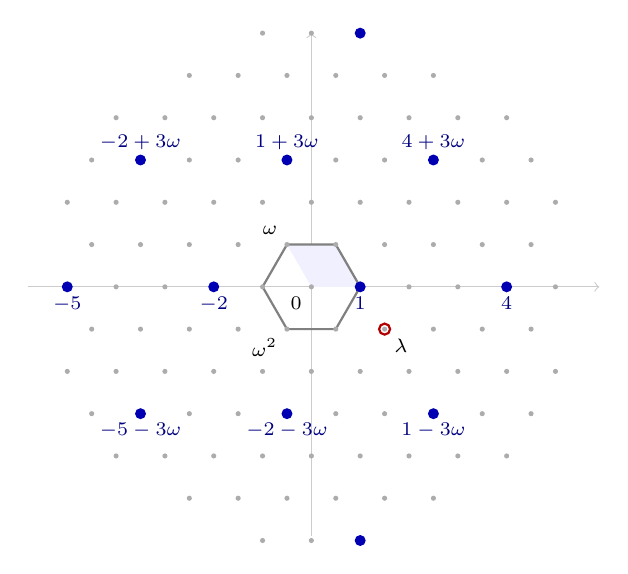
\begin{tikzpicture}[scale=0.62]
\draw[gray!40,->] (-5.8,0)--(5.9,0); \draw[gray!40,->] (0,-5.1)--(0,5.2);
\fill[blue!6] (0,0)--(1,0)--(0.5,0.8660)--(-0.5,0.8660)--cycle;
\draw[thick,gray] (1.0000,0.0000)--(0.5000,0.8660)--(-0.5000,0.8660)--(-1.0000,0.0000)--(-0.5000,-0.8660)--(0.5000,-0.8660)--(1.0000,0.0000);
\fill[gray!65] (-4.0000,-3.4641) circle (1.5pt);
\fill[gray!65] (-4.5000,-2.5981) circle (1.5pt);
\fill[gray!65] (-5.0000,-1.7321) circle (1.5pt);
\fill[gray!65] (-2.5000,-4.3301) circle (1.5pt);
\fill[gray!65] (-3.0000,-3.4641) circle (1.5pt);
\fill[blue!70!black] (-3.5000,-2.5981) circle (3.2pt);
\fill[gray!65] (-4.0000,-1.7321) circle (1.5pt);
\fill[gray!65] (-4.5000,-0.8660) circle (1.5pt);
\fill[blue!70!black] (-5.0000,0.0000) circle (3.2pt);
\fill[gray!65] (-1.0000,-5.1962) circle (1.5pt);
\fill[gray!65] (-1.5000,-4.3301) circle (1.5pt);
\fill[gray!65] (-2.0000,-3.4641) circle (1.5pt);
\fill[gray!65] (-2.5000,-2.5981) circle (1.5pt);
\fill[gray!65] (-3.0000,-1.7321) circle (1.5pt);
\fill[gray!65] (-3.5000,-0.8660) circle (1.5pt);
\fill[gray!65] (-4.0000,0.0000) circle (1.5pt);
\fill[gray!65] (-4.5000,0.8660) circle (1.5pt);
\fill[gray!65] (-5.0000,1.7321) circle (1.5pt);
\fill[gray!65] (0.0000,-5.1962) circle (1.5pt);
\fill[gray!65] (-0.5000,-4.3301) circle (1.5pt);
\fill[gray!65] (-1.0000,-3.4641) circle (1.5pt);
\fill[gray!65] (-1.5000,-2.5981) circle (1.5pt);
\fill[gray!65] (-2.0000,-1.7321) circle (1.5pt);
\fill[gray!65] (-2.5000,-0.8660) circle (1.5pt);
\fill[gray!65] (-3.0000,0.0000) circle (1.5pt);
\fill[gray!65] (-3.5000,0.8660) circle (1.5pt);
\fill[gray!65] (-4.0000,1.7321) circle (1.5pt);
\fill[gray!65] (-4.5000,2.5981) circle (1.5pt);
\fill[blue!70!black] (1.0000,-5.1962) circle (3.2pt);
\fill[gray!65] (0.5000,-4.3301) circle (1.5pt);
\fill[gray!65] (0.0000,-3.4641) circle (1.5pt);
\fill[blue!70!black] (-0.5000,-2.5981) circle (3.2pt);
\fill[gray!65] (-1.0000,-1.7321) circle (1.5pt);
\fill[gray!65] (-1.5000,-0.8660) circle (1.5pt);
\fill[blue!70!black] (-2.0000,0.0000) circle (3.2pt);
\fill[gray!65] (-2.5000,0.8660) circle (1.5pt);
\fill[gray!65] (-3.0000,1.7321) circle (1.5pt);
\fill[blue!70!black] (-3.5000,2.5981) circle (3.2pt);
\fill[gray!65] (-4.0000,3.4641) circle (1.5pt);
\fill[gray!65] (1.5000,-4.3301) circle (1.5pt);
\fill[gray!65] (1.0000,-3.4641) circle (1.5pt);
\fill[gray!65] (0.5000,-2.5981) circle (1.5pt);
\fill[gray!65] (0.0000,-1.7321) circle (1.5pt);
\fill[gray!65] (-0.5000,-0.8660) circle (1.5pt);
\fill[gray!65] (-1.0000,0.0000) circle (1.5pt);
\fill[gray!65] (-1.5000,0.8660) circle (1.5pt);
\fill[gray!65] (-2.0000,1.7321) circle (1.5pt);
\fill[gray!65] (-2.5000,2.5981) circle (1.5pt);
\fill[gray!65] (-3.0000,3.4641) circle (1.5pt);
\fill[gray!65] (2.5000,-4.3301) circle (1.5pt);
\fill[gray!65] (2.0000,-3.4641) circle (1.5pt);
\fill[gray!65] (1.5000,-2.5981) circle (1.5pt);
\fill[gray!65] (1.0000,-1.7321) circle (1.5pt);
\fill[gray!65] (0.5000,-0.8660) circle (1.5pt);
\fill[gray!65] (0.0000,0.0000) circle (1.5pt);
\fill[gray!65] (-0.5000,0.8660) circle (1.5pt);
\fill[gray!65] (-1.0000,1.7321) circle (1.5pt);
\fill[gray!65] (-1.5000,2.5981) circle (1.5pt);
\fill[gray!65] (-2.0000,3.4641) circle (1.5pt);
\fill[gray!65] (-2.5000,4.3301) circle (1.5pt);
\fill[gray!65] (3.0000,-3.4641) circle (1.5pt);
\fill[blue!70!black] (2.5000,-2.5981) circle (3.2pt);
\fill[gray!65] (2.0000,-1.7321) circle (1.5pt);
\fill[gray!65] (1.5000,-0.8660) circle (1.5pt);
\fill[blue!70!black] (1.0000,0.0000) circle (3.2pt);
\fill[gray!65] (0.5000,0.8660) circle (1.5pt);
\fill[gray!65] (0.0000,1.7321) circle (1.5pt);
\fill[blue!70!black] (-0.5000,2.5981) circle (3.2pt);
\fill[gray!65] (-1.0000,3.4641) circle (1.5pt);
\fill[gray!65] (-1.5000,4.3301) circle (1.5pt);
\fill[gray!65] (4.0000,-3.4641) circle (1.5pt);
\fill[gray!65] (3.5000,-2.5981) circle (1.5pt);
\fill[gray!65] (3.0000,-1.7321) circle (1.5pt);
\fill[gray!65] (2.5000,-0.8660) circle (1.5pt);
\fill[gray!65] (2.0000,0.0000) circle (1.5pt);
\fill[gray!65] (1.5000,0.8660) circle (1.5pt);
\fill[gray!65] (1.0000,1.7321) circle (1.5pt);
\fill[gray!65] (0.5000,2.5981) circle (1.5pt);
\fill[gray!65] (0.0000,3.4641) circle (1.5pt);
\fill[gray!65] (-0.5000,4.3301) circle (1.5pt);
\fill[gray!65] (-1.0000,5.1962) circle (1.5pt);
\fill[gray!65] (4.5000,-2.5981) circle (1.5pt);
\fill[gray!65] (4.0000,-1.7321) circle (1.5pt);
\fill[gray!65] (3.5000,-0.8660) circle (1.5pt);
\fill[gray!65] (3.0000,0.0000) circle (1.5pt);
\fill[gray!65] (2.5000,0.8660) circle (1.5pt);
\fill[gray!65] (2.0000,1.7321) circle (1.5pt);
\fill[gray!65] (1.5000,2.5981) circle (1.5pt);
\fill[gray!65] (1.0000,3.4641) circle (1.5pt);
\fill[gray!65] (0.5000,4.3301) circle (1.5pt);
\fill[gray!65] (0.0000,5.1962) circle (1.5pt);
\fill[gray!65] (5.0000,-1.7321) circle (1.5pt);
\fill[gray!65] (4.5000,-0.8660) circle (1.5pt);
\fill[blue!70!black] (4.0000,0.0000) circle (3.2pt);
\fill[gray!65] (3.5000,0.8660) circle (1.5pt);
\fill[gray!65] (3.0000,1.7321) circle (1.5pt);
\fill[blue!70!black] (2.5000,2.5981) circle (3.2pt);
\fill[gray!65] (2.0000,3.4641) circle (1.5pt);
\fill[gray!65] (1.5000,4.3301) circle (1.5pt);
\fill[blue!70!black] (1.0000,5.1962) circle (3.2pt);
\fill[gray!65] (5.0000,0.0000) circle (1.5pt);
\fill[gray!65] (4.5000,0.8660) circle (1.5pt);
\fill[gray!65] (4.0000,1.7321) circle (1.5pt);
\fill[gray!65] (3.5000,2.5981) circle (1.5pt);
\fill[gray!65] (3.0000,3.4641) circle (1.5pt);
\fill[gray!65] (2.5000,4.3301) circle (1.5pt);
\fill[gray!65] (5.0000,1.7321) circle (1.5pt);
\fill[gray!65] (4.5000,2.5981) circle (1.5pt);
\fill[gray!65] (4.0000,3.4641) circle (1.5pt);
\node[below,font=\scriptsize,blue!50!black] at (1.0000,0.0000) {$1$};
\node[below,font=\scriptsize,blue!50!black] at (-2.0000,0.0000) {$-2$};
\node[above,font=\scriptsize,blue!50!black] at (-0.5000,2.5981) {$1+3\omega$};
\node[below,font=\scriptsize,blue!50!black] at (-0.5000,-2.5981) {$-2-3\omega$};
\node[above,font=\scriptsize,blue!50!black] at (2.5000,2.5981) {$4+3\omega$};
\node[below,font=\scriptsize,blue!50!black] at (2.5000,-2.5981) {$1-3\omega$};
\node[above,font=\scriptsize,blue!50!black] at (-3.5000,2.5981) {$-2+3\omega$};
\node[below,font=\scriptsize,blue!50!black] at (-3.5000,-2.5981) {$-5-3\omega$};
\node[below,font=\scriptsize,blue!50!black] at (4.0000,0.0000) {$4$};
\node[below,font=\scriptsize,blue!50!black] at (-5.0000,0.0000) {$-5$};
\node[above left,font=\scriptsize] at (-0.5000,0.8660) {$\omega$};
\node[below left,font=\scriptsize] at (-0.5000,-0.8660) {$\omega^2$};
\node[below right,font=\scriptsize] at (1.5000,-0.8660) {$\lambda$};
\node[below left,font=\scriptsize] at (0.0000,0.0000) {$0$};
\draw[red!70!black,thick] (1.5000,-0.8660) circle (3.2pt);
\end{tikzpicture}

\caption{The Eisenstein integers $a+b\omega$, plotted at $(a-\frac b2,\frac{\sqrt3}2b)$.
The six units form the grey hexagon, the shaded parallelogram is a fundamental domain, and
$\lambda=1-\omega$ is circled. The large dots are the \emph{primary} elements, those
$\equiv1\pmod 3$. They form the translated sublattice $1+3\OO$ (one point in nine), and
each nonzero ideal prime to $3$ has exactly one of them as a generator.}
\label{fig:lattice}
\end{figure}

\subsection{Units}
\begin{proposition}
$\OO^\times=\{\pm1,\pm\omega,\pm\omega^2\}=\langle\zeta\rangle$, where $\zeta=1+\omega=-\omega^2=e^{\pi i/3}$.
This is cyclic of order $6$.
\end{proposition}
\begin{proof}
$\N(a+b\omega)=1$ means $(2a-b)^2+3b^2=4$, so $|b|\le1$. If $b=0$ then $a=\pm1$; if $b=1$ then
$a\in\{0,1\}$, giving $\omega,1+\omega$; if $b=-1$ then $a\in\{0,-1\}$, giving $-\omega,-1-\omega$.
\end{proof}

\subsection{Division with remainder}
\begin{proposition}\label{prop:euclid}
For $\alpha,\beta\in\OO$ with $\beta\ne0$ there are $q,r\in\OO$ with $\alpha=q\beta+r$ and
$\N r\le\frac34\N\beta$. Hence $\OO$ is Euclidean, so it is a PID and a UFD, and $h=1$.
\end{proposition}
\begin{proof}
Write $\alpha/\beta=s+t\omega$ with $s,t\in\Q$, and choose $m,n\in\Z$ with $|s-m|,|t-n|\le\frac12$.
Put $q=m+n\omega$. With $u=s-m$ and $v=t-n$,
$\N(\alpha/\beta-q)=u^2-uv+v^2\le u^2+|u||v|+v^2\le\frac34$. So $r=\alpha-q\beta$ has
$\N r\le\frac34\N\beta$.
\end{proof}
(The hexagonal geometry gives the sharp constant $\frac13$: every point of $\mathbb C$ lies
within $1/\sqrt3$ of the lattice.)

\begin{example}[Finding a prime of norm $61$]\label{ex:euclid}
Since $13^2+13+1=183=3\cdot61$, $r=13$ is a root of $x^2+x+1$ modulo $61$, and
$\gcd(61,13-\omega)$ is a prime above $61$. We have
$\frac{61}{13-\omega}=\frac{61(13-\bar\omega)}{183}=\frac{14+\omega}3$, which rounds to $q=5$.
The Euclidean algorithm runs
\begin{equation}\label{eq:euclid61}
 61=5\,(13-\omega)+(-4+5\omega),\qquad
 13-\omega=(-2-\omega)(-4+5\omega)+0 .
\end{equation}
So $\gcd(61,13-\omega)=-4+5\omega$, of norm $16+20+25=61$. Its primary associate
(\S\ref{sec:primary}) is $\omega(-4+5\omega)=-5-9\omega$, and
$61=(-5-9\omega)(4+9\omega)$. (The cofactor $-2-\omega=\omega^2\lambda$ has norm $3$.)
\end{example}

\subsection{The prime \texorpdfstring{$\lambda$}{lambda} and residues modulo \texorpdfstring{$3$}{3}}
Put $\lambda=1-\omega$, so $\N\lambda=3$. Then
\begin{equation}\label{eq:lambda}
 \lambda^2=-3\omega,\qquad 3=-\omega^2\lambda^2,\qquad \bar\lambda=1-\omega^2=-\omega^2\lambda,
 \qquad \sqrt{-3}=\omega\lambda,
\end{equation}
so $(3)=(\lambda)^2$: the prime $3$ ramifies. Since $\omega\equiv1\pmod\lambda$, we have
$a+b\omega\equiv a+b\pmod\lambda$. Hence
\begin{equation}\label{eq:modlambda}
 \OO/\lambda\cong\F_3=\{0,1,-1\},\qquad \lambda\mid a+b\omega\iff 3\mid a+b .
\end{equation}
The ring $\OO/3=\OO/\lambda^2$ has $9$ elements $a+b\omega$ ($a,b$ modulo $3$). Its unit
group has $6$ elements, represented exactly by the six units (see
Proposition~\ref{prop:primary}). Also $\N(a+b\omega)=(a+b)^2-3ab\equiv(a+b)^2\pmod 3$, so
every $\alpha$ prime to $3$ has $\N\alpha\equiv1\pmod 3$. For later use,
$\OO/2\cong\F_4=\{0,1,\omega,\omega^2\}$.

\subsection{Primes of \texorpdfstring{$\OO$}{Z[omega]} and the factorization of rational primes}\label{sec:primes}
\begin{theorem}\label{thm:primes}
Up to units, the primes of $\OO$ are the following.
\begin{enumerate}
\item $\lambda=1-\omega$, with $\N\lambda=3$ and $3=-\omega^2\lambda^2$ \emph{(3 ramifies)}.
\item For each prime $p\equiv1\pmod3$, two conjugate primes $\pi,\bar\pi$ that are not
associates, with $p=\pi\bar\pi$ and $\N\pi=\N\bar\pi=p$ \emph{($p$ splits)}.
\item For each prime $p\equiv2\pmod3$, the prime $p$ itself, with $\N p=p^2$ \emph{($p$ is inert)}.
\end{enumerate}
So $p$ splits, is inert, or ramifies according as $\ch(p)=\bigl(\frac p3\bigr)$ is $1$, $-1$
or $0$. This agrees with Theorem~\ref{thm:splitting}, since $\bigl(\frac{-3}p\bigr)=\bigl(\frac p3\bigr)$
by quadratic reciprocity.
\end{theorem}

\begin{proof}
Let $\pi$ be a prime of $\OO$. Since $\pi\mid\pi\bar\pi=\N\pi\in\Z$, $\pi$ divides a
rational prime $p$, and only one: if $\pi\mid p$ and $\pi\mid q\ne p$ then $\pi\mid1$. Then
$\N\pi\mid\N p=p^2$. If $\N\pi=p^2$, then $p/\pi$ is a unit and $\pi\sim p$. If $\N\pi=p$, then
$p=\pi\bar\pi$. It remains to decide, for each $p$, whether an element of norm $p$ exists.
(An element of prime norm is irreducible, hence prime, since $\OO$ is a UFD.)

\emph{$p=3$:} $\lambda$ has norm $3$.

\emph{$p\equiv2\pmod3$:} $4\N(a+b\omega)=(2a-b)^2+3b^2\equiv(2a-b)^2\pmod3$, while
$4p\equiv2\pmod 3$ is not a square modulo $3$. So no element has norm $p$, and $p$ is prime in $\OO$.

\emph{$p\equiv1\pmod3$:} $\F_p^\times$ is cyclic of order divisible by $3$, so some $r\in\Z$
has $r^2+r+1\equiv0\pmod p$. Then $p\mid(r-\omega)(r-\bar\omega)=r^2+r+1$, but $p$ divides
neither factor (their $\omega$-coordinates are $\mp1$). So $p$ is not prime, and $p=\pi\bar\pi$ with
$\N\pi=p$. The prime $\pi$ divides one factor, say $r-\omega$, and then $\bar\pi\mid r-\bar\omega$.
If $\bar\pi$ were an associate of $\pi$, then $\pi$ would divide both factors and hence
their difference $\omega-\bar\omega=\sqrt{-3}$, so $p\mid\N\sqrt{-3}=3$, which is false.
\end{proof}

\begin{corollary}[Fermat, Euler, Gauss]\label{cor:forms}
Let $p\ne3$ be prime.
\begin{enumerate}
\item $p=a^2-ab+b^2$ for some $a,b\in\Z$ $\iff$ $p=x^2+3y^2$ for some $x,y\in\Z$ $\iff$ $p\equiv1\pmod 3$.
\item If $p\equiv1\pmod3$, then $4p=L^2+27M^2$ with $L\equiv1\pmod 3$, and $L$ is
unique while $M$ is unique up to sign. If $\pi=a+b\omega$ is either primary prime above $p$
(\S\ref{sec:primary}), then $L=-\Tr\pi=b-2a$ and $M=\pm b/3$.
\end{enumerate}
\end{corollary}
\begin{proof}
(1) An element of norm $p$ exists iff $p\equiv1\pmod 3$. Among $\alpha,\omega\alpha,\omega^2\alpha$
the $\omega$-coordinates are $b$, $a-b$ and $-a$. Since $p$ is odd, $a$ and $b$ are not both
even, and then one of these three is even. Using that associate,
$p=(a-\frac b2)^2+3(\frac b2)^2$. (2) For primary $\pi=a+b\omega$ we have $3\mid b$, and
$4p=(2a-b)^2+3b^2$. Conversely, if $4p=L^2+27M^2$, then $L\equiv M\pmod2$, and
$\frac{L+3M\sqrt{-3}}2=\frac{L+3M}2+3M\omega$ is an element of norm $p$ whose
$\omega$-coordinate is divisible by $3$. It is therefore $\pm$ a primary prime above $p$, and
$L$ is determined up to sign. Since $a\equiv1$ and $b\equiv0\pmod 3$, $-\Tr\pi=b-2a\equiv1\pmod 3$,
which fixes the sign.
\end{proof}

\paragraph{Residue fields.} If $p\equiv1\pmod3$ and $\pi=a+b\omega$ has norm $p$, then
$\OO/\pi\cong\F_p$, and the isomorphism sends $\omega\mapsto r\equiv-a\,b^{-1}\pmod p$. (Here $p\nmid b$:
otherwise $p\mid a$, and then $p^2\mid\N\pi$.) The value $r$ is a root of $x^2+x+1$, and $\bar\pi$
corresponds to the other root $r^2$. If $p\equiv2\pmod3$, then $\OO/p\cong\F_{p^2}$.

\paragraph{Galois view.} $K=\Q(\zeta_3)$, and for $p\ne3$ the Frobenius at $p$ is
$\zeta_3\mapsto\zeta_3^p$. It is trivial exactly when $p\equiv1\pmod3$, the case in which $p$ splits.

\subsection{Primary elements}\label{sec:primary}
\begin{definition}
$\alpha\in\OO$ is \emph{primary} if $\alpha\equiv1\pmod 3$. In coordinates,
$a+b\omega$ is primary $\iff a\equiv1$ and $b\equiv0\pmod 3$.
\end{definition}

\begin{remark}[Conventions]
This is the convention of the OpenAI quasi-Riemann hypothesis papers \cite{OAI} (and of our
guides to them). Ireland and Rosen \cite[Ch.~9]{IR} instead call a prime primary if it is
$\equiv2\pmod3$, which is $-1$ times ours. Some authors use $\equiv\pm1\pmod 3$
(``semi-primary''; each ideal prime to $3$ has two such generators). Cubic residue symbols
do not see the difference, since $-1=(-1)^3$ is a cube. The Gauss and Jacobi sums of
\S\ref{sec:gauss}, and the integer $L\equiv1\pmod3$ in $4p=L^2+27M^2$, are unchanged.
Their expressions in terms of the chosen generator have different signs: with $\pi'=-\pi$,
$J=-\pi=\pi'$, $g^3=-p\pi=p\pi'$, and $L=-\Tr\pi=\Tr\pi'$.
\end{remark}

\begin{proposition}\label{prop:primary}
\begin{enumerate}
\item Every $\alpha$ prime to $3$ has exactly one primary associate. Hence every nonzero
ideal prime to $3$ has exactly one primary generator.
\item Products and conjugates of primary elements are primary. A rational integer $n$ is
primary iff $n\equiv1\pmod 3$; for instance $-2,4,-5,7,\dots$. In particular, for
$p\equiv2\pmod 3$ the primary generator of $(p)$ is $-p$.
\item Every primary element is uniquely a product of primary primes, \emph{with no unit
factor}. In particular, if $p\equiv1\pmod3$, then $p=\pi\bar\pi$ exactly, with $\pi,\bar\pi$ primary.
\end{enumerate}
\end{proposition}
\begin{proof}
(1) Distinct units are incongruent modulo $3$: if $u\ne u'$, then $0<\N(u-u')\le4<9=\N3$. So the
six units represent the six classes of $(\OO/3)^\times$. If $\alpha$ is prime to $3$, it is
invertible modulo $3$, and exactly one unit $u$ satisfies $u\equiv\alpha^{-1}$, i.e.\
$u\alpha\equiv1\pmod 3$. (2) $\bar 3=3$ and $\bar1=1$. (3) Write $\alpha=u\prod\pi_i$ with primary primes
$\pi_i$, using unique factorization and (1); no $\pi_i$ is $\lambda$ because $\alpha$ is prime to $3$.
The product $\prod\pi_i$ is primary, so $u\equiv1\pmod 3$, and $u=1$ by (1). For the last claim
note that $p\equiv1\pmod 3$ is itself primary.
\end{proof}

So primary elements correspond one-to-one to the nonzero ideals prime to $3$, and
\begin{equation}\label{eq:primaryzeta}
 \sum_{\alpha\ \mathrm{primary}}\N\alpha^{-s}=(1-3^{-s})\,\zeta_K(s).
\end{equation}
The primary primes of norm below $50$ are
\begin{equation}\label{eq:smallprimes}
\begin{gathered}
 -2\ (4),\quad 1+3\omega,\ -2-3\omega\ (7),\quad 4+3\omega,\ 1-3\omega\ (13),\quad
 -2+3\omega,\ -5-3\omega\ (19),\quad -5\ (25),\\
 1+6\omega,\ -5-6\omega\ (31),\quad 7+3\omega,\ 4-3\omega\ (37),\quad 7+6\omega,\ 1-6\omega\ (43),
\end{gathered}
\end{equation}
with norms in parentheses. Table~\ref{tab:primary} lists all primary elements of norm at most $100$.

\subsection{Ideals of \texorpdfstring{$\OO$}{Z[omega]} as lattices}\label{sec:ideals}
Since $\OO=\Z+\Z\omega$, an additive subgroup $I\subseteq\OO$ is an ideal as soon as $\omega I\subseteq I$.
Multiplication by $\omega$ is the rotation through $120^\circ$, and $I=-I$. So \emph{the nonzero ideals of
$\OO$ are the nonzero subgroups of $\OO$ that are mapped to themselves by the rotation through $60^\circ$},
which is multiplication by the unit $1+\omega=e^{\pi i/3}$. Such a subgroup contains $\N\alpha$ and
$\N\alpha\,\omega$ for each of its elements $\alpha\ne0$, so it is a sublattice of finite index.

Every ideal is principal (Proposition~\ref{prop:euclid}):
\begin{equation}\label{eq:principal}
 I=(\alpha)=\alpha\OO=\Z\alpha+\Z\,\omega\alpha .
\end{equation}
As a map of $\mathbb C$, multiplication by $\alpha$ is the rotation through $\arg\alpha$ followed by the
dilation by $|\alpha|=\sqrt{\N\alpha}$. So $(\alpha)$ is a rotated and enlarged copy of the hexagonal
lattice $\OO$. This has three consequences.
\begin{itemize}
\item \emph{Generators.} The generators of $(\alpha)$ are its six elements $u\alpha$, $u$ a unit. They are
the nonzero elements of $(\alpha)$ nearest to $0$, and they are the vertices of a regular hexagon of radius
$\sqrt{\N\alpha}$, just as the units are for $\OO$. If $(\alpha)$ is prime to $3$, exactly one of them is
primary (Proposition~\ref{prop:primary}).
\item \emph{Norm, index and area.} The parallelogram spanned by $\alpha$ and $\omega\alpha$ is a fundamental
domain of $(\alpha)$. Its area is $\N\alpha\cdot\frac{\sqrt3}2$, which is $\N\alpha$ times the area of a
fundamental domain of $\OO$. The index of a sublattice is the ratio of these areas, so
\begin{equation}\label{eq:index}
 \N\alpha=[\OO:(\alpha)]=|\OO/(\alpha)| .
\end{equation}
The points of $\OO$ in the half-open parallelogram $\{s\alpha+t\omega\alpha:0\le s,t<1\}$ form a complete
set of residues modulo $\alpha$.
\item \emph{Operations.} For ideals $I=(\alpha)$ and $J=(\beta)$,
\begin{equation}\label{eq:idealops}
 I+J=(\gcd(\alpha,\beta)),\qquad I\cap J=(\operatorname{lcm}(\alpha,\beta)),\qquad IJ=(\alpha\beta),\qquad
 \N(IJ)=\N I\cdot\N J .
\end{equation}
Here $IJ$ is the set of finite sums of products $xy$ with $x\in I$ and $y\in J$; if $I=(\alpha_1,\alpha_2)$ and
$J=(\beta_1,\beta_2)$, it is generated by the four products $\alpha_i\beta_j$. Also $I\supseteq J$ if and only
if $I\mid J$: \emph{to contain is to divide}. If $I+J=\OO$, i.e.\ $I$ and $J$ are coprime, then $IJ=I\cap J$,
and the Chinese remainder theorem gives $\OO/IJ\cong\OO/I\times\OO/J$. Without coprimality the product can be
smaller than the intersection; for example $(\lambda)(\lambda)=(3)$ but $(\lambda)\cap(\lambda)=(\lambda)$.
\end{itemize}

The next proposition lists all ideals explicitly in coordinates.

\begin{proposition}[Ideals in coordinates]\label{prop:idealcoords}
\begin{enumerate}
\item Let $m\ge1$, and let $r\in\Z$ satisfy $r^2+r+1\equiv0\pmod m$. Then $x+y\omega\mapsto x+ry\bmod m$ is a
ring homomorphism from $\OO$ onto $\Z/m\Z$, and its kernel
\begin{equation}\label{eq:Imr}
 I_{m,r}=\{x+y\omega:\ x+ry\equiv0\pmod m\}=\Z m+\Z(\omega-r)
\end{equation}
is an ideal of norm $m$. It depends only on $r$ modulo $m$.
\item Every nonzero ideal equals $c\,I_{m,r}$ for exactly one integer $c\ge1$, one $m\ge1$ and one $r$ modulo
$m$ with $r^2+r+1\equiv0\pmod m$. Here $c$ is the gcd of the coordinates of the elements of the ideal, and the
norm of the ideal is $c^2m$.
\item Hence, if $\varrho(m)$ is the number of $r$ modulo $m$ with $r^2+r+1\equiv0\pmod m$, the number of ideals
of norm $n$ is $\sum_{c^2\mid n}\varrho(n/c^2)$.
\end{enumerate}
\end{proposition}

\begin{proof}
(1) The map is additive and sends $1$ to $1$, so it is onto, and its kernel has index $m$. By
\eqref{eq:arith}, $(x+y\omega)(x'+y'\omega)=(xx'-yy')+(xy'+x'y-yy')\,\omega$, and
\begin{equation}\label{eq:homcheck}
 (x+ry)(x'+ry')-\bigl(xx'-yy'+r(xy'+x'y-yy')\bigr)=yy'(r^2+r+1)\equiv0\pmod m,
\end{equation}
so the map is multiplicative and its kernel is an ideal. Both $m$ and $\omega-r$ lie in the kernel. Conversely,
if $x+ry\equiv0\pmod m$, then $x+y\omega=y(\omega-r)+(x+ry)\in\Z(\omega-r)+\Z m$.

(2) Let $I\ne0$, let $c$ be the gcd of the coordinates of its elements, and put $J=c^{-1}I$. This is an
ideal, and the coordinates of its elements have gcd $1$. The $\omega$-coordinates of the elements of $J$
form a subgroup $d\Z$ of $\Z$. If $x+y\omega\in J$, then $\omega(x+y\omega)=-y+(x-y)\omega\in J$, so $d\mid y$
and $d\mid x-y$, hence $d\mid x$. Thus $d$ divides every coordinate, and $d=1$. So $J$ contains an element
$\omega-r$ with $r\in\Z$. Also $J\cap\Z=m\Z$ for some $m\ge1$. If $x+y\omega\in J$, then
$x+ry=(x+y\omega)-y(\omega-r)\in J\cap\Z$, so $J=\Z m+\Z(\omega-r)=I_{m,r}$. Finally
$\omega(\omega-r)=-(1+r)(\omega-r)-(r^2+r+1)$ lies in $J$, so $r^2+r+1\in J\cap\Z=m\Z$. The data are
unique: $c$ is determined by $I$, $m$ by $J\cap\Z=m\Z$, and $r$ modulo $m$ because $\omega-r$ and
$\omega-r'$ in $J$ imply $r'-r\in J\cap\Z$. The norm is $[\OO:c\OO]\,[c\OO:cJ]=c^2m$.

(3) This follows from (2).
\end{proof}

By the Chinese remainder theorem $\varrho$ is multiplicative. Also $\varrho(3)=1$ (the root is $r=1$) and
$\varrho(9)=0$, so $\varrho(3^k)=0$ for $k\ge2$. For a prime $p\ne3$, $x^2+x+1$ has a root modulo $p$ if and only if
$p\equiv1\pmod3$ (proof of Theorem~\ref{thm:primes}), and then it has two. Since $(2r+1)^2=4(r^2+r+1)-3$, the
derivative $2r+1$ of $x^2+x+1$ at a root is prime to $p$, so by Hensel's lemma $\varrho(p^k)=1+\ch(p)$ for all $k\ge1$.
With these values, part (3) agrees with \eqref{eq:countideals}; we also checked this for every $n\le3000$.

\paragraph{Prime ideals in coordinates.} The prime ideals of Theorem~\ref{thm:primes} are as follows.
\begin{itemize}
\item $(\lambda)=I_{3,1}=\{x+y\omega:3\mid x+y\}$, the kernel of the reduction $\OO\to\F_3$, $\omega\mapsto1$
(\S\ref{sec:primes}).
\item If $p\equiv1\pmod3$, let $r$ and $r'=-1-r$ be the two roots of $x^2+x+1$ modulo $p$. The two primes
above $p$ are $\mathfrak p=I_{p,r}$ and $\bar{\mathfrak p}=I_{p,r'}$, the kernels of the two homomorphisms
$\OO\to\F_p$ that send $\omega$ to $r$ and to $r'$. Complex conjugation exchanges them, since
$\overline{x+y\omega}=(x-y)-y\omega$ and $(x-y)+r(-y)=x+r'y$. A generator is $\gcd(p,\omega-r)$, which the
Euclidean algorithm finds; in Example~\ref{ex:euclid}, $I_{61,13}=(-5-9\omega)$.
\item If $p\equiv2\pmod 3$, then $(p)=p\,I_{1,0}=p\OO$, a copy of $\OO$ scaled by $p$.
\end{itemize}
For $p=7$ the roots of $x^2+x+1$ are $2$ and $4$, and
\begin{equation}\label{eq:p7}
 \mathfrak p=I_{7,2}=(7,\omega-2)=(1+3\omega),\qquad \bar{\mathfrak p}=I_{7,4}=(7,\omega-4)=(-2-3\omega),
\end{equation}
since $1+2\cdot3=7$ and $-2+4\cdot(-3)=-14$. The six generators of $\mathfrak p$ are $\pm\pi$, $\pm\omega\pi$ and
$\pm\omega^2\pi$, where $\pi=1+3\omega$, $\omega\pi=-3-2\omega$ and $\omega^2\pi=2-\omega$. In particular
$\omega-2=-\omega^2\pi=(1+\omega)\pi$ is a generator, so $\mathfrak p=(\omega-2)$. Figure~\ref{fig:ideal-p7}
shows $\mathfrak p$, and Figure~\ref{fig:ideal-ram-inert} shows $(\lambda)$ and $(2)$.

\begin{example}[Products]\label{ex:products}
With the two-element generators of \eqref{eq:p7}, $\mathfrak p\bar{\mathfrak p}$ is generated by the four
products of generators:
\begin{equation}\label{eq:ppbar}
 \mathfrak p\bar{\mathfrak p}=\bigl(49,\ 7(\omega-4),\ 7(\omega-2),\ (\omega-2)(\omega-4)\bigr)
 =\bigl(49,\ 7\omega-28,\ 7\omega-14,\ 7-7\omega\bigr)=(7).
\end{equation}
Indeed, every generator is a multiple of $7$, and $7=49-3\bigl((7\omega-14)-(7\omega-28)\bigr)$ lies in the
ideal. As $\mathfrak p$ and $\bar{\mathfrak p}$ are coprime, $\mathfrak p\bar{\mathfrak p}=\mathfrak p\cap
\bar{\mathfrak p}$: the ideal $(7)$ consists of the points common to the two lattices
(Figure~\ref{fig:ideal-products}, left). The Chinese remainder theorem gives
$\OO/(7)\cong\F_7\times\F_7$, $x+y\omega\mapsto(x+2y,\,x+4y)$. In the same way
\begin{equation}\label{eq:psquare}
 \mathfrak p^2=\bigl(49,\ 7(\omega-2),\ (\omega-2)^2\bigr)=(3-5\omega)=(\pi^2)=(-8-3\omega)=I_{49,30},
\end{equation}
because $(\omega-2)^2=3-5\omega=\omega\pi^2$ already generates $\mathfrak p^2$. Here $30$ is the root of
$r^2+r+1\equiv0\pmod{49}$ with $r\equiv2\pmod7$, and $-8+30\cdot(-3)=-98$. The ideal $\mathfrak p^2$ has
index $7$ in $\mathfrak p$ (Figure~\ref{fig:ideal-products}, right). So $\mathfrak p\cdot\mathfrak p$ is strictly smaller
than $\mathfrak p\cap\mathfrak p=\mathfrak p$, unlike the coprime product $\mathfrak p\bar{\mathfrak p}=\mathfrak p\cap\bar{\mathfrak p}$.
The three ideals
of norm $49$ are $\mathfrak p^2=I_{49,30}$, $\bar{\mathfrak p}^2=I_{49,18}$ and $\mathfrak p\bar{\mathfrak p}=7I_{1,0}$,
in agreement with $\varrho(49)+\varrho(1)=3=\sum_{d\mid49}\ch(d)$. Likewise $(\lambda)\mathfrak p=(\lambda)\cap
\mathfrak p=(\lambda\pi)$ has norm $21$, and $(\lambda)^2=(3)$ has index $3$ in $(\lambda)$
(Figure~\ref{fig:ideal-ram-inert}).
\end{example}

\begin{figure}[ht]
\centering
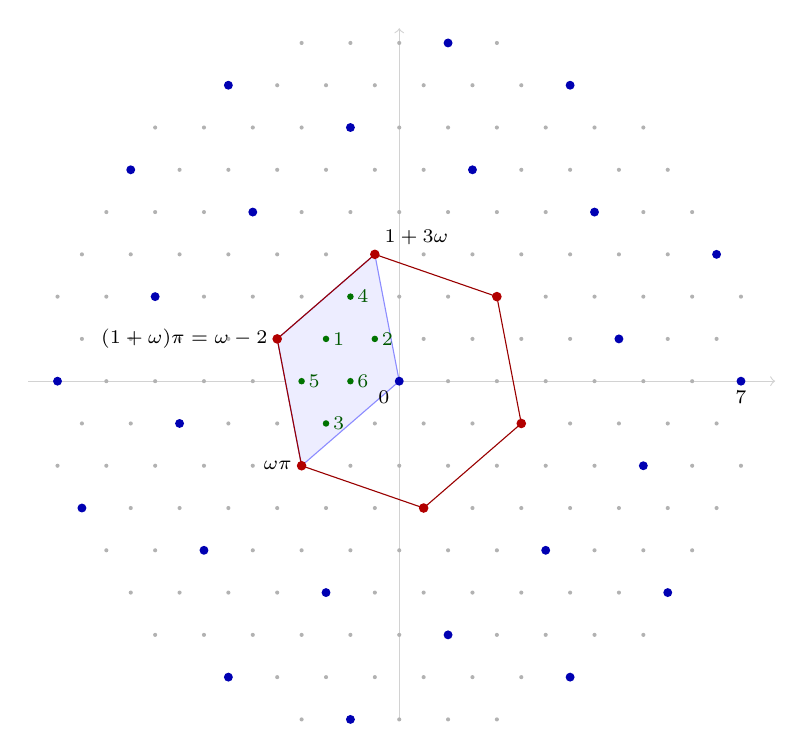
\begin{tikzpicture}[scale=0.62]
\draw[gray!35,->] (-7.60,0)--(7.70,0); \draw[gray!35,->] (0,-6.93)--(0,7.23);
\fill[blue!7] (0.0000,0.0000)--(-0.5000,2.5981)--(-2.5000,0.8660)--(-2.0000,-1.7321)--cycle;
\draw[blue!45] (0.0000,0.0000)--(-0.5000,2.5981)--(-2.5000,0.8660)--(-2.0000,-1.7321)--cycle;
\draw[red!60!black,thin] (-2.0000,-1.7321)--(0.5000,-2.5981)--(2.5000,-0.8660)--(2.0000,1.7321)--(-0.5000,2.5981)--(-2.5000,0.8660)--cycle;
\fill[gray!60] (-5.0000,-5.1962) circle (1.2pt);
\fill[gray!60] (-5.5000,-4.3301) circle (1.2pt);
\fill[gray!60] (-6.0000,-3.4641) circle (1.2pt);
\fill[gray!60] (-7.0000,-1.7321) circle (1.2pt);
\fill[gray!60] (-4.0000,-5.1962) circle (1.2pt);
\fill[gray!60] (-4.5000,-4.3301) circle (1.2pt);
\fill[gray!60] (-5.0000,-3.4641) circle (1.2pt);
\fill[gray!60] (-5.5000,-2.5981) circle (1.2pt);
\fill[gray!60] (-6.0000,-1.7321) circle (1.2pt);
\fill[gray!60] (-6.5000,-0.8660) circle (1.2pt);
\fill[gray!60] (-2.0000,-6.9282) circle (1.2pt);
\fill[gray!60] (-2.5000,-6.0622) circle (1.2pt);
\fill[gray!60] (-3.0000,-5.1962) circle (1.2pt);
\fill[gray!60] (-3.5000,-4.3301) circle (1.2pt);
\fill[gray!60] (-4.5000,-2.5981) circle (1.2pt);
\fill[gray!60] (-5.0000,-1.7321) circle (1.2pt);
\fill[gray!60] (-5.5000,-0.8660) circle (1.2pt);
\fill[gray!60] (-6.0000,0.0000) circle (1.2pt);
\fill[gray!60] (-6.5000,0.8660) circle (1.2pt);
\fill[gray!60] (-7.0000,1.7321) circle (1.2pt);
\fill[gray!60] (-1.5000,-6.0622) circle (1.2pt);
\fill[gray!60] (-2.0000,-5.1962) circle (1.2pt);
\fill[gray!60] (-2.5000,-4.3301) circle (1.2pt);
\fill[gray!60] (-3.0000,-3.4641) circle (1.2pt);
\fill[gray!60] (-3.5000,-2.5981) circle (1.2pt);
\fill[gray!60] (-4.0000,-1.7321) circle (1.2pt);
\fill[gray!60] (-5.0000,0.0000) circle (1.2pt);
\fill[gray!60] (-5.5000,0.8660) circle (1.2pt);
\fill[gray!60] (-6.0000,1.7321) circle (1.2pt);
\fill[gray!60] (-6.5000,2.5981) circle (1.2pt);
\fill[gray!60] (0.0000,-6.9282) circle (1.2pt);
\fill[gray!60] (-0.5000,-6.0622) circle (1.2pt);
\fill[gray!60] (-1.0000,-5.1962) circle (1.2pt);
\fill[gray!60] (-2.0000,-3.4641) circle (1.2pt);
\fill[gray!60] (-2.5000,-2.5981) circle (1.2pt);
\fill[gray!60] (-3.0000,-1.7321) circle (1.2pt);
\fill[gray!60] (-3.5000,-0.8660) circle (1.2pt);
\fill[gray!60] (-4.0000,0.0000) circle (1.2pt);
\fill[gray!60] (-4.5000,0.8660) circle (1.2pt);
\fill[gray!60] (-5.5000,2.5981) circle (1.2pt);
\fill[gray!60] (-6.0000,3.4641) circle (1.2pt);
\fill[gray!60] (1.0000,-6.9282) circle (1.2pt);
\fill[gray!60] (0.5000,-6.0622) circle (1.2pt);
\fill[gray!60] (0.0000,-5.1962) circle (1.2pt);
\fill[gray!60] (-0.5000,-4.3301) circle (1.2pt);
\fill[gray!60] (-1.0000,-3.4641) circle (1.2pt);
\fill[gray!60] (-1.5000,-2.5981) circle (1.2pt);
\fill[gray!60] (-2.5000,-0.8660) circle (1.2pt);
\fill[gray!60] (-3.0000,0.0000) circle (1.2pt);
\fill[gray!60] (-3.5000,0.8660) circle (1.2pt);
\fill[gray!60] (-4.0000,1.7321) circle (1.2pt);
\fill[gray!60] (-4.5000,2.5981) circle (1.2pt);
\fill[gray!60] (-5.0000,3.4641) circle (1.2pt);
\fill[gray!60] (2.0000,-6.9282) circle (1.2pt);
\fill[gray!60] (1.5000,-6.0622) circle (1.2pt);
\fill[gray!60] (0.5000,-4.3301) circle (1.2pt);
\fill[gray!60] (0.0000,-3.4641) circle (1.2pt);
\fill[gray!60] (-0.5000,-2.5981) circle (1.2pt);
\fill[gray!60] (-1.0000,-1.7321) circle (1.2pt);
\fill[gray!60] (-1.5000,-0.8660) circle (1.2pt);
\fill[gray!60] (-2.0000,0.0000) circle (1.2pt);
\fill[gray!60] (-3.0000,1.7321) circle (1.2pt);
\fill[gray!60] (-3.5000,2.5981) circle (1.2pt);
\fill[gray!60] (-4.0000,3.4641) circle (1.2pt);
\fill[gray!60] (-4.5000,4.3301) circle (1.2pt);
\fill[gray!60] (-5.0000,5.1962) circle (1.2pt);
\fill[gray!60] (2.5000,-6.0622) circle (1.2pt);
\fill[gray!60] (2.0000,-5.1962) circle (1.2pt);
\fill[gray!60] (1.5000,-4.3301) circle (1.2pt);
\fill[gray!60] (1.0000,-3.4641) circle (1.2pt);
\fill[gray!60] (0.0000,-1.7321) circle (1.2pt);
\fill[gray!60] (-0.5000,-0.8660) circle (1.2pt);
\fill[gray!60] (-1.0000,0.0000) circle (1.2pt);
\fill[gray!60] (-1.5000,0.8660) circle (1.2pt);
\fill[gray!60] (-2.0000,1.7321) circle (1.2pt);
\fill[gray!60] (-2.5000,2.5981) circle (1.2pt);
\fill[gray!60] (-3.5000,4.3301) circle (1.2pt);
\fill[gray!60] (-4.0000,5.1962) circle (1.2pt);
\fill[gray!60] (3.0000,-5.1962) circle (1.2pt);
\fill[gray!60] (2.5000,-4.3301) circle (1.2pt);
\fill[gray!60] (2.0000,-3.4641) circle (1.2pt);
\fill[gray!60] (1.5000,-2.5981) circle (1.2pt);
\fill[gray!60] (1.0000,-1.7321) circle (1.2pt);
\fill[gray!60] (0.5000,-0.8660) circle (1.2pt);
\fill[gray!60] (-0.5000,0.8660) circle (1.2pt);
\fill[gray!60] (-1.0000,1.7321) circle (1.2pt);
\fill[gray!60] (-1.5000,2.5981) circle (1.2pt);
\fill[gray!60] (-2.0000,3.4641) circle (1.2pt);
\fill[gray!60] (-2.5000,4.3301) circle (1.2pt);
\fill[gray!60] (-3.0000,5.1962) circle (1.2pt);
\fill[gray!60] (4.0000,-5.1962) circle (1.2pt);
\fill[gray!60] (3.5000,-4.3301) circle (1.2pt);
\fill[gray!60] (2.5000,-2.5981) circle (1.2pt);
\fill[gray!60] (2.0000,-1.7321) circle (1.2pt);
\fill[gray!60] (1.5000,-0.8660) circle (1.2pt);
\fill[gray!60] (1.0000,0.0000) circle (1.2pt);
\fill[gray!60] (0.5000,0.8660) circle (1.2pt);
\fill[gray!60] (0.0000,1.7321) circle (1.2pt);
\fill[gray!60] (-1.0000,3.4641) circle (1.2pt);
\fill[gray!60] (-1.5000,4.3301) circle (1.2pt);
\fill[gray!60] (-2.0000,5.1962) circle (1.2pt);
\fill[gray!60] (-2.5000,6.0622) circle (1.2pt);
\fill[gray!60] (5.0000,-5.1962) circle (1.2pt);
\fill[gray!60] (4.5000,-4.3301) circle (1.2pt);
\fill[gray!60] (4.0000,-3.4641) circle (1.2pt);
\fill[gray!60] (3.5000,-2.5981) circle (1.2pt);
\fill[gray!60] (3.0000,-1.7321) circle (1.2pt);
\fill[gray!60] (2.0000,0.0000) circle (1.2pt);
\fill[gray!60] (1.5000,0.8660) circle (1.2pt);
\fill[gray!60] (1.0000,1.7321) circle (1.2pt);
\fill[gray!60] (0.5000,2.5981) circle (1.2pt);
\fill[gray!60] (0.0000,3.4641) circle (1.2pt);
\fill[gray!60] (-0.5000,4.3301) circle (1.2pt);
\fill[gray!60] (-1.5000,6.0622) circle (1.2pt);
\fill[gray!60] (-2.0000,6.9282) circle (1.2pt);
\fill[gray!60] (5.0000,-3.4641) circle (1.2pt);
\fill[gray!60] (4.5000,-2.5981) circle (1.2pt);
\fill[gray!60] (4.0000,-1.7321) circle (1.2pt);
\fill[gray!60] (3.5000,-0.8660) circle (1.2pt);
\fill[gray!60] (3.0000,0.0000) circle (1.2pt);
\fill[gray!60] (2.5000,0.8660) circle (1.2pt);
\fill[gray!60] (1.5000,2.5981) circle (1.2pt);
\fill[gray!60] (1.0000,3.4641) circle (1.2pt);
\fill[gray!60] (0.5000,4.3301) circle (1.2pt);
\fill[gray!60] (0.0000,5.1962) circle (1.2pt);
\fill[gray!60] (-0.5000,6.0622) circle (1.2pt);
\fill[gray!60] (-1.0000,6.9282) circle (1.2pt);
\fill[gray!60] (6.0000,-3.4641) circle (1.2pt);
\fill[gray!60] (5.5000,-2.5981) circle (1.2pt);
\fill[gray!60] (4.5000,-0.8660) circle (1.2pt);
\fill[gray!60] (4.0000,0.0000) circle (1.2pt);
\fill[gray!60] (3.5000,0.8660) circle (1.2pt);
\fill[gray!60] (3.0000,1.7321) circle (1.2pt);
\fill[gray!60] (2.5000,2.5981) circle (1.2pt);
\fill[gray!60] (2.0000,3.4641) circle (1.2pt);
\fill[gray!60] (1.0000,5.1962) circle (1.2pt);
\fill[gray!60] (0.5000,6.0622) circle (1.2pt);
\fill[gray!60] (0.0000,6.9282) circle (1.2pt);
\fill[gray!60] (6.5000,-2.5981) circle (1.2pt);
\fill[gray!60] (6.0000,-1.7321) circle (1.2pt);
\fill[gray!60] (5.5000,-0.8660) circle (1.2pt);
\fill[gray!60] (5.0000,0.0000) circle (1.2pt);
\fill[gray!60] (4.0000,1.7321) circle (1.2pt);
\fill[gray!60] (3.5000,2.5981) circle (1.2pt);
\fill[gray!60] (3.0000,3.4641) circle (1.2pt);
\fill[gray!60] (2.5000,4.3301) circle (1.2pt);
\fill[gray!60] (2.0000,5.1962) circle (1.2pt);
\fill[gray!60] (1.5000,6.0622) circle (1.2pt);
\fill[gray!60] (7.0000,-1.7321) circle (1.2pt);
\fill[gray!60] (6.5000,-0.8660) circle (1.2pt);
\fill[gray!60] (6.0000,0.0000) circle (1.2pt);
\fill[gray!60] (5.5000,0.8660) circle (1.2pt);
\fill[gray!60] (5.0000,1.7321) circle (1.2pt);
\fill[gray!60] (4.5000,2.5981) circle (1.2pt);
\fill[gray!60] (3.5000,4.3301) circle (1.2pt);
\fill[gray!60] (3.0000,5.1962) circle (1.2pt);
\fill[gray!60] (2.5000,6.0622) circle (1.2pt);
\fill[gray!60] (2.0000,6.9282) circle (1.2pt);
\fill[gray!60] (6.5000,0.8660) circle (1.2pt);
\fill[gray!60] (6.0000,1.7321) circle (1.2pt);
\fill[gray!60] (5.5000,2.5981) circle (1.2pt);
\fill[gray!60] (5.0000,3.4641) circle (1.2pt);
\fill[gray!60] (4.5000,4.3301) circle (1.2pt);
\fill[gray!60] (4.0000,5.1962) circle (1.2pt);
\fill[gray!60] (7.0000,1.7321) circle (1.2pt);
\fill[gray!60] (6.0000,3.4641) circle (1.2pt);
\fill[gray!60] (5.5000,4.3301) circle (1.2pt);
\fill[gray!60] (5.0000,5.1962) circle (1.2pt);
\fill[blue!70!black] (-6.5000,-2.5981) circle (2.6pt);
\fill[blue!70!black] (-3.5000,-6.0622) circle (2.6pt);
\fill[blue!70!black] (-7.0000,0.0000) circle (2.6pt);
\fill[blue!70!black] (-4.0000,-3.4641) circle (2.6pt);
\fill[blue!70!black] (-1.0000,-6.9282) circle (2.6pt);
\fill[blue!70!black] (-4.5000,-0.8660) circle (2.6pt);
\fill[blue!70!black] (-1.5000,-4.3301) circle (2.6pt);
\fill[blue!70!black] (-5.0000,1.7321) circle (2.6pt);
\fill[blue!70!black] (-5.5000,4.3301) circle (2.6pt);
\fill[blue!70!black] (1.0000,-5.1962) circle (2.6pt);
\fill[blue!70!black] (-3.0000,3.4641) circle (2.6pt);
\fill[blue!70!black] (3.5000,-6.0622) circle (2.6pt);
\fill[blue!70!black] (0.0000,0.0000) circle (2.6pt);
\fill[blue!70!black] (-3.5000,6.0622) circle (2.6pt);
\fill[blue!70!black] (3.0000,-3.4641) circle (2.6pt);
\fill[blue!70!black] (-1.0000,5.1962) circle (2.6pt);
\fill[blue!70!black] (5.5000,-4.3301) circle (2.6pt);
\fill[blue!70!black] (5.0000,-1.7321) circle (2.6pt);
\fill[blue!70!black] (1.5000,4.3301) circle (2.6pt);
\fill[blue!70!black] (4.5000,0.8660) circle (2.6pt);
\fill[blue!70!black] (1.0000,6.9282) circle (2.6pt);
\fill[blue!70!black] (4.0000,3.4641) circle (2.6pt);
\fill[blue!70!black] (7.0000,0.0000) circle (2.6pt);
\fill[blue!70!black] (3.5000,6.0622) circle (2.6pt);
\fill[blue!70!black] (6.5000,2.5981) circle (2.6pt);
\fill[red!70!black] (-0.5000,2.5981) circle (2.8pt);
\fill[red!70!black] (-2.5000,0.8660) circle (2.8pt);
\fill[red!70!black] (-2.0000,-1.7321) circle (2.8pt);
\fill[red!70!black] (0.5000,-2.5981) circle (2.8pt);
\fill[red!70!black] (2.5000,-0.8660) circle (2.8pt);
\fill[red!70!black] (2.0000,1.7321) circle (2.8pt);
\fill[green!45!black] (-1.5000,-0.8660) circle (1.9pt);
\fill[green!45!black] (-2.0000,0.0000) circle (1.9pt);
\fill[green!45!black] (-1.0000,0.0000) circle (1.9pt);
\fill[green!45!black] (-1.5000,0.8660) circle (1.9pt);
\fill[green!45!black] (-0.5000,0.8660) circle (1.9pt);
\fill[green!45!black] (-1.0000,1.7321) circle (1.9pt);
\node[right=-1pt,font=\scriptsize,green!35!black] at (-1.5000,-0.8660) {$3$};
\node[right=-1pt,font=\scriptsize,green!35!black] at (-2.0000,0.0000) {$5$};
\node[right=-1pt,font=\scriptsize,green!35!black] at (-1.0000,0.0000) {$6$};
\node[right=-1pt,font=\scriptsize,green!35!black] at (-1.5000,0.8660) {$1$};
\node[right=-1pt,font=\scriptsize,green!35!black] at (-0.5000,0.8660) {$2$};
\node[right=-1pt,font=\scriptsize,green!35!black] at (-1.0000,1.7321) {$4$};
\node[below left,font=\scriptsize] at (0.0000,0.0000) {$0$};
\node[above right,font=\scriptsize] at (-0.5000,2.5981) {$1+3\omega$};
\node[below,font=\scriptsize] at (7.0000,0.0000) {$7$};
\node[left,font=\scriptsize] at (-2.0000,-1.7321) {$\omega\pi$};
\node[left,font=\scriptsize] at (-2.5000,0.8660) {$(1+\omega)\pi=\omega-2$};
\end{tikzpicture}

\caption{The prime ideal $\mathfrak p=(1+3\omega)=(7,\omega-2)=I_{7,2}$ of norm $7$. Small grey dots are the
elements of $\OO$, and large dots are the elements of $\mathfrak p$, the $x+y\omega$ with $x+2y\equiv0\pmod 7$.
The six generators $\pm\pi,\pm\omega\pi,\pm\omega^2\pi$ (red), with $\pi=1+3\omega$ the primary one, are the
elements of $\mathfrak p$ nearest $0$, and they form a regular hexagon. Another generator is
$\omega-2=(1+\omega)\pi$. The shaded parallelogram, spanned by $\pi$ and $\omega\pi$, is a fundamental domain of
$\mathfrak p$, with $7$ times the area of that of $\OO$. The $7$ points of $\OO$ in it (half-open: $0$ and the
green points) are labelled
by their residues $x+2y\bmod7$, that is, by their images under $\OO/\mathfrak p\cong\F_7$, $\omega\mapsto2$. The
integer $7=\pi\bar\pi$ lies in $\mathfrak p$ but does not generate it.}
\label{fig:ideal-p7}
\end{figure}

\begin{figure}[ht]
\centering
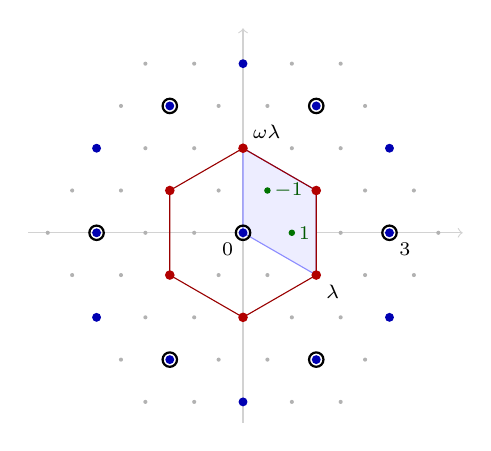
\begin{tikzpicture}[scale=0.62]
\draw[gray!35,->] (-4.40,0)--(4.50,0); \draw[gray!35,->] (0,-3.89)--(0,4.19);
\fill[blue!7] (0.0000,0.0000)--(1.5000,-0.8660)--(1.5000,0.8660)--(0.0000,1.7321)--cycle;
\draw[blue!45] (0.0000,0.0000)--(1.5000,-0.8660)--(1.5000,0.8660)--(0.0000,1.7321)--cycle;
\draw[red!60!black,thin] (-1.5000,-0.8660)--(0.0000,-1.7321)--(1.5000,-0.8660)--(1.5000,0.8660)--(0.0000,1.7321)--(-1.5000,0.8660)--cycle;
\fill[gray!60] (-2.0000,-3.4641) circle (1.2pt);
\fill[gray!60] (-2.5000,-2.5981) circle (1.2pt);
\fill[gray!60] (-3.5000,-0.8660) circle (1.2pt);
\fill[gray!60] (-4.0000,0.0000) circle (1.2pt);
\fill[gray!60] (-1.0000,-3.4641) circle (1.2pt);
\fill[gray!60] (-2.0000,-1.7321) circle (1.2pt);
\fill[gray!60] (-2.5000,-0.8660) circle (1.2pt);
\fill[gray!60] (-3.5000,0.8660) circle (1.2pt);
\fill[gray!60] (-0.5000,-2.5981) circle (1.2pt);
\fill[gray!60] (-1.0000,-1.7321) circle (1.2pt);
\fill[gray!60] (-2.0000,0.0000) circle (1.2pt);
\fill[gray!60] (-2.5000,0.8660) circle (1.2pt);
\fill[gray!60] (1.0000,-3.4641) circle (1.2pt);
\fill[gray!60] (0.5000,-2.5981) circle (1.2pt);
\fill[gray!60] (-0.5000,-0.8660) circle (1.2pt);
\fill[gray!60] (-1.0000,0.0000) circle (1.2pt);
\fill[gray!60] (-2.0000,1.7321) circle (1.2pt);
\fill[gray!60] (-2.5000,2.5981) circle (1.2pt);
\fill[gray!60] (2.0000,-3.4641) circle (1.2pt);
\fill[gray!60] (1.0000,-1.7321) circle (1.2pt);
\fill[gray!60] (0.5000,-0.8660) circle (1.2pt);
\fill[gray!60] (-0.5000,0.8660) circle (1.2pt);
\fill[gray!60] (-1.0000,1.7321) circle (1.2pt);
\fill[gray!60] (-2.0000,3.4641) circle (1.2pt);
\fill[gray!60] (2.5000,-2.5981) circle (1.2pt);
\fill[gray!60] (2.0000,-1.7321) circle (1.2pt);
\fill[gray!60] (1.0000,0.0000) circle (1.2pt);
\fill[gray!60] (0.5000,0.8660) circle (1.2pt);
\fill[gray!60] (-0.5000,2.5981) circle (1.2pt);
\fill[gray!60] (-1.0000,3.4641) circle (1.2pt);
\fill[gray!60] (2.5000,-0.8660) circle (1.2pt);
\fill[gray!60] (2.0000,0.0000) circle (1.2pt);
\fill[gray!60] (1.0000,1.7321) circle (1.2pt);
\fill[gray!60] (0.5000,2.5981) circle (1.2pt);
\fill[gray!60] (3.5000,-0.8660) circle (1.2pt);
\fill[gray!60] (2.5000,0.8660) circle (1.2pt);
\fill[gray!60] (2.0000,1.7321) circle (1.2pt);
\fill[gray!60] (1.0000,3.4641) circle (1.2pt);
\fill[gray!60] (4.0000,0.0000) circle (1.2pt);
\fill[gray!60] (3.5000,0.8660) circle (1.2pt);
\fill[gray!60] (2.5000,2.5981) circle (1.2pt);
\fill[gray!60] (2.0000,3.4641) circle (1.2pt);
\fill[blue!70!black] (-3.0000,-1.7321) circle (2.6pt);
\fill[blue!70!black] (-1.5000,-2.5981) circle (2.6pt);
\fill[blue!70!black] (-3.0000,0.0000) circle (2.6pt);
\fill[blue!70!black] (0.0000,-3.4641) circle (2.6pt);
\fill[blue!70!black] (-3.0000,1.7321) circle (2.6pt);
\fill[blue!70!black] (1.5000,-2.5981) circle (2.6pt);
\fill[blue!70!black] (0.0000,0.0000) circle (2.6pt);
\fill[blue!70!black] (-1.5000,2.5981) circle (2.6pt);
\fill[blue!70!black] (3.0000,-1.7321) circle (2.6pt);
\fill[blue!70!black] (0.0000,3.4641) circle (2.6pt);
\fill[blue!70!black] (3.0000,0.0000) circle (2.6pt);
\fill[blue!70!black] (1.5000,2.5981) circle (2.6pt);
\fill[blue!70!black] (3.0000,1.7321) circle (2.6pt);
\fill[red!70!black] (1.5000,-0.8660) circle (2.8pt);
\fill[red!70!black] (1.5000,0.8660) circle (2.8pt);
\fill[red!70!black] (0.0000,1.7321) circle (2.8pt);
\fill[red!70!black] (-1.5000,0.8660) circle (2.8pt);
\fill[red!70!black] (-1.5000,-0.8660) circle (2.8pt);
\fill[red!70!black] (0.0000,-1.7321) circle (2.8pt);
\draw[black,thick] (-1.5000,-2.5981) circle (4.2pt);
\draw[black,thick] (-3.0000,0.0000) circle (4.2pt);
\draw[black,thick] (1.5000,-2.5981) circle (4.2pt);
\draw[black,thick] (0.0000,0.0000) circle (4.2pt);
\draw[black,thick] (-1.5000,2.5981) circle (4.2pt);
\draw[black,thick] (3.0000,0.0000) circle (4.2pt);
\draw[black,thick] (1.5000,2.5981) circle (4.2pt);
\fill[green!45!black] (1.0000,0.0000) circle (1.9pt);
\fill[green!45!black] (0.5000,0.8660) circle (1.9pt);
\node[right=-1pt,font=\scriptsize,green!35!black] at (1.0000,0.0000) {$1$};
\node[right=-1pt,font=\scriptsize,green!35!black] at (0.5000,0.8660) {$-1$};
\node[below left,font=\scriptsize] at (0.0000,0.0000) {$0$};
\node[below right,font=\scriptsize] at (1.5000,-0.8660) {$\lambda$};
\node[below right,font=\scriptsize] at (3.0000,0.0000) {$3$};
\node[above right,font=\scriptsize] at (0.0000,1.7321) {$\omega\lambda$};
\end{tikzpicture}
\hfill
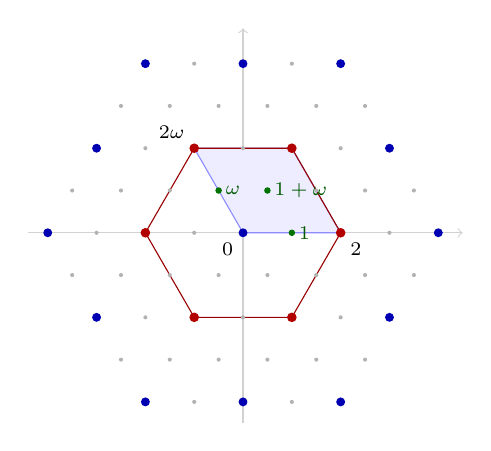
\begin{tikzpicture}[scale=0.62]
\draw[gray!35,->] (-4.40,0)--(4.50,0); \draw[gray!35,->] (0,-3.89)--(0,4.19);
\fill[blue!7] (0.0000,0.0000)--(2.0000,0.0000)--(1.0000,1.7321)--(-1.0000,1.7321)--cycle;
\draw[blue!45] (0.0000,0.0000)--(2.0000,0.0000)--(1.0000,1.7321)--(-1.0000,1.7321)--cycle;
\draw[red!60!black,thin] (-1.0000,-1.7321)--(1.0000,-1.7321)--(2.0000,0.0000)--(1.0000,1.7321)--(-1.0000,1.7321)--(-2.0000,0.0000)--cycle;
\fill[gray!60] (-2.5000,-2.5981) circle (1.2pt);
\fill[gray!60] (-3.5000,-0.8660) circle (1.2pt);
\fill[gray!60] (-1.0000,-3.4641) circle (1.2pt);
\fill[gray!60] (-1.5000,-2.5981) circle (1.2pt);
\fill[gray!60] (-2.0000,-1.7321) circle (1.2pt);
\fill[gray!60] (-2.5000,-0.8660) circle (1.2pt);
\fill[gray!60] (-3.0000,0.0000) circle (1.2pt);
\fill[gray!60] (-3.5000,0.8660) circle (1.2pt);
\fill[gray!60] (-0.5000,-2.5981) circle (1.2pt);
\fill[gray!60] (-1.5000,-0.8660) circle (1.2pt);
\fill[gray!60] (-2.5000,0.8660) circle (1.2pt);
\fill[gray!60] (1.0000,-3.4641) circle (1.2pt);
\fill[gray!60] (0.5000,-2.5981) circle (1.2pt);
\fill[gray!60] (0.0000,-1.7321) circle (1.2pt);
\fill[gray!60] (-0.5000,-0.8660) circle (1.2pt);
\fill[gray!60] (-1.0000,0.0000) circle (1.2pt);
\fill[gray!60] (-1.5000,0.8660) circle (1.2pt);
\fill[gray!60] (-2.0000,1.7321) circle (1.2pt);
\fill[gray!60] (-2.5000,2.5981) circle (1.2pt);
\fill[gray!60] (1.5000,-2.5981) circle (1.2pt);
\fill[gray!60] (0.5000,-0.8660) circle (1.2pt);
\fill[gray!60] (-0.5000,0.8660) circle (1.2pt);
\fill[gray!60] (-1.5000,2.5981) circle (1.2pt);
\fill[gray!60] (2.5000,-2.5981) circle (1.2pt);
\fill[gray!60] (2.0000,-1.7321) circle (1.2pt);
\fill[gray!60] (1.5000,-0.8660) circle (1.2pt);
\fill[gray!60] (1.0000,0.0000) circle (1.2pt);
\fill[gray!60] (0.5000,0.8660) circle (1.2pt);
\fill[gray!60] (0.0000,1.7321) circle (1.2pt);
\fill[gray!60] (-0.5000,2.5981) circle (1.2pt);
\fill[gray!60] (-1.0000,3.4641) circle (1.2pt);
\fill[gray!60] (2.5000,-0.8660) circle (1.2pt);
\fill[gray!60] (1.5000,0.8660) circle (1.2pt);
\fill[gray!60] (0.5000,2.5981) circle (1.2pt);
\fill[gray!60] (3.5000,-0.8660) circle (1.2pt);
\fill[gray!60] (3.0000,0.0000) circle (1.2pt);
\fill[gray!60] (2.5000,0.8660) circle (1.2pt);
\fill[gray!60] (2.0000,1.7321) circle (1.2pt);
\fill[gray!60] (1.5000,2.5981) circle (1.2pt);
\fill[gray!60] (1.0000,3.4641) circle (1.2pt);
\fill[gray!60] (3.5000,0.8660) circle (1.2pt);
\fill[gray!60] (2.5000,2.5981) circle (1.2pt);
\fill[blue!70!black] (-2.0000,-3.4641) circle (2.6pt);
\fill[blue!70!black] (-3.0000,-1.7321) circle (2.6pt);
\fill[blue!70!black] (-4.0000,0.0000) circle (2.6pt);
\fill[blue!70!black] (0.0000,-3.4641) circle (2.6pt);
\fill[blue!70!black] (-3.0000,1.7321) circle (2.6pt);
\fill[blue!70!black] (2.0000,-3.4641) circle (2.6pt);
\fill[blue!70!black] (0.0000,0.0000) circle (2.6pt);
\fill[blue!70!black] (-2.0000,3.4641) circle (2.6pt);
\fill[blue!70!black] (3.0000,-1.7321) circle (2.6pt);
\fill[blue!70!black] (0.0000,3.4641) circle (2.6pt);
\fill[blue!70!black] (4.0000,0.0000) circle (2.6pt);
\fill[blue!70!black] (3.0000,1.7321) circle (2.6pt);
\fill[blue!70!black] (2.0000,3.4641) circle (2.6pt);
\fill[red!70!black] (2.0000,0.0000) circle (2.8pt);
\fill[red!70!black] (1.0000,1.7321) circle (2.8pt);
\fill[red!70!black] (-1.0000,1.7321) circle (2.8pt);
\fill[red!70!black] (-2.0000,0.0000) circle (2.8pt);
\fill[red!70!black] (-1.0000,-1.7321) circle (2.8pt);
\fill[red!70!black] (1.0000,-1.7321) circle (2.8pt);
\fill[green!45!black] (-0.5000,0.8660) circle (1.9pt);
\fill[green!45!black] (1.0000,0.0000) circle (1.9pt);
\fill[green!45!black] (0.5000,0.8660) circle (1.9pt);
\node[right=-1pt,font=\scriptsize,green!35!black] at (-0.5000,0.8660) {$\omega$};
\node[right=-1pt,font=\scriptsize,green!35!black] at (1.0000,0.0000) {$1$};
\node[right=-1pt,font=\scriptsize,green!35!black] at (0.5000,0.8660) {$1+\omega$};
\node[below left,font=\scriptsize] at (0.0000,0.0000) {$0$};
\node[below right,font=\scriptsize] at (2.0000,0.0000) {$2$};
\node[above left,font=\scriptsize] at (-1.0000,1.7321) {$2\omega$};
\end{tikzpicture}

\caption{Left: the ramified prime $(\lambda)=I_{3,1}=\{x+y\omega:3\mid x+y\}$ of norm $3$. Its six generators
$\pm\lambda,\pm\omega\lambda,\pm\omega^2\lambda$ (red) form a hexagon turned by $30^\circ$ relative to the units,
and the parallelogram spanned by $\lambda$ and $\omega\lambda$ contains one point of each class of
$\OO/\lambda\cong\F_3$ ($0$ and the green points), labelled by $x+y\bmod3$. Black rings mark $(\lambda)^2=(3)$, of index $3$ in $(\lambda)$.
Right: the inert prime $(2)=2\OO$ of norm $4$, a copy of $\OO$ scaled by $2$. The parallelogram spanned by $2$ and
$2\omega$ contains the residues $0,1,\omega,1+\omega$, which represent $\OO/2\cong\F_4$ (note $1+\omega=-\omega^2\equiv\omega^2$).}
\label{fig:ideal-ram-inert}
\end{figure}

\begin{figure}[ht]
\centering
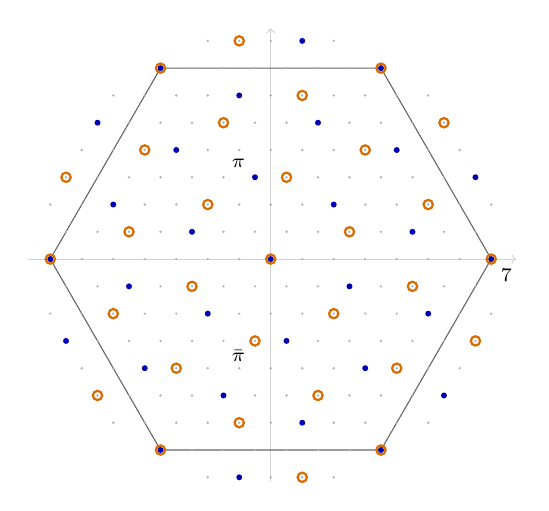
\begin{tikzpicture}[scale=0.4]
\draw[gray!35,->] (-7.70,0)--(7.80,0); \draw[gray!35,->] (0,-7.03)--(0,7.33);
\draw[black!60,thin] (-3.5000,-6.0622)--(3.5000,-6.0622)--(7.0000,0.0000)--(3.5000,6.0622)--(-3.5000,6.0622)--(-7.0000,0.0000)--cycle;
\fill[gray!60] (-5.0000,-5.1962) circle (1.2pt);
\fill[gray!60] (-5.5000,-4.3301) circle (1.2pt);
\fill[gray!60] (-6.0000,-3.4641) circle (1.2pt);
\fill[gray!60] (-7.0000,-1.7321) circle (1.2pt);
\fill[gray!60] (-4.0000,-5.1962) circle (1.2pt);
\fill[gray!60] (-4.5000,-4.3301) circle (1.2pt);
\fill[gray!60] (-5.0000,-3.4641) circle (1.2pt);
\fill[gray!60] (-5.5000,-2.5981) circle (1.2pt);
\fill[gray!60] (-6.0000,-1.7321) circle (1.2pt);
\fill[gray!60] (-6.5000,-0.8660) circle (1.2pt);
\fill[gray!60] (-2.0000,-6.9282) circle (1.2pt);
\fill[gray!60] (-2.5000,-6.0622) circle (1.2pt);
\fill[gray!60] (-3.0000,-5.1962) circle (1.2pt);
\fill[gray!60] (-3.5000,-4.3301) circle (1.2pt);
\fill[gray!60] (-4.5000,-2.5981) circle (1.2pt);
\fill[gray!60] (-5.0000,-1.7321) circle (1.2pt);
\fill[gray!60] (-5.5000,-0.8660) circle (1.2pt);
\fill[gray!60] (-6.0000,0.0000) circle (1.2pt);
\fill[gray!60] (-6.5000,0.8660) circle (1.2pt);
\fill[gray!60] (-7.0000,1.7321) circle (1.2pt);
\fill[gray!60] (-1.5000,-6.0622) circle (1.2pt);
\fill[gray!60] (-2.0000,-5.1962) circle (1.2pt);
\fill[gray!60] (-2.5000,-4.3301) circle (1.2pt);
\fill[gray!60] (-3.0000,-3.4641) circle (1.2pt);
\fill[gray!60] (-3.5000,-2.5981) circle (1.2pt);
\fill[gray!60] (-4.0000,-1.7321) circle (1.2pt);
\fill[gray!60] (-5.0000,0.0000) circle (1.2pt);
\fill[gray!60] (-5.5000,0.8660) circle (1.2pt);
\fill[gray!60] (-6.0000,1.7321) circle (1.2pt);
\fill[gray!60] (-6.5000,2.5981) circle (1.2pt);
\fill[gray!60] (0.0000,-6.9282) circle (1.2pt);
\fill[gray!60] (-0.5000,-6.0622) circle (1.2pt);
\fill[gray!60] (-1.0000,-5.1962) circle (1.2pt);
\fill[gray!60] (-2.0000,-3.4641) circle (1.2pt);
\fill[gray!60] (-2.5000,-2.5981) circle (1.2pt);
\fill[gray!60] (-3.0000,-1.7321) circle (1.2pt);
\fill[gray!60] (-3.5000,-0.8660) circle (1.2pt);
\fill[gray!60] (-4.0000,0.0000) circle (1.2pt);
\fill[gray!60] (-4.5000,0.8660) circle (1.2pt);
\fill[gray!60] (-5.5000,2.5981) circle (1.2pt);
\fill[gray!60] (-6.0000,3.4641) circle (1.2pt);
\fill[gray!60] (1.0000,-6.9282) circle (1.2pt);
\fill[gray!60] (0.5000,-6.0622) circle (1.2pt);
\fill[gray!60] (0.0000,-5.1962) circle (1.2pt);
\fill[gray!60] (-0.5000,-4.3301) circle (1.2pt);
\fill[gray!60] (-1.0000,-3.4641) circle (1.2pt);
\fill[gray!60] (-1.5000,-2.5981) circle (1.2pt);
\fill[gray!60] (-2.5000,-0.8660) circle (1.2pt);
\fill[gray!60] (-3.0000,0.0000) circle (1.2pt);
\fill[gray!60] (-3.5000,0.8660) circle (1.2pt);
\fill[gray!60] (-4.0000,1.7321) circle (1.2pt);
\fill[gray!60] (-4.5000,2.5981) circle (1.2pt);
\fill[gray!60] (-5.0000,3.4641) circle (1.2pt);
\fill[gray!60] (2.0000,-6.9282) circle (1.2pt);
\fill[gray!60] (1.5000,-6.0622) circle (1.2pt);
\fill[gray!60] (0.5000,-4.3301) circle (1.2pt);
\fill[gray!60] (0.0000,-3.4641) circle (1.2pt);
\fill[gray!60] (-0.5000,-2.5981) circle (1.2pt);
\fill[gray!60] (-1.0000,-1.7321) circle (1.2pt);
\fill[gray!60] (-1.5000,-0.8660) circle (1.2pt);
\fill[gray!60] (-2.0000,0.0000) circle (1.2pt);
\fill[gray!60] (-3.0000,1.7321) circle (1.2pt);
\fill[gray!60] (-3.5000,2.5981) circle (1.2pt);
\fill[gray!60] (-4.0000,3.4641) circle (1.2pt);
\fill[gray!60] (-4.5000,4.3301) circle (1.2pt);
\fill[gray!60] (-5.0000,5.1962) circle (1.2pt);
\fill[gray!60] (2.5000,-6.0622) circle (1.2pt);
\fill[gray!60] (2.0000,-5.1962) circle (1.2pt);
\fill[gray!60] (1.5000,-4.3301) circle (1.2pt);
\fill[gray!60] (1.0000,-3.4641) circle (1.2pt);
\fill[gray!60] (0.0000,-1.7321) circle (1.2pt);
\fill[gray!60] (-0.5000,-0.8660) circle (1.2pt);
\fill[gray!60] (-1.0000,0.0000) circle (1.2pt);
\fill[gray!60] (-1.5000,0.8660) circle (1.2pt);
\fill[gray!60] (-2.0000,1.7321) circle (1.2pt);
\fill[gray!60] (-2.5000,2.5981) circle (1.2pt);
\fill[gray!60] (-3.5000,4.3301) circle (1.2pt);
\fill[gray!60] (-4.0000,5.1962) circle (1.2pt);
\fill[gray!60] (3.0000,-5.1962) circle (1.2pt);
\fill[gray!60] (2.5000,-4.3301) circle (1.2pt);
\fill[gray!60] (2.0000,-3.4641) circle (1.2pt);
\fill[gray!60] (1.5000,-2.5981) circle (1.2pt);
\fill[gray!60] (1.0000,-1.7321) circle (1.2pt);
\fill[gray!60] (0.5000,-0.8660) circle (1.2pt);
\fill[gray!60] (-0.5000,0.8660) circle (1.2pt);
\fill[gray!60] (-1.0000,1.7321) circle (1.2pt);
\fill[gray!60] (-1.5000,2.5981) circle (1.2pt);
\fill[gray!60] (-2.0000,3.4641) circle (1.2pt);
\fill[gray!60] (-2.5000,4.3301) circle (1.2pt);
\fill[gray!60] (-3.0000,5.1962) circle (1.2pt);
\fill[gray!60] (4.0000,-5.1962) circle (1.2pt);
\fill[gray!60] (3.5000,-4.3301) circle (1.2pt);
\fill[gray!60] (2.5000,-2.5981) circle (1.2pt);
\fill[gray!60] (2.0000,-1.7321) circle (1.2pt);
\fill[gray!60] (1.5000,-0.8660) circle (1.2pt);
\fill[gray!60] (1.0000,0.0000) circle (1.2pt);
\fill[gray!60] (0.5000,0.8660) circle (1.2pt);
\fill[gray!60] (0.0000,1.7321) circle (1.2pt);
\fill[gray!60] (-1.0000,3.4641) circle (1.2pt);
\fill[gray!60] (-1.5000,4.3301) circle (1.2pt);
\fill[gray!60] (-2.0000,5.1962) circle (1.2pt);
\fill[gray!60] (-2.5000,6.0622) circle (1.2pt);
\fill[gray!60] (5.0000,-5.1962) circle (1.2pt);
\fill[gray!60] (4.5000,-4.3301) circle (1.2pt);
\fill[gray!60] (4.0000,-3.4641) circle (1.2pt);
\fill[gray!60] (3.5000,-2.5981) circle (1.2pt);
\fill[gray!60] (3.0000,-1.7321) circle (1.2pt);
\fill[gray!60] (2.0000,0.0000) circle (1.2pt);
\fill[gray!60] (1.5000,0.8660) circle (1.2pt);
\fill[gray!60] (1.0000,1.7321) circle (1.2pt);
\fill[gray!60] (0.5000,2.5981) circle (1.2pt);
\fill[gray!60] (0.0000,3.4641) circle (1.2pt);
\fill[gray!60] (-0.5000,4.3301) circle (1.2pt);
\fill[gray!60] (-1.5000,6.0622) circle (1.2pt);
\fill[gray!60] (-2.0000,6.9282) circle (1.2pt);
\fill[gray!60] (5.0000,-3.4641) circle (1.2pt);
\fill[gray!60] (4.5000,-2.5981) circle (1.2pt);
\fill[gray!60] (4.0000,-1.7321) circle (1.2pt);
\fill[gray!60] (3.5000,-0.8660) circle (1.2pt);
\fill[gray!60] (3.0000,0.0000) circle (1.2pt);
\fill[gray!60] (2.5000,0.8660) circle (1.2pt);
\fill[gray!60] (1.5000,2.5981) circle (1.2pt);
\fill[gray!60] (1.0000,3.4641) circle (1.2pt);
\fill[gray!60] (0.5000,4.3301) circle (1.2pt);
\fill[gray!60] (0.0000,5.1962) circle (1.2pt);
\fill[gray!60] (-0.5000,6.0622) circle (1.2pt);
\fill[gray!60] (-1.0000,6.9282) circle (1.2pt);
\fill[gray!60] (6.0000,-3.4641) circle (1.2pt);
\fill[gray!60] (5.5000,-2.5981) circle (1.2pt);
\fill[gray!60] (4.5000,-0.8660) circle (1.2pt);
\fill[gray!60] (4.0000,0.0000) circle (1.2pt);
\fill[gray!60] (3.5000,0.8660) circle (1.2pt);
\fill[gray!60] (3.0000,1.7321) circle (1.2pt);
\fill[gray!60] (2.5000,2.5981) circle (1.2pt);
\fill[gray!60] (2.0000,3.4641) circle (1.2pt);
\fill[gray!60] (1.0000,5.1962) circle (1.2pt);
\fill[gray!60] (0.5000,6.0622) circle (1.2pt);
\fill[gray!60] (0.0000,6.9282) circle (1.2pt);
\fill[gray!60] (6.5000,-2.5981) circle (1.2pt);
\fill[gray!60] (6.0000,-1.7321) circle (1.2pt);
\fill[gray!60] (5.5000,-0.8660) circle (1.2pt);
\fill[gray!60] (5.0000,0.0000) circle (1.2pt);
\fill[gray!60] (4.0000,1.7321) circle (1.2pt);
\fill[gray!60] (3.5000,2.5981) circle (1.2pt);
\fill[gray!60] (3.0000,3.4641) circle (1.2pt);
\fill[gray!60] (2.5000,4.3301) circle (1.2pt);
\fill[gray!60] (2.0000,5.1962) circle (1.2pt);
\fill[gray!60] (1.5000,6.0622) circle (1.2pt);
\fill[gray!60] (7.0000,-1.7321) circle (1.2pt);
\fill[gray!60] (6.5000,-0.8660) circle (1.2pt);
\fill[gray!60] (6.0000,0.0000) circle (1.2pt);
\fill[gray!60] (5.5000,0.8660) circle (1.2pt);
\fill[gray!60] (5.0000,1.7321) circle (1.2pt);
\fill[gray!60] (4.5000,2.5981) circle (1.2pt);
\fill[gray!60] (3.5000,4.3301) circle (1.2pt);
\fill[gray!60] (3.0000,5.1962) circle (1.2pt);
\fill[gray!60] (2.5000,6.0622) circle (1.2pt);
\fill[gray!60] (2.0000,6.9282) circle (1.2pt);
\fill[gray!60] (6.5000,0.8660) circle (1.2pt);
\fill[gray!60] (6.0000,1.7321) circle (1.2pt);
\fill[gray!60] (5.5000,2.5981) circle (1.2pt);
\fill[gray!60] (5.0000,3.4641) circle (1.2pt);
\fill[gray!60] (4.5000,4.3301) circle (1.2pt);
\fill[gray!60] (4.0000,5.1962) circle (1.2pt);
\fill[gray!60] (7.0000,1.7321) circle (1.2pt);
\fill[gray!60] (6.0000,3.4641) circle (1.2pt);
\fill[gray!60] (5.5000,4.3301) circle (1.2pt);
\fill[gray!60] (5.0000,5.1962) circle (1.2pt);
\fill[blue!70!black] (-6.5000,-2.5981) circle (2.7pt);
\fill[blue!70!black] (-3.5000,-6.0622) circle (2.7pt);
\fill[blue!70!black] (-7.0000,0.0000) circle (2.7pt);
\fill[blue!70!black] (-4.0000,-3.4641) circle (2.7pt);
\fill[blue!70!black] (-1.0000,-6.9282) circle (2.7pt);
\fill[blue!70!black] (-4.5000,-0.8660) circle (2.7pt);
\fill[blue!70!black] (-1.5000,-4.3301) circle (2.7pt);
\fill[blue!70!black] (-5.0000,1.7321) circle (2.7pt);
\fill[blue!70!black] (-2.0000,-1.7321) circle (2.7pt);
\fill[blue!70!black] (-5.5000,4.3301) circle (2.7pt);
\fill[blue!70!black] (1.0000,-5.1962) circle (2.7pt);
\fill[blue!70!black] (-2.5000,0.8660) circle (2.7pt);
\fill[blue!70!black] (0.5000,-2.5981) circle (2.7pt);
\fill[blue!70!black] (-3.0000,3.4641) circle (2.7pt);
\fill[blue!70!black] (3.5000,-6.0622) circle (2.7pt);
\fill[blue!70!black] (0.0000,0.0000) circle (2.7pt);
\fill[blue!70!black] (-3.5000,6.0622) circle (2.7pt);
\fill[blue!70!black] (3.0000,-3.4641) circle (2.7pt);
\fill[blue!70!black] (-0.5000,2.5981) circle (2.7pt);
\fill[blue!70!black] (2.5000,-0.8660) circle (2.7pt);
\fill[blue!70!black] (-1.0000,5.1962) circle (2.7pt);
\fill[blue!70!black] (5.5000,-4.3301) circle (2.7pt);
\fill[blue!70!black] (2.0000,1.7321) circle (2.7pt);
\fill[blue!70!black] (5.0000,-1.7321) circle (2.7pt);
\fill[blue!70!black] (1.5000,4.3301) circle (2.7pt);
\fill[blue!70!black] (4.5000,0.8660) circle (2.7pt);
\fill[blue!70!black] (1.0000,6.9282) circle (2.7pt);
\fill[blue!70!black] (4.0000,3.4641) circle (2.7pt);
\fill[blue!70!black] (7.0000,0.0000) circle (2.7pt);
\fill[blue!70!black] (3.5000,6.0622) circle (2.7pt);
\fill[blue!70!black] (6.5000,2.5981) circle (2.7pt);
\draw[orange!85!black,thick] (-5.5000,-4.3301) circle (4.2pt);
\draw[orange!85!black,thick] (-3.5000,-6.0622) circle (4.2pt);
\draw[orange!85!black,thick] (-7.0000,0.0000) circle (4.2pt);
\draw[orange!85!black,thick] (-5.0000,-1.7321) circle (4.2pt);
\draw[orange!85!black,thick] (-3.0000,-3.4641) circle (4.2pt);
\draw[orange!85!black,thick] (-6.5000,2.5981) circle (4.2pt);
\draw[orange!85!black,thick] (-1.0000,-5.1962) circle (4.2pt);
\draw[orange!85!black,thick] (-4.5000,0.8660) circle (4.2pt);
\draw[orange!85!black,thick] (1.0000,-6.9282) circle (4.2pt);
\draw[orange!85!black,thick] (-2.5000,-0.8660) circle (4.2pt);
\draw[orange!85!black,thick] (-0.5000,-2.5981) circle (4.2pt);
\draw[orange!85!black,thick] (-4.0000,3.4641) circle (4.2pt);
\draw[orange!85!black,thick] (1.5000,-4.3301) circle (4.2pt);
\draw[orange!85!black,thick] (-2.0000,1.7321) circle (4.2pt);
\draw[orange!85!black,thick] (3.5000,-6.0622) circle (4.2pt);
\draw[orange!85!black,thick] (0.0000,0.0000) circle (4.2pt);
\draw[orange!85!black,thick] (-3.5000,6.0622) circle (4.2pt);
\draw[orange!85!black,thick] (2.0000,-1.7321) circle (4.2pt);
\draw[orange!85!black,thick] (-1.5000,4.3301) circle (4.2pt);
\draw[orange!85!black,thick] (4.0000,-3.4641) circle (4.2pt);
\draw[orange!85!black,thick] (0.5000,2.5981) circle (4.2pt);
\draw[orange!85!black,thick] (2.5000,0.8660) circle (4.2pt);
\draw[orange!85!black,thick] (-1.0000,6.9282) circle (4.2pt);
\draw[orange!85!black,thick] (4.5000,-0.8660) circle (4.2pt);
\draw[orange!85!black,thick] (1.0000,5.1962) circle (4.2pt);
\draw[orange!85!black,thick] (6.5000,-2.5981) circle (4.2pt);
\draw[orange!85!black,thick] (3.0000,3.4641) circle (4.2pt);
\draw[orange!85!black,thick] (5.0000,1.7321) circle (4.2pt);
\draw[orange!85!black,thick] (7.0000,0.0000) circle (4.2pt);
\draw[orange!85!black,thick] (3.5000,6.0622) circle (4.2pt);
\draw[orange!85!black,thick] (5.5000,4.3301) circle (4.2pt);
\node[above left,font=\scriptsize] at (-0.5000,2.5981) {$\pi$};
\node[below left,font=\scriptsize] at (-0.5000,-2.5981) {$\bar\pi$};
\node[below right,font=\scriptsize] at (7.0000,0.0000) {$7$};
\end{tikzpicture}
\hfill
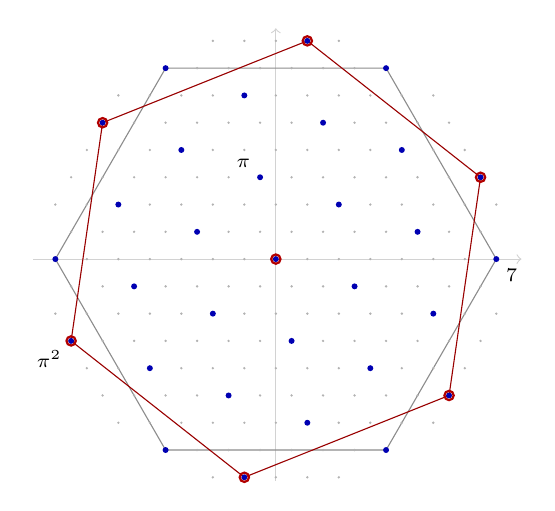
\begin{tikzpicture}[scale=0.4]
\draw[gray!35,->] (-7.70,0)--(7.80,0); \draw[gray!35,->] (0,-7.03)--(0,7.33);
\draw[black!45,thin] (-3.5000,-6.0622)--(3.5000,-6.0622)--(7.0000,0.0000)--(3.5000,6.0622)--(-3.5000,6.0622)--(-7.0000,0.0000)--cycle;
\draw[red!60!black,thin] (-6.5000,-2.5981)--(-1.0000,-6.9282)--(5.5000,-4.3301)--(6.5000,2.5981)--(1.0000,6.9282)--(-5.5000,4.3301)--cycle;
\fill[gray!60] (-5.0000,-5.1962) circle (1.2pt);
\fill[gray!60] (-5.5000,-4.3301) circle (1.2pt);
\fill[gray!60] (-6.0000,-3.4641) circle (1.2pt);
\fill[gray!60] (-7.0000,-1.7321) circle (1.2pt);
\fill[gray!60] (-4.0000,-5.1962) circle (1.2pt);
\fill[gray!60] (-4.5000,-4.3301) circle (1.2pt);
\fill[gray!60] (-5.0000,-3.4641) circle (1.2pt);
\fill[gray!60] (-5.5000,-2.5981) circle (1.2pt);
\fill[gray!60] (-6.0000,-1.7321) circle (1.2pt);
\fill[gray!60] (-6.5000,-0.8660) circle (1.2pt);
\fill[gray!60] (-2.0000,-6.9282) circle (1.2pt);
\fill[gray!60] (-2.5000,-6.0622) circle (1.2pt);
\fill[gray!60] (-3.0000,-5.1962) circle (1.2pt);
\fill[gray!60] (-3.5000,-4.3301) circle (1.2pt);
\fill[gray!60] (-4.5000,-2.5981) circle (1.2pt);
\fill[gray!60] (-5.0000,-1.7321) circle (1.2pt);
\fill[gray!60] (-5.5000,-0.8660) circle (1.2pt);
\fill[gray!60] (-6.0000,0.0000) circle (1.2pt);
\fill[gray!60] (-6.5000,0.8660) circle (1.2pt);
\fill[gray!60] (-7.0000,1.7321) circle (1.2pt);
\fill[gray!60] (-1.5000,-6.0622) circle (1.2pt);
\fill[gray!60] (-2.0000,-5.1962) circle (1.2pt);
\fill[gray!60] (-2.5000,-4.3301) circle (1.2pt);
\fill[gray!60] (-3.0000,-3.4641) circle (1.2pt);
\fill[gray!60] (-3.5000,-2.5981) circle (1.2pt);
\fill[gray!60] (-4.0000,-1.7321) circle (1.2pt);
\fill[gray!60] (-5.0000,0.0000) circle (1.2pt);
\fill[gray!60] (-5.5000,0.8660) circle (1.2pt);
\fill[gray!60] (-6.0000,1.7321) circle (1.2pt);
\fill[gray!60] (-6.5000,2.5981) circle (1.2pt);
\fill[gray!60] (0.0000,-6.9282) circle (1.2pt);
\fill[gray!60] (-0.5000,-6.0622) circle (1.2pt);
\fill[gray!60] (-1.0000,-5.1962) circle (1.2pt);
\fill[gray!60] (-2.0000,-3.4641) circle (1.2pt);
\fill[gray!60] (-2.5000,-2.5981) circle (1.2pt);
\fill[gray!60] (-3.0000,-1.7321) circle (1.2pt);
\fill[gray!60] (-3.5000,-0.8660) circle (1.2pt);
\fill[gray!60] (-4.0000,0.0000) circle (1.2pt);
\fill[gray!60] (-4.5000,0.8660) circle (1.2pt);
\fill[gray!60] (-5.5000,2.5981) circle (1.2pt);
\fill[gray!60] (-6.0000,3.4641) circle (1.2pt);
\fill[gray!60] (1.0000,-6.9282) circle (1.2pt);
\fill[gray!60] (0.5000,-6.0622) circle (1.2pt);
\fill[gray!60] (0.0000,-5.1962) circle (1.2pt);
\fill[gray!60] (-0.5000,-4.3301) circle (1.2pt);
\fill[gray!60] (-1.0000,-3.4641) circle (1.2pt);
\fill[gray!60] (-1.5000,-2.5981) circle (1.2pt);
\fill[gray!60] (-2.5000,-0.8660) circle (1.2pt);
\fill[gray!60] (-3.0000,0.0000) circle (1.2pt);
\fill[gray!60] (-3.5000,0.8660) circle (1.2pt);
\fill[gray!60] (-4.0000,1.7321) circle (1.2pt);
\fill[gray!60] (-4.5000,2.5981) circle (1.2pt);
\fill[gray!60] (-5.0000,3.4641) circle (1.2pt);
\fill[gray!60] (2.0000,-6.9282) circle (1.2pt);
\fill[gray!60] (1.5000,-6.0622) circle (1.2pt);
\fill[gray!60] (0.5000,-4.3301) circle (1.2pt);
\fill[gray!60] (0.0000,-3.4641) circle (1.2pt);
\fill[gray!60] (-0.5000,-2.5981) circle (1.2pt);
\fill[gray!60] (-1.0000,-1.7321) circle (1.2pt);
\fill[gray!60] (-1.5000,-0.8660) circle (1.2pt);
\fill[gray!60] (-2.0000,0.0000) circle (1.2pt);
\fill[gray!60] (-3.0000,1.7321) circle (1.2pt);
\fill[gray!60] (-3.5000,2.5981) circle (1.2pt);
\fill[gray!60] (-4.0000,3.4641) circle (1.2pt);
\fill[gray!60] (-4.5000,4.3301) circle (1.2pt);
\fill[gray!60] (-5.0000,5.1962) circle (1.2pt);
\fill[gray!60] (2.5000,-6.0622) circle (1.2pt);
\fill[gray!60] (2.0000,-5.1962) circle (1.2pt);
\fill[gray!60] (1.5000,-4.3301) circle (1.2pt);
\fill[gray!60] (1.0000,-3.4641) circle (1.2pt);
\fill[gray!60] (0.0000,-1.7321) circle (1.2pt);
\fill[gray!60] (-0.5000,-0.8660) circle (1.2pt);
\fill[gray!60] (-1.0000,0.0000) circle (1.2pt);
\fill[gray!60] (-1.5000,0.8660) circle (1.2pt);
\fill[gray!60] (-2.0000,1.7321) circle (1.2pt);
\fill[gray!60] (-2.5000,2.5981) circle (1.2pt);
\fill[gray!60] (-3.5000,4.3301) circle (1.2pt);
\fill[gray!60] (-4.0000,5.1962) circle (1.2pt);
\fill[gray!60] (3.0000,-5.1962) circle (1.2pt);
\fill[gray!60] (2.5000,-4.3301) circle (1.2pt);
\fill[gray!60] (2.0000,-3.4641) circle (1.2pt);
\fill[gray!60] (1.5000,-2.5981) circle (1.2pt);
\fill[gray!60] (1.0000,-1.7321) circle (1.2pt);
\fill[gray!60] (0.5000,-0.8660) circle (1.2pt);
\fill[gray!60] (-0.5000,0.8660) circle (1.2pt);
\fill[gray!60] (-1.0000,1.7321) circle (1.2pt);
\fill[gray!60] (-1.5000,2.5981) circle (1.2pt);
\fill[gray!60] (-2.0000,3.4641) circle (1.2pt);
\fill[gray!60] (-2.5000,4.3301) circle (1.2pt);
\fill[gray!60] (-3.0000,5.1962) circle (1.2pt);
\fill[gray!60] (4.0000,-5.1962) circle (1.2pt);
\fill[gray!60] (3.5000,-4.3301) circle (1.2pt);
\fill[gray!60] (2.5000,-2.5981) circle (1.2pt);
\fill[gray!60] (2.0000,-1.7321) circle (1.2pt);
\fill[gray!60] (1.5000,-0.8660) circle (1.2pt);
\fill[gray!60] (1.0000,0.0000) circle (1.2pt);
\fill[gray!60] (0.5000,0.8660) circle (1.2pt);
\fill[gray!60] (0.0000,1.7321) circle (1.2pt);
\fill[gray!60] (-1.0000,3.4641) circle (1.2pt);
\fill[gray!60] (-1.5000,4.3301) circle (1.2pt);
\fill[gray!60] (-2.0000,5.1962) circle (1.2pt);
\fill[gray!60] (-2.5000,6.0622) circle (1.2pt);
\fill[gray!60] (5.0000,-5.1962) circle (1.2pt);
\fill[gray!60] (4.5000,-4.3301) circle (1.2pt);
\fill[gray!60] (4.0000,-3.4641) circle (1.2pt);
\fill[gray!60] (3.5000,-2.5981) circle (1.2pt);
\fill[gray!60] (3.0000,-1.7321) circle (1.2pt);
\fill[gray!60] (2.0000,0.0000) circle (1.2pt);
\fill[gray!60] (1.5000,0.8660) circle (1.2pt);
\fill[gray!60] (1.0000,1.7321) circle (1.2pt);
\fill[gray!60] (0.5000,2.5981) circle (1.2pt);
\fill[gray!60] (0.0000,3.4641) circle (1.2pt);
\fill[gray!60] (-0.5000,4.3301) circle (1.2pt);
\fill[gray!60] (-1.5000,6.0622) circle (1.2pt);
\fill[gray!60] (-2.0000,6.9282) circle (1.2pt);
\fill[gray!60] (5.0000,-3.4641) circle (1.2pt);
\fill[gray!60] (4.5000,-2.5981) circle (1.2pt);
\fill[gray!60] (4.0000,-1.7321) circle (1.2pt);
\fill[gray!60] (3.5000,-0.8660) circle (1.2pt);
\fill[gray!60] (3.0000,0.0000) circle (1.2pt);
\fill[gray!60] (2.5000,0.8660) circle (1.2pt);
\fill[gray!60] (1.5000,2.5981) circle (1.2pt);
\fill[gray!60] (1.0000,3.4641) circle (1.2pt);
\fill[gray!60] (0.5000,4.3301) circle (1.2pt);
\fill[gray!60] (0.0000,5.1962) circle (1.2pt);
\fill[gray!60] (-0.5000,6.0622) circle (1.2pt);
\fill[gray!60] (-1.0000,6.9282) circle (1.2pt);
\fill[gray!60] (6.0000,-3.4641) circle (1.2pt);
\fill[gray!60] (5.5000,-2.5981) circle (1.2pt);
\fill[gray!60] (4.5000,-0.8660) circle (1.2pt);
\fill[gray!60] (4.0000,0.0000) circle (1.2pt);
\fill[gray!60] (3.5000,0.8660) circle (1.2pt);
\fill[gray!60] (3.0000,1.7321) circle (1.2pt);
\fill[gray!60] (2.5000,2.5981) circle (1.2pt);
\fill[gray!60] (2.0000,3.4641) circle (1.2pt);
\fill[gray!60] (1.0000,5.1962) circle (1.2pt);
\fill[gray!60] (0.5000,6.0622) circle (1.2pt);
\fill[gray!60] (0.0000,6.9282) circle (1.2pt);
\fill[gray!60] (6.5000,-2.5981) circle (1.2pt);
\fill[gray!60] (6.0000,-1.7321) circle (1.2pt);
\fill[gray!60] (5.5000,-0.8660) circle (1.2pt);
\fill[gray!60] (5.0000,0.0000) circle (1.2pt);
\fill[gray!60] (4.0000,1.7321) circle (1.2pt);
\fill[gray!60] (3.5000,2.5981) circle (1.2pt);
\fill[gray!60] (3.0000,3.4641) circle (1.2pt);
\fill[gray!60] (2.5000,4.3301) circle (1.2pt);
\fill[gray!60] (2.0000,5.1962) circle (1.2pt);
\fill[gray!60] (1.5000,6.0622) circle (1.2pt);
\fill[gray!60] (7.0000,-1.7321) circle (1.2pt);
\fill[gray!60] (6.5000,-0.8660) circle (1.2pt);
\fill[gray!60] (6.0000,0.0000) circle (1.2pt);
\fill[gray!60] (5.5000,0.8660) circle (1.2pt);
\fill[gray!60] (5.0000,1.7321) circle (1.2pt);
\fill[gray!60] (4.5000,2.5981) circle (1.2pt);
\fill[gray!60] (3.5000,4.3301) circle (1.2pt);
\fill[gray!60] (3.0000,5.1962) circle (1.2pt);
\fill[gray!60] (2.5000,6.0622) circle (1.2pt);
\fill[gray!60] (2.0000,6.9282) circle (1.2pt);
\fill[gray!60] (6.5000,0.8660) circle (1.2pt);
\fill[gray!60] (6.0000,1.7321) circle (1.2pt);
\fill[gray!60] (5.5000,2.5981) circle (1.2pt);
\fill[gray!60] (5.0000,3.4641) circle (1.2pt);
\fill[gray!60] (4.5000,4.3301) circle (1.2pt);
\fill[gray!60] (4.0000,5.1962) circle (1.2pt);
\fill[gray!60] (7.0000,1.7321) circle (1.2pt);
\fill[gray!60] (6.0000,3.4641) circle (1.2pt);
\fill[gray!60] (5.5000,4.3301) circle (1.2pt);
\fill[gray!60] (5.0000,5.1962) circle (1.2pt);
\fill[blue!70!black] (-6.5000,-2.5981) circle (2.7pt);
\fill[blue!70!black] (-3.5000,-6.0622) circle (2.7pt);
\fill[blue!70!black] (-7.0000,0.0000) circle (2.7pt);
\fill[blue!70!black] (-4.0000,-3.4641) circle (2.7pt);
\fill[blue!70!black] (-1.0000,-6.9282) circle (2.7pt);
\fill[blue!70!black] (-4.5000,-0.8660) circle (2.7pt);
\fill[blue!70!black] (-1.5000,-4.3301) circle (2.7pt);
\fill[blue!70!black] (-5.0000,1.7321) circle (2.7pt);
\fill[blue!70!black] (-2.0000,-1.7321) circle (2.7pt);
\fill[blue!70!black] (-5.5000,4.3301) circle (2.7pt);
\fill[blue!70!black] (1.0000,-5.1962) circle (2.7pt);
\fill[blue!70!black] (-2.5000,0.8660) circle (2.7pt);
\fill[blue!70!black] (0.5000,-2.5981) circle (2.7pt);
\fill[blue!70!black] (-3.0000,3.4641) circle (2.7pt);
\fill[blue!70!black] (3.5000,-6.0622) circle (2.7pt);
\fill[blue!70!black] (0.0000,0.0000) circle (2.7pt);
\fill[blue!70!black] (-3.5000,6.0622) circle (2.7pt);
\fill[blue!70!black] (3.0000,-3.4641) circle (2.7pt);
\fill[blue!70!black] (-0.5000,2.5981) circle (2.7pt);
\fill[blue!70!black] (2.5000,-0.8660) circle (2.7pt);
\fill[blue!70!black] (-1.0000,5.1962) circle (2.7pt);
\fill[blue!70!black] (5.5000,-4.3301) circle (2.7pt);
\fill[blue!70!black] (2.0000,1.7321) circle (2.7pt);
\fill[blue!70!black] (5.0000,-1.7321) circle (2.7pt);
\fill[blue!70!black] (1.5000,4.3301) circle (2.7pt);
\fill[blue!70!black] (4.5000,0.8660) circle (2.7pt);
\fill[blue!70!black] (1.0000,6.9282) circle (2.7pt);
\fill[blue!70!black] (4.0000,3.4641) circle (2.7pt);
\fill[blue!70!black] (7.0000,0.0000) circle (2.7pt);
\fill[blue!70!black] (3.5000,6.0622) circle (2.7pt);
\fill[blue!70!black] (6.5000,2.5981) circle (2.7pt);
\draw[red!70!black,thick] (-6.5000,-2.5981) circle (4.2pt);
\draw[red!70!black,thick] (-1.0000,-6.9282) circle (4.2pt);
\draw[red!70!black,thick] (-5.5000,4.3301) circle (4.2pt);
\draw[red!70!black,thick] (0.0000,0.0000) circle (4.2pt);
\draw[red!70!black,thick] (5.5000,-4.3301) circle (4.2pt);
\draw[red!70!black,thick] (1.0000,6.9282) circle (4.2pt);
\draw[red!70!black,thick] (6.5000,2.5981) circle (4.2pt);
\node[above left,font=\scriptsize] at (-0.5000,2.5981) {$\pi$};
\node[below right,font=\scriptsize] at (7.0000,0.0000) {$7$};
\node[below left,font=\scriptsize] at (-6.5000,-2.5981) {$\pi^2$};
\end{tikzpicture}

\caption{Products of ideals, with $\pi=1+3\omega$. Left: $\mathfrak p=(\pi)$ (blue dots) and
$\bar{\mathfrak p}=(\bar\pi)$ (orange rings). The points in both form $\mathfrak p\cap\bar{\mathfrak p}=
\mathfrak p\bar{\mathfrak p}=(7)$, whose generators $\pm7,\pm7\omega,\pm7\omega^2$ lie on the grey hexagon.
Right: $\mathfrak p$ (blue dots) and $\mathfrak p^2=(\pi^2)$ (red rings), $\pi^2=-8-3\omega$, of index $7$ in
$\mathfrak p$. Both $\mathfrak p\bar{\mathfrak p}$ and $\mathfrak p^2$ have norm $49$, so their generators lie
on the circle of radius $7$, but the hexagon of $\mathfrak p^2$ (red) is turned relative to that of
$(7)$ (grey).}
\label{fig:ideal-products}
\end{figure}

\subsection{Counting, and the zeta function of \texorpdfstring{$K$}{K}}
By Theorem~\ref{thm:zetaK} and $w=6$, for every $n\ge1$:
\begin{align}
 \#\{(a,b)\in\Z^2:a^2-ab+b^2=n\}&=\#\{\alpha:\N\alpha=n\}=6\sum_{m\mid n}\ch(m),\label{eq:countall}\\
 \#\{\text{ideals of norm }n\}&=\sum_{m\mid n}\ch(m),\label{eq:countideals}\\
 \#\{\alpha\ \text{primary}:\N\alpha=n\}&=\textstyle\sum_{m\mid n}\ch(m)\ \text{ if }3\nmid n,\quad 0\ \text{ if }3\mid n.\label{eq:countprimary}
\end{align}
For example, $n=91=7\cdot13$ has $4$ ideals, and the four primary elements of norm $91$ are
the products of one primary prime above $7$ with one above $13$:
\begin{equation}\label{eq:norm91}
\begin{aligned}
 (1+3\omega)(4+3\omega)&=-5+6\omega, & (1+3\omega)(1-3\omega)&=10+9\omega,\\
 (-2-3\omega)(4+3\omega)&=1-9\omega, & (-2-3\omega)(1-3\omega)&=-11-6\omega .
\end{aligned}
\end{equation}
The Dedekind zeta function is
\begin{equation}\label{eq:zetaK}
 \zeta_K(s)=\frac16\sum_{\alpha\ne0}\N\alpha^{-s}=\zeta(s)L(s,\ch)
 =\frac1{1-3^{-s}}\prod_{p\equiv1\,(3)}\frac1{(1-p^{-s})^2}\prod_{p\equiv2\,(3)}\frac1{1-p^{-2s}},
\end{equation}
with $L(s,\ch)=1-2^{-s}+4^{-s}-5^{-s}+7^{-s}-8^{-s}+\cdots$ (the terms with $3\mid n$ vanish). The class number formula with
$w=6$ and $|D|=3$ reads
\begin{equation}\label{eq:cnfm3}
 L(1,\ch)=\frac{2\pi h}{6\sqrt3}=\frac{\pi}{3\sqrt3}=0.6045997\ldots,\qquad h=1,
\end{equation}
and the finite formula gives $h=-\frac{6}{6}(1\cdot1+2\cdot(-1))=1$. As a check, the number
of ideals of norm $\le X$ is $\frac16\cdot\frac{2\pi}{\sqrt3}X+O(\sqrt X)=\frac{\pi}{3\sqrt3}X+O(\sqrt X)$,
in agreement with the residue $L(1,\ch)$. The reciprocal is
$1/\zeta_K(s)=\sum_{m\ge1}c(m)m^{-s}$ with $c(m)=\sum_{de=m}\mu(d)\mu(e)\ch(e)$, the coefficients
used in the guide to the $11/12$ argument.

\subsection{Characters on \texorpdfstring{$\OO$}{Z[omega]}}\label{sec:characters}
Two kinds of characters on (ideals of) $\OO$ appear in the quasi-Riemann hypothesis papers.
\begin{enumerate}
\item \emph{Characters through the norm.} If $\chi$ is a Dirichlet character, then $\eta(\mathfrak a)=\chi(\N\mathfrak a)$ is a
finite-order Hecke character, and
\begin{equation}\label{eq:normchar}
 L(s,\eta)=\sum_{\mathfrak a\ne0}\frac{\chi(\N\mathfrak a)}{\N\mathfrak a^s}=L(s,\chi)\,L(s,\chi\ch).
\end{equation}
To check this, compare Euler factors. Split: $(1-\chi(p)p^{-s})^{-2}$. Inert:
$(1-\chi(p)^2p^{-2s})^{-1}=(1-\chi(p)p^{-s})^{-1}(1+\chi(p)p^{-s})^{-1}$. Ramified:
$(1-\chi(3)3^{-s})^{-1}$. For $\chi=1$ this recovers $\zeta_K=\zeta\cdot L(\cdot,\ch)$.
\item \emph{Residue-symbol characters.} For fixed $u\in\OO$, the map $n\mapsto(u/n)_6$ on primary $n$
prime to $6u$ (\S\ref{sec:symbols}) is a finite-order Hecke character, and in general it is not of the
previous kind.
\end{enumerate}

%======================================================================
\section{Residue symbols on \texorpdfstring{$\OO$}{Z[omega]}}\label{sec:symbols}

\subsection{Definitions}
Let $\pi$ be a prime of $\OO$ with $\pi\nmid6$, i.e.\ not associate to $\lambda$ or to $2$.
Then $\N\pi\equiv1\pmod 6$: either $\N\pi=p\equiv1\pmod 6$, or $\N\pi=p^2$ with $p\equiv5\pmod6$.
The six units are distinct modulo $\pi$, since their differences have norm $1$, $3$ or $4$. As
$(\OO/\pi)^\times$ is cyclic of order $\N\pi-1$, we may define, for $\alpha\in\OO$,
\begin{equation}\label{eq:sexticdef}
 \Bigl(\frac\alpha\pi\Bigr)_6=\begin{cases}0,&\pi\mid\alpha,\\
 \text{the sixth root of unity }\equiv\alpha^{(\N\pi-1)/6}\pmod\pi,&\pi\nmid\alpha,\end{cases}
\end{equation}
and
\begin{equation}\label{eq:cubicquad}
 \Bigl(\frac\alpha\pi\Bigr)_3=\Bigl(\frac\alpha\pi\Bigr)_6^2,\qquad
 \Bigl(\frac\alpha\pi\Bigr)_2=\Bigl(\frac\alpha\pi\Bigr)_6^3 .
\end{equation}
The cubic symbol $(\alpha/\pi)_3\equiv\alpha^{(\N\pi-1)/3}$ makes sense for every $\pi\nmid3$,
including $\pi=2$, where $(\alpha/2)_3\equiv\alpha\pmod 2$. For $n=\prod\pi_i^{e_i}$ prime to $6$ (to
$3$ for $k=3$) put $(\alpha/n)_k=\prod(\alpha/\pi_i)_k^{e_i}$. In the papers' notation
$\chi_n(u)=(u/n)_6$, so $\chi_n^2$ and $\chi_n^3$ are the cubic and quadratic symbols. The
symbols satisfy the following.
\begin{itemize}
\item $(\alpha/n)_k$ depends only on $\alpha$ modulo $n$ and on the ideal $(n)$, and it is
multiplicative in both $\alpha$ and $n$.
\item \emph{Euler's criterion:} for prime $\pi$ and $\pi\nmid\alpha$, $(\alpha/\pi)_k=1$ iff $\alpha$ is a $k$-th power modulo $\pi$.
\item \emph{Conjugation:} $\overline{(\alpha/\pi)_k}=(\bar\alpha/\bar\pi)_k$.
\end{itemize}

\subsection{Units and rational integers}\label{sec:rational}
Throughout this subsection $\pi\nmid6$ is a prime of $\OO$, and $p$ is the rational prime below it,
that is, the prime number with $\pi\mid p$ (Theorem~\ref{thm:primes}). Then $p\ge5$, and either
$p\equiv1\pmod3$ and $\N\pi=p$, or $p\equiv2\pmod3$, $\pi$ is an associate of $p$, and $\N\pi=p^2$.

For a unit $u$, the power $u^{(\N\pi-1)/6}$ is itself a sixth root of unity, so
$(u/\pi)_6=u^{(\N\pi-1)/6}$ exactly. Since $u^6=1$, this depends only on $(\N\pi-1)/6$ modulo $6$,
that is, on $\N\pi$ modulo $36$. In particular
\begin{equation}\label{eq:unitsymbols}
 \Bigl(\frac\omega\pi\Bigr)_6=\omega^{(\N\pi-1)/6},\qquad
 \Bigl(\frac\omega\pi\Bigr)_3=\omega^{(\N\pi-1)/3},\qquad
 \Bigl(\frac{-1}\pi\Bigr)_6=(-1)^{(\N\pi-1)/6},\qquad
 \Bigl(\frac{-1}\pi\Bigr)_3=1 ,
\end{equation}
and $(-1/\pi)_6=-1$ exactly when $\N\pi\equiv7\pmod{12}$.

Now let $k\in\Z$ with $p\nmid k$. The symbol $(k/\pi)_6$ is computed in the residue field $\OO/\pi$,
and $k$ lies in its prime field $\Z/p\Z=\F_p$. A congruence between rational integers modulo $p$
holds in $\OO$ as well, and then also modulo $\pi$, since $\pi\mid p$. So Fermat's little theorem gives
\begin{equation}\label{eq:fermat}
 k^{p-1}\equiv1\pmod p\quad\text{in }\Z,\qquad\text{hence}\qquad k^{p-1}\equiv1\pmod\pi\quad\text{in }\OO .
\end{equation}
\begin{itemize}
\item If $p\equiv2\pmod3$, then $p$ is inert and $\N\pi=p^2$. Also $p\equiv5\pmod6$, since $p$ is odd,
so $\frac{p+1}6$ is an integer. By \eqref{eq:fermat},
\begin{equation}\label{eq:inertrational}
 k^{(\N\pi-1)/6}=k^{(p-1)\frac{p+1}6}=\bigl(k^{p-1}\bigr)^{(p+1)/6}\equiv1\pmod\pi ,
\end{equation}
so $(k/\pi)_6=1$. In terms of the residue field $\OO/\pi\cong\F_{p^2}$: the subgroup $\F_p^\times$ of
$\F_{p^2}^\times$ has order $p-1$, which divides $(p^2-1)/6$, so every element of $\F_p^\times$ is a sixth
power in $\F_{p^2}$.
\item If $p\equiv1\pmod3$, then $p=\pi\bar\pi$ up to a unit, and $\OO/\pi\cong\F_p$, with $k\mapsto k\bmod p$.
So $(k/\pi)_6$ is the sixth root of unity congruent to $k^{(p-1)/6}$ modulo $\pi$, and in general it is not
$1$. Cubing it, and using Euler's criterion in $\F_p$, gives $(k/\pi)_2\equiv k^{(p-1)/2}\equiv\bigl(\frac
kp\bigr)\pmod\pi$. Both sides are $\pm1$, and $1\not\equiv-1\pmod\pi$, so
\begin{equation}\label{eq:legendre}
 \Bigl(\frac k\pi\Bigr)_2=\Bigl(\frac kp\Bigr)\qquad\text{(the Legendre symbol)}.
\end{equation}
In the same way $(k/\pi)_3=1$ iff $k^{(p-1)/3}\equiv1\pmod p$, i.e.\ iff $k$ is a cube modulo $p$. By the
conjugation rule, and since $\bar k=k$, we have $(k/\bar\pi)_6=\overline{(k/\pi)_6}$, so
\begin{equation}\label{eq:splitrational}
 \Bigl(\frac kp\Bigr)_6=\Bigl(\frac k\pi\Bigr)_6\Bigl(\frac k{\bar\pi}\Bigr)_6=\Bigl|\Bigl(\frac k\pi\Bigr)_6\Bigr|^2=1 .
\end{equation}
\end{itemize}
Hence $(k/m)_6=1$ whenever $k,m\in\Z$ are coprime and $m$ is prime to $6$, because each rational prime
dividing $m$ contributes $1$: \emph{rational integers do not see each other through the sextic symbol.}
A single prime $\pi$ above a split $p$ does see them, as Tables~\ref{tab:sextic-small}
and~\ref{tab:sextic-units} show.

\subsection{Cubic reciprocity}\label{sec:cubicrec}
\begin{theorem}[Cubic reciprocity; \cite{IR}, Ch.~9]\label{thm:cubic}
If $\pi,\rho$ are primary primes with $\N\pi\ne\N\rho$, then $(\pi/\rho)_3=(\rho/\pi)_3$.
Moreover, if $\pi=a+b\omega$ is a primary prime with $a=3m+1$ and $b=3n$, then
\begin{equation}\label{eq:supplements}
 \Bigl(\frac\omega\pi\Bigr)_3=\omega^{-m-n},\qquad
 \Bigl(\frac\lambda\pi\Bigr)_3=\omega^{m},\qquad
 \Bigl(\frac3\pi\Bigr)_3=\omega^{n}.
\end{equation}
\end{theorem}
In Ireland and Rosen's convention $\pi'=-\pi=(3m'-1)+3n'\omega$, with $m'=-m$ and $n'=-n$, the
supplements become $\omega^{m'+n'}$, $\omega^{2m'}$ and $\omega^{2n'}$. The prime $-2$ (of norm $4$) is allowed.

\emph{The conjugate case.} Let $\pi=a+b\omega$ be a primary prime of norm $p\equiv1\pmod3$, with
$a=3m+1$ and $b=3n$. We show that $(\pi/\bar\pi)_3=1$, so the law
$(\pi/\bar\pi)_3=(\bar\pi/\pi)_3=\overline{(\pi/\bar\pi)_3}$ holds here too.
\begin{itemize}
\item Modulo $\bar\pi$ we have $\pi\equiv\pi-\bar\pi=b\sqrt{-3}=3n\,\omega\lambda$.
\item The primary prime $\bar\pi=(a-b)-b\omega$ has parameters $(m-n,-n)$. By the supplements,
$(3\omega\lambda/\bar\pi)_3=\omega^{-n}\,\omega^{-m+2n}\,\omega^{m-n}=1$, so $(\pi/\bar\pi)_3=(n/\bar\pi)_3$.
\item Here $0<|n|<p$, and $(-1/\bar\pi)_3=1$. If $3\mid n$, then each factor $3$ of $n$ contributes
$(3/\bar\pi)_3=\omega^{-n}=1$.
\item Let $q\ne3$ be a prime dividing $n$, and let $\rho$ be a primary prime above $q$. Then $\N\rho\ne p$.
By the law for different norms, $(\rho/\bar\pi)_3=(\bar\pi/\rho)_3=(a/\rho)_3$, because
$\bar\pi\equiv a\pmod q$. Multiplying over the primary primes above $q$ (whose product is $\pm q$)
gives $(q/\bar\pi)_3=(a/q)_3=1$ by \S\ref{sec:rational}, since $a,q\in\Z$ are coprime. (For $q=2$,
$(a/2)_3\equiv a\equiv1\pmod 2$ directly.)
\end{itemize}
Consequently $(\alpha/\beta)_3=(\beta/\alpha)_3$ for all coprime primary $\alpha,\beta$. We also
checked by computer the law for all pairs of primary primes of norm $\le400$ (including conjugate
pairs and the inert primes $-2,-5,-11,-17$), and the three supplements for every primary prime of
norm $\le400$. Table~\ref{tab:cubic} shows the symbols for small primes; its symmetry is cubic
reciprocity.

\subsection{Cubic Gauss and Jacobi sums}\label{sec:gauss}
Let $\pi$ be a primary prime with $\N\pi=p\equiv1\pmod3$. Then $\rho_\pi(t)=\chi_\pi(t)^2=(t/\pi)_3$, for $t\in\Z$,
is a cubic Dirichlet character modulo $p$; $\chi_\pi$ continues to denote the sextic character. Put
\begin{equation}\label{eq:gaussjacobi}
 g(\pi)=\sum_{t=1}^{p-1}\rho_\pi(t)\,e^{2\pi it/p},\qquad
 J(\pi)=\sum_{t\bmod p}\rho_\pi(t)\rho_\pi(1-t).
\end{equation}
\begin{theorem}[{\cite[Ch.~8--9]{IR}}, in our sign convention]\label{thm:gauss}
$|g(\pi)|^2=p$, \quad $g(\pi)^3=-p\,\pi$, \quad and $J(\pi)=-\pi$.
\end{theorem}
In Ireland--Rosen's convention these read $g^3=p\pi'$ and $J=\pi'$, with $\pi'=-\pi$. Consequences:
\begin{itemize}
\item (Gauss) The number of solutions of $x^3+y^3=1$ in $\F_p^2$ is $p-2+L$, where
$L=2\Re J(\pi)=-\Tr\pi$ is the $L$ of Corollary~\ref{cor:forms} ($L\equiv1\pmod 3$).
\item (Gauss) $2$ is a cube modulo $p$ iff $L$ and $M$ are even iff $p=x^2+27y^2$ \cite[\S4]{Cox}.
\end{itemize}
We checked all three identities of Theorem~\ref{thm:gauss} and both consequences numerically for every
$p<400$, $p\equiv1\pmod 3$. Cubic Gauss sums over $\OO$ (sums modulo $c$ over all of $\OO$, with
an additive character of $\OO$) are, up to normalization, the Fourier coefficients of Kubota's
cubic theta function. Heath-Brown and Patterson \cite{HBP} used this theta function to show that the arguments of the
Gauss sums $g(\pi)$ at primes are equidistributed. Patterson's conjecture on the bias in sums of
cubic Gauss sums was proved by Dunn and Radziwi\l\l{} \cite{DR}, assuming the Generalized Riemann
Hypothesis.
These sums are the source of the cubic Gauss sums in the quasi-Riemann hypothesis papers.

\subsection{The sextic symbol in examples}\label{sec:sexticexamples}
Tables~\ref{tab:sextic-small}--\ref{tab:sextic-recip} illustrate the properties of $(\alpha/\pi)_6$
established above.
\begin{itemize}
\item \emph{A character of order $6$.} For a prime $\pi\nmid6$, the map $x\mapsto(x/\pi)_6$ is a
homomorphism from the cyclic group $(\OO/\pi)^\times$, of order $\N\pi-1$, onto the six sixth roots of
unity. Its kernel is the group of sixth powers, of index $6$, and its square and cube are the cubic
and quadratic symbols. Table~\ref{tab:sextic-small} shows it for the primes of norm $7$ and $13$. If
$\N\pi=7$, then $(\N\pi-1)/6=1$, so $(x/\pi)_6$ is simply the unit congruent to $x$ modulo $\pi$. The
map is then an isomorphism $\F_7^\times\to\{\pm1,\pm\omega,\pm\omega^2\}$, and the order of $(x/\pi)_6$ is the
order of $x$ modulo $7$. For instance $\omega\equiv2\pmod{1+3\omega}$, so $\bigl(\frac2{1+3\omega}\bigr)_6=\omega$. If
$\N\pi=13$, each value is taken twice, and the kernel is $\{\pm1\}$, the sixth powers modulo $13$.
\item \emph{An inert prime.} Table~\ref{tab:sextic-five} shows $(\alpha/5)_6$ on all of
$\OO/5\cong\F_{25}$. Each value is taken $24/6=4$ times. The nonzero rational integers (the row $b=0$)
all give $1$, as \eqref{eq:inertrational} predicts. Since $\bar5=5$, conjugating $\alpha$ conjugates the
symbol. By \eqref{eq:unitsymbols}, multiplying $\alpha$ by $\omega$ multiplies the symbol by
$(\omega/5)_6=\omega^{24/6}=\omega$.
\item \emph{Units and rational integers.} Table~\ref{tab:sextic-units} gives $(x/\pi)_6$ for $x=-1$,
$\omega$, $1+\omega$, $\lambda$, $2$, $3$, $5$, $7$ and every primary prime $\pi\nmid6$ of norm at most
$121$. Several of the facts above are visible in it.
\begin{itemize}
\item In the columns of units, each entry depends only on $\N\pi$ modulo $36$; compare the rows of norm $7$, $43$
and $79$.
\item In the columns of rational integers, the rows of $\pi$ and $\bar\pi$ (adjacent rows of equal norm) are
complex conjugates, and the inert rows $-5$ and $-11$ are $1$ (apart from $(5/{-5})_6=0$).
\item For a split prime, $\N\pi=p$, the cube of a rational entry is the Legendre symbol \eqref{eq:legendre}. For example,
$\bigl(\frac3{1+3\omega}\bigr)_6=-\omega^2$, whose cube is $-1=\bigl(\frac37\bigr)$.
\item For a split prime, $\N\pi=p$, the entry for $2$ is $\pm1$ exactly when $2$ is a cube modulo $p$, that is,
when $p=x^2+27y^2$ (\S\ref{sec:gauss}): $p=31,43,109$ in this table. The inert rows also have entry $1$
for $2$, by \eqref{eq:inertrational}, but the representation criterion does not apply to them.
\item Since $3=-\omega^2\lambda^2$ and $-\omega^2=1+\omega$, the column of $3$ is the column of
$1+\omega$ times the square of the column of $\lambda$.
\end{itemize}
\item \emph{Reciprocity.} Table~\ref{tab:sextic-recip} gives $(\pi/\rho)_6$ for primary primes. It is not
symmetric. Its square is the table of cubic symbols, which is symmetric by cubic reciprocity, so
$(\pi/\rho)_6=\pm(\rho/\pi)_6$. The sign is $(\pi/\rho)_2(\rho/\pi)_2$, the factor in the quadratic
reciprocity law of $K$. It depends only on the classes of $\pi$ and $\rho$ modulo $4$, and it is $1$ when
$\pi$ or $\rho$ is congruent to $1$, $\omega$ or $\omega^2$ modulo $4$. Both facts follow from Hilbert's
reciprocity law: since $K$ has no real places, the sign equals the quadratic Hilbert symbol $(\pi,\rho)$ at
the prime $2$, which is unramified in $K$. We checked both facts for all pairs of primary primes prime to $6$
of norm below $1000$. For $30$ of the $78$ unordered pairs of classes in $(\OO/4)^\times$ the sign is $-1$. For
example, $\bigl(\frac{4+3\omega}{1+3\omega}\bigr)_6=-\omega^2$ but $\bigl(\frac{1+3\omega}{4+3\omega}\bigr)_6=\omega^2$.
\end{itemize}

%======================================================================
\section{Poisson summation over \texorpdfstring{$\OO$}{Z[omega]}}\label{sec:poisson}

A key step of the $11/12$ argument for $\zeta$ \cite{QRH} applies Poisson summation over the lattice $\OO$ to a
mean square of sums of sextic characters. This section collects what that step uses:
\begin{itemize}
\item additive characters of $\OO$ and their duality (\S\ref{sec:addchars});
\item Gauss sums and the identities between them (\S\ref{sec:gaussids});
\item the Poisson summation formula for $\OO$ (\S\ref{sec:poissonO}), and its version twisted by a
character (\S\ref{sec:poissonchar}).
\end{itemize}
Section~\ref{sec:poissonuse} shows how these combine in the paper. We use the papers' normalizations.
In this section and the next we write
\begin{equation}\label{eq:sqrtm3}
 \sqrt{-3}=1+2\omega=\omega-\omega^2=\omega\lambda ,
\end{equation}
where $\lambda=1-\omega$ as before. The papers denote $\sqrt{-3}$ by $\lambda$; since the two differ by
the unit $\omega$, statements about ideals are unaffected. Throughout, $\mu(n)$ is the M\"obius function of
the ideal $(n)$: it is $(-1)^k$ if $(n)$ is a product of $k$ distinct prime ideals, and $0$ if $(n)$ is not squarefree.

\subsection{Additive characters and duality}\label{sec:addchars}
For $z\in\mathbb C$ put
\begin{equation}\label{eq:addchars}
 \breve e(z)=\exp\bigl(2\pi i(z+\bar z)\bigr)=e^{2\pi i\Tr z},\qquad
 e(z)=\breve e\Bigl(\frac z{\sqrt{-3}}\Bigr)=\exp\Bigl(\frac{4\pi i\operatorname{Im}z}{\sqrt3}\Bigr).
\end{equation}
Both are characters of the additive group of $\mathbb C$. Dunn and Radziwi\l\l{} \cite{DR}, and the
theta function in Section~\ref{sec:theta}, use $\breve e$; the $11/12$ paper uses $e$. The reason
for $e$ is the following.

\begin{proposition}[Self-duality]\label{prop:selfdual}
For $z,w\in\mathbb C$ put $B(z,w)=2\operatorname{Im}(zw)/\sqrt3=\Tr\bigl(zw/\sqrt{-3}\bigr)$, so that
$e(zw)=e^{2\pi iB(z,w)}$. Then $B$ is real bilinear and symmetric, and on the basis $1,\omega$ its Gram
matrix is
\begin{equation}\label{eq:gram}
 \begin{pmatrix}B(1,1)&B(1,\omega)\\B(\omega,1)&B(\omega,\omega)\end{pmatrix}
 =\begin{pmatrix}0&1\\1&-1\end{pmatrix},
\end{equation}
of determinant $-1$. Consequently, for $y\in\mathbb C$, $e(xy)=1$ for all $x\in\OO$ if and only if $y\in\OO$.
Equivalently, the trace dual $\{y\in K:\Tr(xy)\in\Z\text{ for all }x\in\OO\}$ is $\frac1{\sqrt{-3}}\OO$.
\end{proposition}

\begin{proof}
$B(1,1)=0$, $B(1,\omega)=2\operatorname{Im}\omega/\sqrt3=1$ and $B(\omega,\omega)=2\operatorname{Im}\omega^2/\sqrt3=-1$.
For $y=s+t\omega$ with $s,t\in\mathbb R$ this gives $B(1,y)=t$ and $B(\omega,y)=s-t$, which are both integers
if and only if $s,t\in\Z$. For the trace dual, note that $\Tr(xy)=B(x,\sqrt{-3}\,y)$.
\end{proof}

Hence, for $m\ne0$, the $\N m$ functions $x\mapsto e(hx/m)$, $h\bmod m$, are well defined on $\OO/m$ and
pairwise distinct, so they are all the characters of the additive group $\OO/m$. In particular
\begin{equation}\label{eq:orthog}
 \sum_{x\bmod m}e\Bigl(\frac{hx}m\Bigr)=\begin{cases}\N m,&m\mid h,\\0,&m\nmid h,\end{cases}
\end{equation}
and every $f:\OO/m\to\mathbb C$ has the finite Fourier expansion
\begin{equation}\label{eq:finitefourier}
 f(x)=\sum_{h\bmod m}\widehat f(h)\,e\Bigl(\frac{hx}m\Bigr),\qquad
 \widehat f(h)=\frac1{\N m}\sum_{x\bmod m}f(x)\,e\Bigl(-\frac{hx}m\Bigr).
\end{equation}
With $\breve e$ in place of $e$, the dual lattice of $\OO$ is $\frac1{\sqrt{-3}}\OO$.
For a function with a different translation lattice, that lattice must also be taken into account.
For example, the theta function in Section~\ref{sec:theta} is invariant under translations by $3\OO$, whose
trace dual is $(3\sqrt{-3})^{-1}\OO=(\sqrt{-3})^{-3}\OO$. This explains the allowed frequency lattice in
\eqref{eq:thetaexp}; further automorphy forces many of its coefficients to vanish. The support in
$(\sqrt{-3})^{-4}\OO$ at the other two cusps comes from their translation laws and multipliers, as recorded
in Theorem~\ref{thm:theta}, rather than from trace duality for $\OO$ alone.
For a split primary prime $\pi=a+b\omega$ of norm $p$ and $t\in\Z$,
\begin{equation}\label{eq:eatrational}
 e\Bigl(\frac t\pi\Bigr)=\exp\Bigl(-\frac{2\pi i\,bt}p\Bigr),\qquad
 \breve e\Bigl(\frac t\pi\Bigr)=\exp\Bigl(\frac{2\pi i\,t\Tr\pi}p\Bigr),
\end{equation}
since $t/\pi=t\bar\pi/p$ and $\operatorname{Im}\bar\pi=-\frac{\sqrt3}2b$.

\subsection{Gauss sums}\label{sec:gaussids}
Let $m\ne0$, and let $\psi$ be a character of $(\OO/m)^\times$, extended by zero to all of $\OO$. It is
\emph{primitive} if for every proper divisor $m'$ of $m$ (proper: $m/m'$ is not a unit), $\psi$ is nontrivial on
the subgroup of classes $c\equiv1\pmod{m'}$. Its normalized Gauss sum is
\begin{equation}\label{eq:gaussdef}
 \gamma(\psi)=\frac1{\sqrt{\N m}}\sum_{x\bmod m}\psi(x)\,e\Bigl(\frac xm\Bigr).
\end{equation}

\begin{lemma}\label{lem:primgauss}
If $\psi$ is primitive modulo $m$, then for every $h\in\OO$
\begin{equation}\label{eq:primgauss}
 \sum_{x\bmod m}\psi(x)\,e\Bigl(\frac{hx}m\Bigr)=\overline{\psi(h)}\sqrt{\N m}\;\gamma(\psi),
 \qquad\text{and}\qquad|\gamma(\psi)|=1 .
\end{equation}
\end{lemma}

\begin{proof}
If $(h,m)=1$, substitute $x\mapsto h^{-1}x$. Otherwise let $\delta=\gcd(h,m)$ and $m'=m/\delta$, a proper
divisor. By primitivity there is $c\equiv1\pmod{m'}$, prime to $m$, with $\psi(c)\ne1$. Replacing $x$ by $cx$
does not change $e(hx/m)$, because $h(c-1)x/m=(h/\delta)\bigl((c-1)/m'\bigr)x\in\OO$. So the sum $S$
satisfies $S=\psi(c)S$, hence $S=0=\overline{\psi(h)}$. For the modulus, sum $|S|^2$ over $h\bmod m$. By
\eqref{eq:orthog} the result is $\N m\sum_x|\psi(x)|^2=\N m\,\varphi(m)$, where $\varphi(m)=|(\OO/m)^\times|$, while
the first part gives $\N m\,|\gamma(\psi)|^2\varphi(m)$.
\end{proof}

For squarefree primary $n$ prime to $6$ and $j\in\Z$, the character $\chi_n^j=\prod_{p\mid n}\chi_p^j$ is primitive
modulo $n$ when $6\nmid j$. Put
\begin{equation}\label{eq:gammaj}
 \gamma_j(n)=\frac1{\sqrt{\N n}}\sum_{x\bmod n}\chi_n(x)^je\Bigl(\frac xn\Bigr),\qquad
 \alpha(n)=\frac n{|n|},\qquad
 G(n)=\overline{\chi_n(4)}\,\gamma_3(n),
\end{equation}
All powers of a character are taken on the unit group and then extended by zero. Thus
$\chi_n^{-1}=\overline{\chi_n}$ and $\chi_n^0(x)=\mathbf 1_{(x,n)=1}$.
Here $\gamma_2$ is a \emph{cubic} Gauss sum, since $\chi_n^2=(\cdot/n)_3$, and $\gamma_3$ is a quadratic one.

\begin{proposition}[Gauss-sum identities {\cite[Lemma~4.1]{QRH}}]\label{prop:gaussids}
For squarefree primary $n$ prime to $6$,
\begin{align}
 \gamma_1(n)\gamma_{-1}(n)&=\chi_n(-1),\label{eq:g1gm1}\\
 \gamma_2(n)^3&=\mu(n)\alpha(n),\label{eq:g2cube}\\
 \gamma_1(n)\gamma_2(n)&=\mu(n)\alpha(n)G(n),\label{eq:g1g2}\\
 \mu(n)\gamma_{-1}(n)&=\chi_n(-1)\,G(n)^{-1}\,\overline{\alpha(n)}\,\gamma_2(n).\label{eq:mobiusgauss}
\end{align}
\end{proposition}

\begin{proof}
\emph{Reduction to primes.} If $a,b$ are coprime, write $x=bx_1+ax_2$ with $x_1\bmod a$ and $x_2\bmod b$.
Then $e(x/ab)=e(x_1/a)e(x_2/b)$, $\chi_a(x)=\chi_a(bx_1)$ and $\chi_b(x)=\chi_b(ax_2)$, so
\begin{equation}\label{eq:gammacrt}
 \gamma_j(ab)=\bigl(\chi_a(b)\chi_b(a)\bigr)^j\gamma_j(a)\gamma_j(b).
\end{equation}
The factor $\chi_a(b)\chi_b(a)$ is a sixth root of unity. In \eqref{eq:g1gm1} it occurs to the powers $1$ and
$-1$, in \eqref{eq:g2cube} to the power $6$, and in \eqref{eq:g1g2} to the power $3$ on both sides, because
$G(ab)=\bigl(\chi_a(b)\chi_b(a)\bigr)^3G(a)G(b)$. Since $\mu$, $\alpha$ and $\chi_n(-1)$ are multiplicative,
it suffices to prove \eqref{eq:g1gm1}--\eqref{eq:g1g2} for a prime $n=\pi$. Then \eqref{eq:mobiusgauss}
follows: $\mu\gamma_{-1}=\mu\chi_n(-1)\gamma_2/(\gamma_1\gamma_2)=\chi_n(-1)\gamma_2/(\alpha G)$ by
\eqref{eq:g1gm1} and \eqref{eq:g1g2}.

\emph{Primes.} Let $q=\N\pi$, $\chi=\chi_\pi$, and $\tau(\chi^j)=\sqrt q\,\gamma_j(\pi)$.
\begin{itemize}
\item By $x\mapsto-x$, $\overline{\tau(\chi)}=\chi(-1)\tau(\bar\chi)$, so $\tau(\chi)\tau(\bar\chi)=\chi(-1)|\tau(\chi)|^2=\chi(-1)q$
by Lemma~\ref{lem:primgauss}. This is \eqref{eq:g1gm1}.
\item Substituting $x=\sqrt{-3}\,y$ in $\gamma_2$ and using $e(z)=\breve e(z/\sqrt{-3})$ gives
\begin{equation}\label{eq:g2DR}
 \gamma_2(\pi)=\Bigl(\frac{\sqrt{-3}}\pi\Bigr)_3\frac{g(\pi)}{|\pi|},\qquad
 g(c)=\sum_{y\bmod c}\Bigl(\frac yc\Bigr)_3\breve e\Bigl(\frac yc\Bigr),
\end{equation}
where $g(c)$ is the cubic Gauss sum of Dunn and Radziwi\l\l. For primary $c$, Hasse's formula
\cite[\S2]{DR} gives $g(c)^3=\mu(c)c^2\bar c$. So $\gamma_2(\pi)^3=-\pi^2\bar\pi/q^{3/2}=-\alpha(\pi)$, which is
\eqref{eq:g2cube}. For a split prime this is Theorem~\ref{thm:gauss}. By \eqref{eq:eatrational},
$g(\pi)=\sum_t(t/\pi)_3e^{2\pi it\Tr\pi/p}=\overline{(\Tr\pi/\pi)_3}\,g(\pi)_{\S\ref{sec:gauss}}$, where the
subscript means the Gauss sum of \S\ref{sec:gauss}. Moreover $\Tr\pi\equiv\bar\pi\pmod\pi$ and
$(\bar\pi/\pi)_3=1$ (\S\ref{sec:cubicrec}), so the two Gauss sums agree.
\item The Hasse--Davenport product formula \cite{DH}, applied with the quadratic character $\chi^3$, gives
\begin{equation}\label{eq:hd}
 \tau(\chi)\tau(\chi^4)=\overline{\chi(4)}\,\tau(\chi^2)\tau(\chi^3).
\end{equation}
Also $\tau(\chi^4)\tau(\chi^2)=\chi^2(-1)q=q$ by the first item, since $\chi^4=\chi^{-2}$. Hence
$\gamma_1=\overline{\chi(4)}\gamma_2^2\gamma_3$. Multiplying by $\gamma_2$ and using \eqref{eq:g2cube} gives
$\gamma_1\gamma_2=-\alpha(\pi)\overline{\chi(4)}\gamma_3=\mu(\pi)\alpha(\pi)G(\pi)$.\qedhere
\end{itemize}
\end{proof}

Identity \eqref{eq:mobiusgauss} is the arithmetic heart of the first step of the $11/12$ argument.
Cancellation in the M\"obius coefficients is difficult to exploit directly. Multiplying $\mu(n)$ by the
sextic Gauss sum $\gamma_{-1}(n)$ produced by Poisson summation gives the cubic Gauss coefficient
$\overline{\alpha(n)}\gamma_2(n)$, up to the factor
$\chi_n(-1)G(n)^{-1}$ of modulus $1$. That factor depends only on the class of $n$ modulo a fixed modulus
\cite[Lemma~4.1]{QRH}. We checked \eqref{eq:g1gm1}--\eqref{eq:mobiusgauss} numerically for all $193$
squarefree primary $n$ prime to $6$ with $\N n\le700$, and \eqref{eq:hd} for all primes of norm $\le700$.

\subsection{The Poisson summation formula for \texorpdfstring{$\OO$}{Z[omega]}}\label{sec:poissonO}
\begin{theorem}\label{thm:poissonO}
For every Schwartz function $f$ on $\mathbb C=\mathbb R^2$,
\begin{equation}\label{eq:poissonO}
 \sum_{x\in\OO}f(x)=\frac2{\sqrt3}\sum_{y\in\OO}\widehat f(y),\qquad
 \widehat f(y)=\int_{\mathbb C}f(z)\,e(-zy)\,d^2z ,
\end{equation}
where $d^2z$ is Lebesgue measure on $\mathbb R^2$.
\end{theorem}

\begin{proof}
For a lattice $L\subset\mathbb R^2$, Poisson summation reads
\begin{equation}\label{eq:poissonL}
 \sum_{x\in L}f(x)=\frac1{\operatorname{covol}(L)}\sum_{\xi\in L^*}\int_{\mathbb R^2}f(z)\,e^{-2\pi i\xi(z)}\,d^2z ,
\end{equation}
where $L^*$ is the lattice of real linear functionals $\xi$ that are integral on $L$. It follows from the case
$L=\Z^2$ by a linear change of variables. Every real linear functional on $\mathbb C$ is $z\mapsto B(z,y)$ for a unique
$y\in\mathbb C$, and by Proposition~\ref{prop:selfdual} it is integral on $\OO$ exactly when $y\in\OO$. Finally
$\operatorname{covol}(\OO)=\sqrt3/2$.
\end{proof}

If $f(z)=\Phi(|z|^2)$ is radial, then so is $\widehat f$, because
$e(-(e^{i\vartheta}z)y)=e(-z(e^{i\vartheta}y))$. Following the papers, we include the factor $2/\sqrt3$ and write
\begin{equation}\label{eq:radialhat}
 \widehat\Phi(|y|^2)=\frac2{\sqrt3}\int_{\mathbb C}\Phi(|z|^2)\,e(-zy)\,d^2z .
\end{equation}
The substitution $w=t+mz$ and a dilation give, for $H>0$, $t\in\mathbb C$ and $m\ne0$,
\begin{equation}\label{eq:scaling}
 \frac2{\sqrt3}\int_{\mathbb C}\Phi\Bigl(\frac{|t+mz|^2}H\Bigr)e(-zy)\,d^2z
 =\frac H{\N m}\,e\Bigl(\frac{ty}m\Bigr)\,\widehat\Phi\Bigl(\frac{H\N y}{\N m}\Bigr).
\end{equation}

\begin{example}[Gaussian weights]\label{ex:gaussian}
For $\Phi(t)=e^{-at}$ ($a>0$), $\widehat\Phi(t)=\frac{2\pi}{\sqrt3\,a}e^{-4\pi^2t/(3a)}$, and \eqref{eq:poissonO} becomes
the transformation formula of the theta series of the hexagonal lattice:
\begin{equation}\label{eq:hexagonaltheta}
 \sum_{x\in\OO}e^{-a\N x}=\frac{2\pi}{\sqrt3\,a}\sum_{y\in\OO}e^{-4\pi^2\N y/(3a)} .
\end{equation}
It is symmetric under $a\mapsto4\pi^2/(3a)$, with fixed point $a=2\pi/\sqrt3$. We checked
\eqref{eq:hexagonaltheta} numerically for $a=0.3,1,2.5$.
\end{example}

In the paper $\Phi$ is a fixed radial Schwartz weight with $\Phi\ge0$, $\Phi\ge1$ on $[0,1]$, and $\widehat\Phi$
real and compactly supported. One can take a positive multiple of a dilate of $|\check\beta|^2$, where
$\check\beta$ is the inverse transform of a smooth radial bump $\beta$.

\subsection{Poisson summation with a character}\label{sec:poissonchar}
\begin{lemma}[{\cite[Lemma~4.2]{QRH}}]\label{lem:poissonchar}
Let $H>0$, let $\Phi$ be a radial Schwartz weight, let $\psi$ be a primitive character modulo $m$
(extended by zero), and let $r$ be squarefree and primary. Then
\begin{equation}\label{eq:poissonchar}
 \sum_{k\in\OO}\psi(k)\,\mathbf 1_{(k,r)=1}\,\Phi\Bigl(\frac{\N k}H\Bigr)
 =\frac{H\gamma(\psi)}{\sqrt{\N m}}\sum_{d\mid r}\frac{\mu(d)\psi(d)}{\N d}
 \sum_{h\in\OO}\overline{\psi(h)}\,\widehat\Phi\Bigl(\frac{H\N h}{\N d\,\N m}\Bigr),
\end{equation}
where $d$ runs over the primary divisors of $r$. If $\psi$ is nonprincipal, the frequency $h=0$ does not
contribute, since $\psi(0)=0$. If $m=1$, it contributes $H\widehat\Phi(0)\prod_{p\mid r}(1-\N p^{-1})$.
\end{lemma}

\begin{proof}
Write $\mathbf 1_{(k,r)=1}=\sum_{d\mid(k,r)}\mu(d)$ and $k=d\ell$, so the left side is
$\sum_{d\mid r}\mu(d)\psi(d)\sum_\ell\psi(\ell)\Phi(\N\ell/H')$ with $H'=H/\N d$. Split $\ell=t+mz$ by residue classes
$t\bmod m$ ($z\in\OO$), apply \eqref{eq:poissonO} to $z\mapsto\Phi(\N(t+mz)/H')$ and use \eqref{eq:scaling}:
\begin{equation}\label{eq:poissoncharstep}
 \sum_\ell\psi(\ell)\Phi\Bigl(\frac{\N\ell}{H'}\Bigr)=\frac{H'}{\N m}\sum_{y\in\OO}\Bigl(\sum_{t\bmod m}\psi(t)\,e\Bigl(\frac{ty}m\Bigr)\Bigr)
 \widehat\Phi\Bigl(\frac{H'\N y}{\N m}\Bigr).
\end{equation}
By Lemma~\ref{lem:primgauss} the inner sum is $\overline{\psi(y)}\sqrt{\N m}\,\gamma(\psi)$.
\end{proof}

The lemma exchanges a sum of length about $H$ for one of length about $\N d\,\N m/H$, and it attaches the
Gauss sum $\gamma(\psi)$. We checked \eqref{eq:poissonchar} numerically, with the Gaussian of
Example~\ref{ex:gaussian} as $\Phi$, for $\psi=\overline{\chi_{1+3\omega}}\chi_{4+3\omega}$, $r=-2+3\omega$ and
$H=40,300$; the two sides agree to $10^{-14}$.

\subsection{How the \texorpdfstring{$11/12$}{11/12} paper uses Poisson summation}\label{sec:poissonuse}
Let $W\in C_c^\infty((0,\infty);\mathbb C)$ be fixed and nonzero. For $u\in\OO$ consider the sums
\begin{equation}\label{eq:Au}
 A_u(D)=\sum_n\mu(n)\chi_n(u)W\Bigl(\frac{\N n}D\Bigr),
\end{equation}
over squarefree primary $n$ prime to $6$. The paper needs a bound for their mean square over the rows $u$, with a
row range $H=D^{1+\vartheta}$ slightly longer than the column range $D$. Smoothing the rows and expanding the square
gives
\begin{equation}\label{eq:expandsquare}
 \sum_u\Phi\Bigl(\frac{\N u}H\Bigr)|A_u(D)|^2=\sum_{n_1,n_2}\mu(n_1)\mu(n_2)\overline{W\Bigl(\frac{\N n_1}D\Bigr)}W\Bigl(\frac{\N n_2}D\Bigr)
 \sum_u\Phi\Bigl(\frac{\N u}H\Bigr)\overline{\chi_{n_1}(u)}\chi_{n_2}(u).
\end{equation}
Write $g=\gcd(n_1,n_2)$ and $n_i=gz_i$. Then $\overline{\chi_{n_1}(u)}\chi_{n_2}(u)=\mathbf 1_{(u,g)=1}\psi(u)$ with
$\psi=\overline{\chi_{z_1}}\chi_{z_2}$. This character is primitive modulo $z_1z_2$, since its component at each
prime is $\chi_p^{\pm1}\ne1$. Lemma~\ref{lem:poissonchar}, with $r=g$ and $m=z_1z_2$, transforms the inner sum over $u$.
Three things happen.
\begin{enumerate}
\item \emph{The diagonal.} The zero frequency occurs only when $z_1=z_2=1$, that is, $n_1=n_2$. These terms
contribute about $H\sum_n|W(\N n/D)|^2\asymp HD$.
\item \emph{Shorter sums.} Since $\widehat\Phi$ is compactly supported, the frequencies satisfy
\begin{equation}\label{eq:dualrange}
 \N h\ll\frac{\N d\,\N(z_1z_2)}H\ll\frac{D^2}{H\,\N g},
\end{equation}
because $d\mid g$ and $\N z_i\asymp D/\N g$. With $H=D^{1+\vartheta}$, the new row range is at most about
$D^{1-\vartheta}$, shorter than the column range $D$.
\item \emph{New coefficients.} By the computation behind \eqref{eq:gammacrt}, and since $\overline{\chi_{z_1}(z_2)}\chi_{z_2}(z_1)=R(z_1,z_2)=\pm1$
by sextic reciprocity \cite[(4.1)]{QRH},
\begin{equation}\label{eq:pairedgauss}
 \gamma\bigl(\overline{\chi_{z_1}}\chi_{z_2}\bigr)=R(z_1,z_2)\,\gamma_{-1}(z_1)\gamma_1(z_2).
\end{equation}
By \eqref{eq:mobiusgauss}, and by \eqref{eq:g1g2} in the form $\mu\gamma_1=G\,\overline{\overline\alpha\gamma_2}$,
\begin{equation}\label{eq:paired}
 \mu(z_1)\mu(z_2)\,\gamma\bigl(\overline{\chi_{z_1}}\chi_{z_2}\bigr)
 =R(z_1,z_2)\,\chi_{z_1}(-1)\,\frac{G(z_2)}{G(z_1)}\;
 a(z_1)\,\overline{a(z_2)},\qquad a(n)=\overline{\alpha(n)}\gamma_2(n).
\end{equation}
\end{enumerate}
The factor in front of $a(z_1)\overline{a(z_2)}$ in \eqref{eq:paired} has modulus $1$ and depends only on the classes of $z_1,z_2$
modulo a fixed modulus. One may take modulus $72$ and the group
$\mathcal G=\{x\in(\OO/72\OO)^\times:x\equiv1\pmod3\}$; \cite[\S4.1]{QRH} works with an unspecified fixed ray class group.
Expanding the factor in characters of $\mathcal G\times\mathcal G$ splits it into products
$\xi(z_1)\overline{\xi'(z_2)}$. After separating the remaining weights, this produces mixed products of
sums with coefficients $a(n)\xi(n)$ and $a(n)\xi'(n)$; the two characters need not agree.
Cauchy--Schwarz reduces their estimation to mean squares of the schematic form
\begin{equation}\label{eq:dualms}
 \sum_{0<\N h\ll D^2/H}\Bigl|\sum_n a(n)\xi(n)\chi_n(h)\,W\Bigl(\frac{\N n}D\Bigr)\Bigr|^2,
\end{equation}
with the shorter frequency range $\N h\ll D^2/H$. In the paper, removing the coprimality conditions adds a
further twist $\chi_n(f)^4$, and the column range is divided into ranges $\N n\asymp X$ \cite[\S4]{QRH}.
By \S\ref{sec:thetacoef}, $\gamma_2(n)$ is proportional to a Fourier coefficient of the conjugate cubic
theta function, with a factor depending only on $n\bmod9$. The additional angular factor
$\overline{\alpha(n)}$ in $a(n)$ is supplied by differentiation and a Mellin transform
(\S\ref{sec:thetause}). The next step uses the automorphy of the theta function.

%======================================================================
\section{The cubic theta function of Kubota and Patterson}\label{sec:theta}

The coefficients $a(n)=\overline{\alpha(n)}\gamma_2(n)$ of \eqref{eq:paired} are related to the Fourier
coefficients of Kubota's cubic theta function, an automorphic function on hyperbolic three-space.
Passing from those Fourier coefficients to $a(n)$ requires a congruence twist, complex conjugation,
and the angular factor $\overline{\alpha(n)}$. This section states the properties of $\theta$ that the
$11/12$ argument imports. Section~\ref{sec:thetacoef} identifies the coefficients precisely, and
Section~\ref{sec:thetause} explains how differentiation and a Mellin transform supply the angular factor.
We continue to write $\sqrt{-3}=1+2\omega$.

\subsection{Hyperbolic three-space}\label{sec:H3}
Let $\mathbb H^3=\mathbb C\times\mathbb R_{>0}$, with points $w=(z,v)$. Viewing $w$ as the quaternion $z+vj$, the group
$\mathrm{SL}_2(\mathbb C)$ acts by $\gamma w=(aw+b)(cw+d)^{-1}$. In coordinates,
\begin{equation}\label{eq:H3action}
 \begin{pmatrix}a&b\\c&d\end{pmatrix}(z,v)
 =\Bigl(\frac{(az+b)\overline{(cz+d)}+a\bar cv^2}{|cz+d|^2+|c|^2v^2},\ \frac v{|cz+d|^2+|c|^2v^2}\Bigr).
\end{equation}
This is the analogue of the action of $\mathrm{SL}_2(\mathbb R)$ on the upper half-plane, where
$\operatorname{Im}(\gamma\tau)=\operatorname{Im}\tau/|c\tau+d|^2$. The metric $(|dz|^2+dv^2)/v^2$ is invariant, and its Laplacian is
\begin{equation}\label{eq:laplacian}
 \Delta=v^2\Bigl(\frac{\partial^2}{\partial x^2}+\frac{\partial^2}{\partial y^2}+\frac{\partial^2}{\partial v^2}\Bigr)-v\frac\partial{\partial v}
 \qquad(z=x+iy).
\end{equation}
The matrix $\bigl(\begin{smallmatrix}1&b\\0&1\end{smallmatrix}\bigr)$ acts by $z\mapsto z+b$. So a function invariant under
translations by a lattice of $b$'s has a Fourier expansion in $z$, in the characters $\breve e(\mu z)$. The
building blocks are eigenfunctions of $\Delta$: for every $s$,
\begin{equation}\label{eq:eigen}
 \Delta v^s=s(s-2)\,v^s,\qquad
 \Delta\bigl[vK_{s-1}(4\pi|\mu|v)\,\breve e(\mu z)\bigr]=s(s-2)\,vK_{s-1}(4\pi|\mu|v)\,\breve e(\mu z),
\end{equation}
where $K_\nu$ is the $K$-Bessel function, which decays exponentially at $\infty$. The theta function has $s=2/3$,
which gives the term $v^{2/3}$ and the Bessel function $K_{-1/3}=K_{1/3}$. We checked \eqref{eq:eigen} for $s=2/3$
numerically.

\subsection{The Kubota character}\label{sec:kubota}
Let $\Gamma=\mathrm{SL}_2(\OO)$, let $\Gamma(3)=\{\gamma\in\Gamma:\gamma\equiv I\pmod3\}$ (the papers write $\Gamma_1(3)$), and let
$\Gamma_2=\mathrm{SL}_2(\Z)\,\Gamma(3)$, a subgroup of index $27$ in $\Gamma$ \cite[\S5.1]{DR}. For
$\gamma=\bigl(\begin{smallmatrix}a&b\\c&d\end{smallmatrix}\bigr)\in\Gamma(3)$ the entries $a,d$ are primary and $3\mid b,c$. The
\emph{Kubota character} is
\begin{equation}\label{eq:kubota}
 \kappa(\gamma)=\begin{cases}\bigl(\frac ca\bigr)_3,&c\ne0,\\[2pt] 1,&c=0.\end{cases}
\end{equation}

\begin{theorem}[Kubota \cite{Kub66,Kub69}; Patterson \cite{Pat77}]\label{thm:kubota}
$\kappa$ is a homomorphism $\Gamma(3)\to\{1,\omega,\omega^2\}$. It extends to a homomorphism on $\Gamma_2$ that is
trivial on $\mathrm{SL}_2(\Z)$.
\end{theorem}

The proof rests on cubic reciprocity (Theorem~\ref{thm:cubic}). It is the cubic analogue of the multiplier
system of the classical theta function $\sum_ne^{\pi in^2\tau}$, which involves the quadratic symbol $(c/d)$.
Two remarks.
\begin{itemize}
\item On $\Gamma(3)$, also $\kappa(\gamma)=(b/d)_3$ \cite[\S5.1]{DR}.
\item $\kappa$ is trivial on the unipotent matrices $\bigl(\begin{smallmatrix}1&3x\\0&1\end{smallmatrix}\bigr)$ and
$\bigl(\begin{smallmatrix}1&0\\3y&1\end{smallmatrix}\bigr)$, but it is not trivial on $\Gamma(3)$. So these matrices do not
generate $\Gamma(3)$.
\end{itemize}
We checked $\kappa(\gamma\gamma')=\kappa(\gamma)\kappa(\gamma')$, and $(c/a)_3=(b/d)_3$, numerically. The check used $400$ random
pairs in $\Gamma(3)$, whose entries and products have norms up to about $10^9$; in $276$ of the pairs,
$\kappa(\gamma\gamma')\ne1$.

\subsection{The theorem of Kubota and Patterson}\label{sec:thetathm}
Kubota \cite{Kub69} constructed $\theta$ as the residue of an Eisenstein series for $\Gamma(3)$ twisted by $\kappa$.
Patterson \cite[Theorem~8.1 and Table~III]{Pat77} computed its Fourier expansions. The coefficients involve the
cubic Gauss sums
\begin{equation}\label{eq:grc}
 g(r,c)=\sum_{x\bmod c}\Bigl(\frac xc\Bigr)_3\breve e\Bigl(\frac{rx}c\Bigr),\qquad g(c)=g(1,c),
\end{equation}
for primary squarefree $c$ (which may be even) and $r\in\OO$. The following is the form in which the $11/12$ argument imports these facts, in the
normalization of Dunn and Radziwi\l\l{} \cite[\S5.1 and Appendix]{DR}. In it, $c,d$ denote primary elements with
$c$ squarefree, and $\nu$ is an integer.

\begin{theorem}[Kubota, Patterson]\label{thm:theta}
There is a smooth function $\theta$ on $\mathbb H^3$ with the following properties.
\begin{enumerate}
\item[\textup{(T1)}] $\theta(\gamma w)=\theta(w)$ for $\gamma\in\mathrm{SL}_2(\Z)$, and $\theta(\gamma w)=\kappa(\gamma)\theta(w)$ for $\gamma\in\Gamma(3)$.
\item[\textup{(T2)}] At the cusp $\infty$,
\begin{equation}\label{eq:thetaexp}
 \theta(z,v)=\frac{3^{5/2}}2\,v^{2/3}+\sum_{0\ne\mu\in(\sqrt{-3})^{-3}\OO}\tau(\mu)\,vK_{1/3}(4\pi|\mu|v)\,\breve e(\mu z),
\end{equation}
where $\tau(\mu)=0$ unless $\mu$ has one of the following forms, in which case
\begin{equation}\label{eq:tau}
 \tau(\mu)=\begin{cases}
 \overline{g(-3,c)}\,|d/c|\,3^{\nu/2+2},&\mu=\pm(\sqrt{-3})^{3\nu-4}cd^3,\ \nu\ge1,\\
 e^{-2\pi i/9}\,\overline{g(-3\omega,c)}\,|d/c|\,3^{\nu/2+2},&\mu=\pm\omega(\sqrt{-3})^{3\nu-4}cd^3,\ \nu\ge1,\\
 e^{2\pi i/9}\,\overline{g(-3\omega^2,c)}\,|d/c|\,3^{\nu/2+2},&\mu=\pm\omega^2(\sqrt{-3})^{3\nu-4}cd^3,\ \nu\ge1,\\
 \overline{g(1,c)}\,|d/c|\,3^{\nu/2+5/2},&\mu=\pm(\sqrt{-3})^{3\nu-3}cd^3,\ \nu\ge0.
 \end{cases}
\end{equation}
\item[\textup{(T3)}] At the cusps $\gamma_+\infty$ and $\gamma_-\infty$, where
$\gamma_+=\bigl(\begin{smallmatrix}1&0\\\omega&1\end{smallmatrix}\bigr)$ and $\gamma_-=\bigl(\begin{smallmatrix}1&0\\\omega^2&1\end{smallmatrix}\bigr)$,
\begin{equation}\label{eq:thetacusp}
 \theta(\gamma_\pm w)=\sum_{0\ne\mu\in(\sqrt{-3})^{-4}\OO}t_\pm(\mu)\,vK_{1/3}(4\pi|\mu|v)\,\breve e(\mu z),
\end{equation}
with no constant term, where $t_+(\mu)=\omega\,\tau_2(\omega\mu)\breve e(\mu)$ and $t_-(\mu)=\omega^2\tau_1(\omega^2\mu)\breve e(\mu)$.
Here $\tau_1,\tau_2$ vanish except at the following points:
\begin{gather}
 \tau_1(\mu)=\begin{cases}
 9\omega\,\overline{g(-3,c)}\,|d/c|,&\mu=(\sqrt{-3})^{-4}cd^3,\\
 9e^{-2\pi i/9}\omega^2\,\overline{g(-3\omega,c)}\,|d/c|,&\mu=\omega(\sqrt{-3})^{-4}cd^3,\\
 9e^{2\pi i/9}\,\overline{g(-3\omega^2,c)}\,|d/c|,&\mu=\omega^2(\sqrt{-3})^{-4}cd^3,
 \end{cases}\label{eq:tau1}\\
 \tau_2(\mu)=\begin{cases}
 9\omega^2\,\overline{g(-3,c)}\,|d/c|,&\mu=-(\sqrt{-3})^{-4}cd^3,\\
 9e^{-2\pi i/9}\,\overline{g(-3\omega,c)}\,|d/c|,&\mu=-\omega(\sqrt{-3})^{-4}cd^3,\\
 9\omega e^{2\pi i/9}\,\overline{g(-3\omega^2,c)}\,|d/c|,&\mu=-\omega^2(\sqrt{-3})^{-4}cd^3.
 \end{cases}\label{eq:tau2}
\end{gather}
\end{enumerate}
\end{theorem}

In \cite{DR}, $\gamma_\pm$ are $\gamma_{10}$ and $\gamma_{19}$, two of the $27$ coset representatives of $\Gamma_2\backslash\Gamma$
\cite[Table~II]{Pat77}. The transformation in \S\ref{sec:thetause} needs only the three expansions of $\theta$,
$\theta\circ\gamma_+$ and $\theta\circ\gamma_-$ \cite[App.~A.2]{QRH}. Three features of Theorem~\ref{thm:theta} matter.
\begin{itemize}
\item The coefficients are conjugate cubic Gauss sums. The main family is $\mu=(\sqrt{-3})^{-3}cd^3$, the last line of
\eqref{eq:tau} with $\nu=0$ and sign $+$, where $\tau(\mu)=3^{5/2}|d|\,\overline{g(c)}/|c|$.
\item The coefficients are supported on indices $cd^3$ with cube factors $d^3$, which enter with weight
$|d|$. So the theta function sees the sums over squarefree $n$ in \eqref{eq:dualms} only together with their
``cube completions''. Removing the added cubes is a separate step of the argument (the descent).
\item $\tau$ is even, and among these three expansions only the one at $\infty$ has a constant term.
\end{itemize}

\subsection{The cubic Gauss sums and the theta coefficients}\label{sec:thetacoef}
The Gauss sums \eqref{eq:grc} satisfy the following identities \cite[\S2]{DR}, \cite{QRH}. Here $c,c_1,c_2$ are
primary and squarefree, $\tilde g(c)=g(c)/|c|$, and $(\cdot/\cdot)_3$ is extended to even primary
denominators as in \S\ref{sec:symbols}.
\begin{align}
 g(r,c)&=\overline{\Bigl(\frac rc\Bigr)_3}\,g(c)\qquad((r,c)=1),\label{eq:grcunit}\\
 \tilde g(c_1c_2)&=\overline{\Bigl(\frac{c_1}{c_2}\Bigr)_3}\,\tilde g(c_1)\tilde g(c_2)\qquad((c_1,c_2)=1),\label{eq:twistmult}\\
 g(c)^3&=\mu(c)\,c^2\bar c,\qquad g(-2)=2,\qquad|\tilde g(c)|=1,\label{eq:gcube}\\
 \gamma_2(n)&=\Bigl(\frac{\sqrt{-3}}n\Bigr)_3\tilde g(n)\qquad((n,6)=1).\label{eq:g2gtilde}
\end{align}
The first follows from $x\mapsto r^{-1}x$. The second follows from the Chinese remainder theorem as in
\eqref{eq:gammacrt}, together with cubic reciprocity $(c_2/c_1)_3=(c_1/c_2)_3$. The last is \eqref{eq:g2DR}. We checked
\eqref{eq:grcunit}--\eqref{eq:g2gtilde} numerically. In particular we checked $g(c)^3=\mu(c)c^2\bar c$ for all $159$
primary $c$ with $1<\N c\le400$, squarefree or not.

The $11/12$ argument works with the conjugate $\overline\theta$, whose Fourier coefficients are
$d_0(\ell)=\overline{\tau(-\ell)}=\overline{\tau(\ell)}$, and similarly $d_\pm(\ell)=\overline{t_\pm(-\ell)}$ at the other
two cusps. Theorem~\ref{thm:theta} and \eqref{eq:gcube} give the following \cite[\S2 and Lemma~6.4]{QRH}.

\begin{corollary}\label{cor:thetacoef}
\begin{enumerate}
\item For $\sigma\in\{0,+,-\}$, $d_\sigma(\ell)=0$ unless $\ell=u(\sqrt{-3})^mnb^3$ with $u$ a unit, $m\ge-4$, and $n,b$
primary with $n$ squarefree. This representation is unique, and
\begin{equation}\label{eq:dbound}
 |d_\sigma(u(\sqrt{-3})^mnb^3)|\le27\cdot3^{m/6}|b| .
\end{equation}
\item For squarefree primary $n$ and primary $b$, $d_0\bigl((\sqrt{-3})^{-3}nb^3\bigr)=3^{5/2}|b|\,\tilde g(n)$, and these are
the only indices $\ell\in(\sqrt{-3})^{-3}\OO$ with $(\sqrt{-3})^3\ell$ primary and $d_0(\ell)\ne0$. If $(n,6)=1$, then
\begin{equation}\label{eq:d0}
 d_0\bigl((\sqrt{-3})^{-3}nb^3\bigr)=3^{5/2}|b|\,\overline{\Bigl(\frac{\sqrt{-3}}n\Bigr)_3}\,\gamma_2(n).
\end{equation}
\end{enumerate}
\end{corollary}

So, apart from the factor $\overline{(\sqrt{-3}/n)_3}$, which depends only on $n\bmod9$ by the supplementary law
(Theorem~\ref{thm:cubic}), the coefficient of $\overline\theta$ at the index $(\sqrt{-3})^{-3}n$ is
$3^{5/2}\gamma_2(n)$. Removing the congruence factor and the constant $3^{5/2}$, then multiplying by
$\overline{\alpha(n)}$, gives $a(n)$ from \eqref{eq:paired}. The angular factor depends on the argument of $n$,
not just its residue class; differentiation followed by the Mellin transform below supplies it.

\subsection{How the \texorpdfstring{$11/12$}{11/12} paper uses the theta function}\label{sec:thetause}
The argument applies Theorem~\ref{thm:theta} to twisted sums of the coefficients
$a(n)$, completed by cubes:
\begin{equation}\label{eq:Tcompleted}
 T(X;\Psi)=\sideset{}{^*}\sum_n\sum_b\frac{\overline{\alpha(n)}\gamma_2(n)\Psi(n)\,\overline{\alpha(b)}^3\Psi(b)^3}{\sqrt{\N n}\,\N b}\,
 V\Bigl(\frac{\N n\,\N b^3}X\Bigr).
\end{equation}
The star restricts $n$ to squarefree primary elements prime to $6$; $b$ runs over all primary elements,
including $1$, and need not be squarefree. With $\mathcal G$ as in \S\ref{sec:poissonuse}, write
$\Psi(x)=\xi_0(x)\prod_{p\in\mathcal P}\chi_p(x)^{j_p}$, where $\xi_0$ is a character of $\mathcal G$,
$\mathcal P$ is a finite set of primary primes prime to $6$, and $0\le j_p\le5$.
Extend $\xi_0$ by zero outside primary elements prime to $6$, and every $\chi_p^{j_p}$ by zero on multiples
of $p$, including when $j_p=0$. Thus $\Psi$ is completely multiplicative on primary elements and
$\Psi(b)=0$ if $(b,6)\ne1$. Finally $V\in C_c^\infty((0,\infty))$ \cite[\S6.2]{QRH}.
The steps \cite[\S6.2, App.~A.2]{QRH}, which follow Dunn and Radziwi\l\l{} \cite[\S5]{DR}, are as follows.
\begin{enumerate}
\item \emph{Twisted theta series.} Retain only the modes with $x=(\sqrt{-3})^3\ell$ primary and prime to $6$,
and multiply their coefficients by $(\sqrt{-3}/x)_3\Psi(x)$. At $\ell=(\sqrt{-3})^{-3}nb^3$,
$(\sqrt{-3}/nb^3)_3=(\sqrt{-3}/n)_3$, so this cancels the conjugate symbol in \eqref{eq:d0}.
The resulting series $\Theta_\Psi$ has coefficients $3^{5/2}|b|\gamma_2(n)\Psi(n)\Psi(b)^3$ at these modes
and zero elsewhere, including at the constant mode.
\item \emph{Translates.} The twist is periodic, so its finite Fourier expansion \eqref{eq:finitefourier} writes
$\Theta_\Psi$ as a finite combination of translates $\overline{\theta(z+a/c,v)}$ by rational points $a/c$. The
denominator $c$ is divisible by every prime $p$ with $j_p\ne0$.
\item \emph{Automorphy at the cusp $a/c$.} Write the translate in lowest terms, with $(a,c)=1$ and $c\ne0$.
Normalize $(a,c)$ by a common unit so that $a\equiv1\pmod3$ if $\lambda\mid c$, and $c\equiv1\pmod3$ otherwise.
If $\lambda\mid c$, choose $\delta$ with $a\delta\equiv1\pmod{3c}$; if $\lambda\nmid c$, choose
$a\delta\equiv1\pmod c$ and $\delta\equiv0\pmod3$. These choices are possible by coprimality and the
Chinese remainder theorem. Put $b'=(a\delta-1)/c$ and $g=\bigl(\begin{smallmatrix}a&b'\\c&\delta\end{smallmatrix}\bigr)$.
Then $g\in\Gamma$, and the following choices give $g_1=gH^{-1}\in\Gamma(3)$:
\begin{equation}\label{eq:cuspnormalization}
 H=\begin{cases}
 I,&\lambda^2\mid c,\\[3pt]
 \begin{pmatrix}1&0\\u&1\end{pmatrix},\quad
 u\in\{\sqrt{-3},-\sqrt{-3}\},\ u\equiv c\pmod3,
 &\lambda\mid c,\ \lambda^2\nmid c,\\[7pt]
 \begin{pmatrix}u&-1\\1&0\end{pmatrix},\quad u\equiv a\pmod3,
 &\lambda\nmid c.
 \end{cases}
\end{equation}
In the last case take $u$ from a fixed set of representatives of $\OO/3\OO$.
By (T1), $\theta(Hw)=\theta(\gamma_\sigma w)$: here $\sigma=0$ in the first case; $\sigma=-,+$ for
$u=\sqrt{-3},-\sqrt{-3}$, respectively, in the second; and $\sigma=0,-,+$ according as
$u\equiv0,\omega,-\omega\pmod{\Z+3\OO}$ in the third. These identifications follow by multiplying
$\gamma_\sigma$ on the left by matrices in $\mathrm{SL}_2(\Z)$ and by translations or lower unipotents
with parameter in $3\OO$, on which $\kappa$ is trivial. Consequently,
$\theta(gw)=\kappa(g_1)\theta(\gamma_\sigma w)$, where $\gamma_0=I$.

To track the multiplier uniformly as the twist varies, the paper refines these choices by fixed
congruences at the primes above $2$ and $3$ \cite[App.~A.2]{QRH}. With those choices, cubic reciprocity gives
$\kappa(g_1)=\kappa_0\prod_{p\mid c,\ p\nmid6}\chi_p(a)^2$, where $\kappa_0$ depends only on fixed
congruence data; the primes $p\nmid6$ occur to the first power in the reduced denominator $c$.
Finally, \eqref{eq:H3action} gives
\begin{equation}\label{eq:cuspcoords}
 g^{-1}\Bigl(\frac ac+z,v\Bigr)=\Bigl(-\frac\delta c-\frac{\bar z}{c^2(v^2+|z|^2)},\ \frac v{\N c\,(v^2+|z|^2)}\Bigr).
\end{equation}
At $z=0$ this is $(-\delta/c,\,1/(\N c\,v))$: small $v$ becomes large $v$.
\item \emph{Mellin transform.} Write $\partial_{\bar z}=\tfrac12(\partial_x+i\partial_y)$ and
$\partial_z=\tfrac12(\partial_x-i\partial_y)$. Differentiation kills the constant term $v^{2/3}$ and gives
$\partial_{\bar z}\breve e(\ell z)=2\pi i\bar\ell\,\breve e(\ell z)$.
Put $F_\sigma(z',v')=\overline{\theta(\gamma_\sigma(z',v'))}$.
At $z=0$, the coordinates $(z',v')$ in \eqref{eq:cuspcoords} satisfy
$\partial_{\bar z}z'=-(cv)^{-2}$ and $\partial_{\bar z}\bar z'=\partial_{\bar z}v'=0$.
The chain rule therefore gives
\begin{equation}\label{eq:cuspderivative}
 \left.\partial_{\bar z}\overline{\theta(a/c+z,v)}\right|_{z=0}
 =-\frac{\overline{\kappa(g_1)}}{c^2v^2}\,
 (\partial_{z'}F_\sigma)\Bigl(-\frac\delta c,\frac1{\N c\,v}\Bigr).
\end{equation}
On the reflected side the derivative is $\partial_{z'}$, so a Fourier mode acquires $2\pi i\ell$
instead of $2\pi i\bar\ell$. This explains the factor $\alpha(\ell)$ in \eqref{eq:reflection}.
Now take $\int_0^\infty\left.\partial_{\bar z}\Theta_\Psi(z,v)\right|_{z=0}v^{2s-1}\,dv$.
The single-mode integral is
\begin{equation}\label{eq:besselmellin}
 \int_0^\infty v^{2s}K_{1/3}(4\pi|\ell|v)\,dv=2^{2s-1}\,\Gamma\bigl(s+\tfrac13\bigr)\Gamma\bigl(s+\tfrac23\bigr)\,(4\pi|\ell|)^{-2s-1}
 \qquad(\operatorname{Re}s>-\tfrac13).
\end{equation}
Thus each mode $\ell$ contributes a multiple of $\overline{\alpha(\ell)}\N\ell^{-s}$, and termwise integration
is justified initially for $\Re s>1$. Since $\alpha\bigl((\sqrt{-3})^{-3}\bigr)=i$,
this is where the factor $\overline{\alpha(n)}\,\overline{\alpha(b)}^3$ in \eqref{eq:Tcompleted} comes from. The
result is the Dirichlet series of $T$ times $\Gamma(s+\frac13)\Gamma(s+\frac23)$.
\item \emph{Functional equation.} In \eqref{eq:cuspderivative}, the substitution $v'=1/(\N c\,v)$ changes
$v^{-2}v^{2s-1}\,dv$ into $(\N c)^{2-2s}(v')^{2(1-s)-1}\,dv'$ after reversing the limits.
Thus the Mellin transform at $s$ equals a finite combination of the corresponding transforms at $1-s$
of the expansions at the three cusps, with additive twists
$\breve e(-\delta\ell/c)$. After differentiation, the cusp expansions give exponential decay at both
ends of the height integral, so its Mellin transform is entire. Together with the vertical bounds
established in the source paper, this permits the contour shift; no zero-free region for $\zeta$ is used.
Inverting the Mellin transform gives \cite[Proposition~6.2]{QRH}
\begin{equation}\label{eq:reflection}
 T(X;\Psi)=\sum C\sum_{0\ne\ell\in(\sqrt{-3})^{-4}\OO}\frac{d_\sigma(\ell)\alpha(\ell)}{\sqrt{\N\ell}}\,
 \psi\bigl((\sqrt{-3})^4\ell\bigr)\prod_{p}B_{p,j_p}\bigl((\sqrt{-3})^4\ell\bigr)\,
 V^\sharp\Bigl(\frac{\N\ell\,X}{\N c^2}\Bigr).
\end{equation}
Here the outer sum is finite, $|C|\ll1$, $\psi$ is an additive character from a fixed finite set, the product
runs over the primes $p\nmid6$ dividing $c$, and
\begin{equation}\label{eq:Vsharp}
 V^\sharp(x)=\frac1{2\pi i}\int_{(0)}\widehat V(-t)\,
 \frac{\Gamma(\frac76+t)\Gamma(\frac56+t)}{\Gamma(\frac76-t)\Gamma(\frac56-t)}
 \Bigl(\frac{(2\pi)^4x}{27}\Bigr)^{-t}dt,\qquad \widehat V(s)=\int_0^\infty V(x)x^{s}\frac{dx}x,
\end{equation}
decays rapidly for large $x$. A sum of length $X$ becomes one of length about $\N c^2/X$.
\item \emph{The local factors.} At a prime $p\mid c$ with twist $\chi_p^j$, three ingredients combine:
\begin{itemize}
\item the finite Fourier coefficient of $\chi_p^j$ at frequency $h$, which is proportional to $\chi_p(h)^{-j}$ by
Lemma~\ref{lem:primgauss};
\item the Kubota factor, which enters through $\overline\theta$ as $\overline{\chi_p(a)^2}=\chi_p(a)^{-2}$, where
$a\equiv\sigma h\pmod p$ for a fixed $\sigma$;
\item the reflected phase $e(\epsilon h^{-1}x/p)$, since $\delta\equiv a^{-1}\pmod p$.
\end{itemize}
Summing over $h\not\equiv0$, and substituting $y=h^{-1}$, gives a Gauss sum:
\begin{equation}\label{eq:localsum}
 \sum_{y\not\equiv0}\chi_p(y)^{j+2}e\Bigl(\frac{\epsilon yx}p\Bigr)=\overline{\chi_p(\epsilon x)}^{\,j+2}\sqrt{\N p}\;\gamma_{j+2}(p)
 \qquad(j\ne4).
\end{equation}
Including the finite Fourier coefficient, the local factors are
\begin{equation}\label{eq:Blocal}
 B_{p,j}(x)=\begin{cases}
 \chi_p(x)^{-j-2},&j\notin\{0,4\},\\
 (\N p)^{-1/2}\chi_p(x)^{-2},&j=0\quad\text{(active)},\\
 (\N p)^{-1/2}\bigl(-1+\N p\,\mathbf 1_{p\mid x}\bigr),&j=4.
 \end{cases}
\end{equation}
The omitted factors have absolute value one, are independent of $x$, and are included in $C$ in
\eqref{eq:reflection}. For $j=1$ the factor is $\chi_p(x)^{-3}=\chi_p(x)^3=(x/p)_2$:
\emph{the sextic twist becomes quadratic}. For $j=4$ the sum is instead a Ramanujan sum.
For $j=0$ there are two branches, because
\begin{equation}\label{eq:inactive}
 \mathbf 1_{p\nmid x}=1-\frac1{\N p}
 -\frac1{\N p}\sum_{h\not\equiv0\ (p)}e\Bigl(\frac{hx}p\Bigr).
\end{equation}
The nonzero frequencies give the active factor in \eqref{eq:Blocal}. The zero frequency leaves $p$
out of $c$ and contributes the scalar $1-(\N p)^{-1}$ (the inactive branch). Both branches occur in
the outer sum of \eqref{eq:reflection}. Their number is bounded by a divisor function of the twist
modulus, and their scalars have absolute value at most one; see \cite[\S6.2, App.~A.2]{QRH}.
We checked the local transform for all $j$ and all primes of norm $\le200$.
\end{enumerate}
For squarefree rows $k$ prime to the auxiliary twist moduli, the factors with $j=1$ give the quadratic
character $(x/k)_2$. Repeated prime factors in the rows and the other local factors are handled
separately in the source paper. Heath-Brown's quadratic large sieve \cite{HB95}, in the number-field
form of Goldmakher and Louvel \cite{GL}, is applied with squarefree rows and squarefree columns.
It bounds the completed mean square; removing the added cubes still requires the descent.

%======================================================================
\clearpage
\section{Tables}\label{sec:tables}

\begin{table}[ht]
\centering\small
\setlength{\tabcolsep}{4pt}
\renewcommand{\arraystretch}{1.12}
\begin{tabular}{@{}rrll lll@{}}
\toprule
$p$ & $\ch(p)$ & type & factorization in $\OO$ & $p=a^2-ab+b^2$ & $p=x^2+3y^2$ & $4p=L^2+27M^2$\\\midrule
\tabinput{tables/rational_primes.tex}
\bottomrule
\end{tabular}
\caption{How the rational primes $p<100$ factor in $\OO$; the type is given by $\ch(p)$, which
is $1$ for split, $-1$ for inert and $0$ for ramified. Split primes are written as
$p=\pi\bar\pi$ with both factors primary; for these there is no unit
(Proposition~\ref{prop:primary}). For inert $p$, the primary generator of $(p)$ is $-p$. In the
last column $L\equiv1\pmod 3$ and $L=-\Tr\pi$ (Corollary~\ref{cor:forms}).}
\label{tab:primes}
\end{table}

\begin{table}[ht]
\centering\small
\setlength{\tabcolsep}{5pt}
\renewcommand{\arraystretch}{1.12}
\begin{tabular}{@{}lrl@{\hspace{2.2em}}lrl@{}}
\toprule
$\alpha$ & $\N\alpha$ & factorization & $\alpha$ & $\N\alpha$ & factorization\\\midrule
\tabinput{tables/primary_elements.tex}
\bottomrule
\end{tabular}
\caption{All primary elements $\alpha=a+b\omega$ ($a\equiv1$, $b\equiv0\pmod3$) with $\N\alpha\le100$,
ordered by norm. There are $41$ of them, one for each ideal of norm $\le100$ prime to $3$. Each
factors into primary primes with no unit (Proposition~\ref{prop:primary}). No norm is
divisible by $3$, and the number of entries of norm $n$ is $\sum_{m\mid n}\ch(m)$.}
\label{tab:primary}
\end{table}

\begin{table}[ht]
\centering\small
\setlength{\tabcolsep}{3.5pt}
\renewcommand{\arraystretch}{1.15}
\begin{tabular}{@{}l*{10}{c}@{}}
\toprule
\tabinput{tables/cubic_table.tex}
\bottomrule
\end{tabular}
\caption{The cubic residue symbol $(\pi/\rho)_3$ for primary primes of norm $\le31$, with $\pi$
indexing the row and $\rho$ the column. The table is symmetric (cubic reciprocity,
Theorem~\ref{thm:cubic}); in particular $(\pi/\bar\pi)_3=1$ for each conjugate pair.}
\label{tab:cubic}
\end{table}

\begin{table}[ht]
\centering\small
\setlength{\tabcolsep}{3.2pt}
\renewcommand{\arraystretch}{1.15}
\begin{tabular}{@{}l*{12}{c}@{}}
\toprule
\tabinput{tables/sextic_small.tex}
\bottomrule
\end{tabular}
\caption{The sextic symbol modulo the primary primes above $7$ and $13$, on the rational
representatives $x=1,\dots,p-1$ of $(\OO/\pi)^\times\cong\F_p^\times$. The cubic and quadratic symbols are
the square and cube of the sextic one, and the quadratic symbol is the Legendre symbol
\eqref{eq:legendre}. Modulo $13$ the cubes are $\pm1,\pm5$, which are exactly the $x$ with
$(x/\pi)_3=1$. In each column $(x/\bar\pi)_6$ is the complex conjugate of $(x/\pi)_6$
(\S\ref{sec:rational}).}
\label{tab:sextic-small}
\end{table}

\begin{table}[ht]
\centering\small
\setlength{\tabcolsep}{6pt}
\renewcommand{\arraystretch}{1.15}
\begin{tabular}{@{}c*{5}{c}@{}}
\toprule
\tabinput{tables/sextic_five.tex}
\bottomrule
\end{tabular}
\caption{The sextic symbol $(\alpha/5)_6$ for $\alpha=a+b\omega$, $0\le a,b\le4$, a complete set of residues
modulo the inert prime $5$ (primary generator $-5$, norm $25$). In the row $b=0$ (rational integers),
the nonzero residues have symbol $1$; the origin has symbol $0$, displayed as a dot.
Each sixth root of unity occurs $4$ times. Moving from $\alpha$ to $\omega\alpha$
multiplies the entry by $\omega$, and $(\bar\alpha/5)_6=\overline{(\alpha/5)_6}$.}
\label{tab:sextic-five}
\end{table}

\begin{table}[ht]
\centering\small
\setlength{\tabcolsep}{4.5pt}
\renewcommand{\arraystretch}{1.1}
\begin{tabular}{@{}lrr@{\hspace{1.2em}}cccc@{\hspace{1.2em}}cccc@{}}
\toprule
$\pi$ & $\N\pi$ & $\N\pi\bmod 36$ & $-1$ & $\omega$ & $1+\omega$ & $\lambda$ & $2$ & $3$ & $5$ & $7$\\\midrule
\tabinput{tables/sextic_units.tex}
\bottomrule
\end{tabular}
\caption{The sextic symbol $(x/\pi)_6$ for the primary primes $\pi\nmid6$ of norm $\le121$ (rows) and
$x=-1,\omega,1+\omega,\lambda,2,3,5,7$ (columns), where $\lambda=1-\omega$ and $1+\omega=-\omega^2$
generates the units. A dot means $\pi\mid x$. The unit columns depend only on $\N\pi$ modulo $36$
\eqref{eq:unitsymbols}. In the rational columns conjugate primes give conjugate values, and the inert
primes $-5$, $-11$ give $1$ (\S\ref{sec:rational}).}
\label{tab:sextic-units}
\end{table}

\begin{table}[ht]
\centering\small
\setlength{\tabcolsep}{3.5pt}
\renewcommand{\arraystretch}{1.15}
\begin{tabular}{@{}l*{9}{c}@{}}
\toprule
\tabinput{tables/sextic_recip.tex}
\bottomrule
\end{tabular}
\caption{The sextic residue symbol $(\pi/\rho)_6$ for the primary primes $\pi,\rho\nmid6$ of norm $\le31$,
with $\pi$ indexing the row and $\rho$ the column. The squares of the entries form the symmetric table of
cubic symbols (Table~\ref{tab:cubic}, without $-2$), so the entries in positions $(\pi,\rho)$ and
$(\rho,\pi)$ agree up to sign. The sign is the quadratic reciprocity factor $(\pi/\rho)_2(\rho/\pi)_2$
(\S\ref{sec:sexticexamples}).}
\label{tab:sextic-recip}
\end{table}

\clearpage
\begin{thebibliography}{99}
\bibitem{Cox} D.~A.~Cox, \emph{Primes of the Form $x^2+ny^2$}, 2nd ed., Wiley, 2013.
\bibitem{DH} H.~Davenport and H.~Hasse, \emph{Die Nullstellen der Kongruenzzetafunktionen in gewissen zyklischen
F\"allen}, J.\ Reine Angew.\ Math.\ \textbf{172} (1935), 151--182.
\bibitem{Dav} H.~Davenport, \emph{Multiplicative Number Theory}, 3rd ed., Graduate Texts in
Mathematics 74, Springer, 2000.
\bibitem{DR} A.~Dunn and M.~Radziwi\l\l, \emph{Bias in cubic Gauss sums: Patterson's conjecture},
Ann.\ of Math.\ (2) \textbf{200} (2024), 967--1057.
\bibitem{GL} L.~Goldmakher and B.~Louvel, \emph{A quadratic large sieve inequality over number fields},
Math.\ Proc.\ Cambridge Philos.\ Soc.\ \textbf{154} (2013), 193--212.
\bibitem{HB95} D.~R.~Heath-Brown, \emph{A mean value estimate for real character sums}, Acta Arith.\ \textbf{72}
(1995), 235--275.
\bibitem{HBP} D.~R.~Heath-Brown and S.~J.~Patterson, \emph{The distribution of Kummer sums at prime
arguments}, J.\ Reine Angew.\ Math.\ \textbf{310} (1979), 111--130.
\bibitem{IR} K.~Ireland and M.~Rosen, \emph{A Classical Introduction to Modern Number Theory},
2nd ed., Graduate Texts in Mathematics 84, Springer, 1990.
\bibitem{Kub66} T.~Kubota, \emph{Ein arithmetischer Satz \"uber eine Matrizengruppe}, J.\ Reine Angew.\ Math.\
\textbf{222} (1966), 55--57.
\bibitem{Kub69} T.~Kubota, \emph{On Automorphic Functions and the Reciprocity Law in a Number Field}, Lectures in
Mathematics, Department of Mathematics, Kyoto University, No.~2, Kinokuniya, Tokyo, 1969.
\bibitem{OAI} OpenAI, papers on the quasi-Riemann hypothesis (September 30 and October 5, 2026),
\href{https://github.com/openai/math/tree/main/preprints}{github.com/openai/math}.
\bibitem{Pat77} S.~J.~Patterson, \emph{A cubic analogue of the theta series}, J.\ Reine Angew.\ Math.\
\textbf{296} (1977), 125--161.
\bibitem{QRH} OpenAI, \emph{The Quasi-Riemann Hypothesis}, manuscript dated October 5, 2026,
\href{https://github.com/openai/math/tree/main/preprints/The-Quasi-Riemann-Hypothesis-October-5-2026}{manuscript and
source on GitHub}. Section and equation numbers refer to its PDF.
\end{thebibliography}
\end{document}
